\documentclass[12pt,a4paper,oneside]{report}

\usepackage[a4paper,top=25mm,bottom=25mm,left=30mm,right=25mm]{geometry}
\usepackage{lmodern}
\usepackage[T1]{fontenc}
\usepackage[utf8]{inputenc}
\usepackage{setspace}
\onehalfspacing

\usepackage{graphicx}
\graphicspath{{figures/}{./}}
\usepackage{booktabs}
\usepackage{tabularx}
\usepackage{longtable}
\usepackage{array}
\usepackage{amsmath,amssymb}
\usepackage{microtype}
\usepackage{enumitem}
\usepackage{caption}
\usepackage{subcaption}
\usepackage{xcolor}
\usepackage{float}
\usepackage{multirow}
\usepackage{titlesec}

% Section title formatting
\titleformat{\chapter}[display]
  {\normalfont\huge\bfseries}{\chaptertitlename\ \thechapter}{20pt}{\Huge}
\titlespacing*{\chapter}{0pt}{20pt}{30pt}

% Hyperref setup matching University guidelines
\usepackage{hyperref}
\hypersetup{
    colorlinks=true,
    linkcolor=black,
    citecolor=black,
    filecolor=black,
    urlcolor=blue,
    pdftitle={Reinforcement Learning for Adaptive Traffic Engineering in an SDN Network},
    pdfauthor={Maher Abdulnasir Alqadhi},
    pdfsubject={Graduation Project Report, Department of Computer Engineering, University of Tripoli},
    pdfkeywords={reinforcement learning, SDN, traffic engineering, D3QN, high availability, OpenFlow 1.3}
}

% Command helpers
\newcommand{\lowerbetter}{\ensuremath{\downarrow}}
\newcommand{\higherbetter}{\ensuremath{\uparrow}}
\newcommand{\code}[1]{\texttt{\detokenize{#1}}}

\begin{document}

% ============================================================================
% 1. TITLE PAGE (Matching University of Tripoli Official Format)
% ============================================================================
\begin{titlepage}
\begin{center}
    \vspace*{-10mm}
    
\includegraphics[width=26mm]{uot_logo.pdf}\\[4mm]
    {\Large\textbf{University of Tripoli}}\\[2mm]
    {\large\textbf{Faculty of Engineering}}\\[2mm]
    {\large\textbf{Department of Computer Engineering}}\\[16mm]

    {\normalsize A graduation project submitted in partial fulfilment of the requirements\\
    for the degree of Bachelor of Science in Computer Engineering}\\[18mm]

    {\LARGE\textbf{Reinforcement Learning for Adaptive Traffic Engineering in an SDN Network}}\\[22mm]

    {\large By}\\[6mm]
    {\Large\textbf{Maher Abdulnasir Alqadhi}}\\[3mm]
    {\normalsize Student ID: \textbf{2210249576}}\\[24mm]

    {\large Supervised by}\\[4mm]
    {\Large\textbf{Dr. Suad El-Geder}}\\[26mm]

    {\large Spring 2026}
\end{center}
\end{titlepage}

% ============================================================================
% 2. APPROVAL PAGE
% ============================================================================
\thispagestyle{empty}
\begin{center}
    \vspace*{10mm}
    {\Large\textbf{Reinforcement Learning for Adaptive Traffic Engineering in an SDN Network}}\\[10mm]

    {\large By}\\[4mm]
    {\Large\textbf{Maher Abdulnasir Alqadhi}}\\[14mm]

    {\normalsize A graduation project approved by the Department of Computer Engineering\\
    in partial fulfilment of the requirements for the degree of\\
    Bachelor of Science in Computer Engineering.}\\[24mm]
\end{center}

\vspace{15mm}
\noindent
\begin{tabular}{ll}
\textbf{Supervisor:} Dr. Suad El-Geder & \textbf{Signature:} \rule{55mm}{0.4pt}\\[12mm]
\textbf{Examiner:} \rule{55mm}{0.4pt} & \textbf{Signature:} \rule{55mm}{0.4pt}\\[12mm]
\textbf{Examiner:} \rule{55mm}{0.4pt} & \textbf{Signature:} \rule{55mm}{0.4pt}\\[12mm]
\end{tabular}

\vfill
\begin{center}
    {\large Spring 2026}
\end{center}
\clearpage

% ============================================================================
% 3. INTELLECTUAL PROPERTY RIGHTS IDENTIFICATION FORM
% ============================================================================
\thispagestyle{empty}
\begin{center}
    \vspace*{-8mm}
    
\includegraphics[width=18mm]{uot_logo.pdf}\\[1.5mm]
    {\large\textbf{Department of Computer Engineering}}\\[1mm]
    {\large\textbf{Faculty of Engineering}}\\[1mm]
    {\large\textbf{University of Tripoli}}\\[4mm]

    {\large\textbf{Intellectual Property Rights Identification Form for Projects and Scientific Research}}\\[3mm]
\end{center}

\noindent{\small This form must be read and signed by students working on graduation projects, master's theses or any other research activities conducted at University of Tripoli / Faculty of Engineering / Department of Computer Engineering.}

\vspace{2mm}
\noindent{\small Intellectual property rights for projects and research activities and their results (such as graduation projects, master's theses, patents and any marketable research product) belong to the University of Tripoli / Department of Computer Engineering. These rights are subject to the laws, regulations and instructions of the University relating to intellectual property and patents.}

\vspace{2mm}
\noindent\textbf{I agree (Student's Name):} Maher Abdulnasir Alqadhi\\[1.5mm]
\noindent\textbf{Student's ID:} 2210249576\\[1.5mm]
\noindent\textbf{As a condition of my participation in the research project entitled:}\\[1.5mm]
\textit{Reinforcement Learning for Adaptive Traffic Engineering in an SDN Network}

\vspace{2mm}
\noindent{\small All intellectual property rights of the above-mentioned project or scientific research shall be attributable to the University of Tripoli / Department of Computer Engineering. This requires me to inform the competent authority of the University of any invention or discovery that may result from such research and to be fully confidential therein and to work through the University to obtain the patent that may result from such research. I am also committed to placing the name of Tripoli University / Department of Computer Engineering and the names of all researchers involved in the research on any scientific bulletin for full research or its results, including publication of graduation projects, master's theses, doctorates, publication in journals, scientific conferences in general and posting on websites. I must adhere to the principles of copyright approved by the University of Tripoli / Department of Computer Engineering.}

\vspace{6mm}
\noindent\textbf{Signature:} \rule{60mm}{0.4pt}\\[3mm]
\noindent\textbf{Date:} \rule{40mm}{0.4pt}
\clearpage

% ============================================================================
% 4. PLAGIARISM DECLARATION
% ============================================================================
\thispagestyle{empty}
\begin{center}
    \vspace*{-5mm}
    
\includegraphics[width=20mm]{uot_logo.pdf}\\[2mm]
    {\large\textbf{Department of Computer Engineering}}\\[1mm]
    {\large\textbf{Faculty of Engineering}}\\[1mm]
    {\large\textbf{University of Tripoli}}\\[6mm]

    {\Large\textbf{Plagiarism Declaration}}\\[8mm]
\end{center}

\noindent\textbf{I (Student's Name):} Maher Abdulnasir Alqadhi\\[2mm]
\noindent\textbf{Student's ID:} 2210249576\\[3mm]
\noindent hereby declare that I am the sole author of the graduation project entitled:\\[3mm]
\textbf{\textit{Reinforcement Learning for Adaptive Traffic Engineering in an SDN Network}}\\[4mm]
and that neither any part of the thesis nor the whole of the thesis has been submitted to any University or Institution for obtaining any degree / diploma / academic award.

\vspace{4mm}
\noindent This project was written by me and in my own words, except for quotations from published and unpublished sources which are clearly indicated and acknowledged as such. I am conscious that the incorporation of material from other works or a paraphrase of such material without acknowledgement will be treated as plagiarism, subject to the custom and usage of the subject, according to the University Regulations on Conduct of Examinations.

\vspace{4mm}
\noindent I shall be solely responsible for any dispute or plagiarism issue arising out of the graduation project.

\vspace{25mm}
\noindent\textbf{Signature:} \rule{60mm}{0.4pt}\\[4mm]
\noindent\textbf{Date:} \rule{40mm}{0.4pt}
\clearpage

% ============================================================================
% 5. ABSTRACT & ACKNOWLEDGEMENT (Roman Numeral Numbering)
% ============================================================================
\pagenumbering{roman}
\setcounter{page}{1}

\chapter*{Abstract}
\addcontentsline{toc}{chapter}{Abstract}
Static shortest-path routing frequently induces severe congestion along primary network trunks by assigning flows without considering dynamic link utilization or parallel capacity. This project presents an adaptive, closed-loop Software-Defined Networking (SDN) traffic engineering architecture combining a Ryu OpenFlow~1.3 controller, a NetworkX global topology model, and a PyTorch Dueling Double Deep Q-Network (D3QN) with Prioritized Experience Replay (PER). Candidate paths are dynamically selected using a compact, topology-normalized ten-dimensional state representation capturing hop count, bottleneck utilization, propagation delay, and network-wide load.

The proposed system was evaluated across five benchmark topologies against conventional heuristics (Dijkstra SPF, ECMP, WSP, LLR) and an exact Mixed-Integer Linear Programming (MILP) oracle solved via HiGHS. In closed-loop tournaments, the learned policy achieves a 51.7\% bottleneck utilization reduction relative to static Dijkstra SPF, while remaining competitive with strong dynamic heuristics such as WSP (29.3\%) and LLR (29.5\%) on symmetric fabrics. The main tournament results characterize a single reference trained checkpoint evaluated across multiple workload seeds. In a three-factor variance decomposition across five independently retrained checkpoints (125 evaluations), topology geometry accounts for 93.5\% of metric variance, with model initialization contributing only 0.73\%. Separately, a four-variant architectural ablation across 20 independent models (500 evaluations) under severe overload shock demonstrates that dueling advantages depend on non-convex optimization basin discovery, while prioritized experience replay yields negligible marginal benefit in stationary routing. Furthermore, an agent trained strictly on synthetic random graphs transferred zero-shot to the five held-out benchmarks with an aggregate generalization degradation of only 6.9 percentage points. High availability testing validates sub-millisecond leader promotion and transparent 38~ms client failover with zero packet loss.

\chapter*{Acknowledgement}
\addcontentsline{toc}{chapter}{Acknowledgement}
First and foremost, all praise and gratitude are due to Almighty Allah for bestowing upon me the strength, perseverance, and clarity of mind to complete this graduation project.

I wish to express my deepest appreciation and sincere gratitude to my supervisor, \textbf{Dr. Suad El-Geder}, for her invaluable academic guidance, rigorous technical criticism, and continuous encouragement throughout this research. Her high standards and insightful direction were instrumental in shaping the engineering depth and scientific integrity of this dissertation.

I extend my appreciation to the faculty and staff of the Department of Computer Engineering at the University of Tripoli for providing the foundational education, technical laboratory facilities, and supportive academic environment throughout my undergraduate studies.

I am profoundly indebted to my family, especially my mother and father, whose unwavering love, sacrifices, prayers, and steadfast belief in my potential have been my anchor across every milestone. I also thank my friends and colleagues for their camaraderie, technical discussions, and encouragement throughout this journey.

Finally, I acknowledge the global open-source networking and machine learning communities whose software libraries---particularly Ryu, PyTorch, NetworkX, and HiGHS---formed the technological pillars of this work.

% ============================================================================
% 6. CONTENTS, LIST OF FIGURES, LIST OF TABLES, LIST OF ABBREVIATIONS
% ============================================================================
\tableofcontents
\listoffigures
\listoftables

\chapter*{List of Abbreviations}
\addcontentsline{toc}{chapter}{List of Abbreviations}
\begin{longtable}{p{32mm}p{115mm}}
\toprule
\textbf{Abbreviation} & \textbf{Meaning}\\
\midrule
\endhead
AI & Artificial Intelligence\\
API & Application Programming Interface\\
ARP & Address Resolution Protocol\\
CDF & Cumulative Distribution Function\\
CI & Confidence Interval\\
CNN & Convolutional Neural Network\\
D3QN & Dueling Double Deep Q-Network\\
DDQN & Double Deep Q-Network\\
DQN & Deep Q-Network\\
DRL & Deep Reinforcement Learning\\
ECMP & Equal-Cost Multi-Path\\
FNR & False-Negative Rate\\
FPR & False-Positive Rate\\
GNN & Graph Neural Network\\
HA & High Availability\\
IGP & Interior Gateway Protocol\\
IS-IS & Intermediate System to Intermediate System\\
JSON & JavaScript Object Notation\\
LLR & Least-Loaded Routing\\
LP & Linear Programming\\
LSTM & Long Short-Term Memory\\
MAC & Media Access Control\\
MDP & Markov Decision Process\\
MILP & Mixed-Integer Linear Programming\\
ML & Machine Learning\\
MLP & Multi-Layer Perceptron\\
OF & OpenFlow\\
OSPF & Open Shortest Path First (RFC 2328)\\
OVS & Open vSwitch\\
PER & Prioritized Experience Replay\\
QoS & Quality of Service\\
REST & Representational State Transfer\\
RFC & Request for Comments\\
RL & Reinforcement Learning\\
RTT & Round-Trip Time\\
SDN & Software-Defined Networking\\
SGD & Stochastic Gradient Descent\\
SPF & Shortest Path First\\
TCAM & Ternary Content-Addressable Memory\\
TCP & Transmission Control Protocol\\
TD & Temporal Difference\\
TE & Traffic Engineering\\
UDP & User Datagram Protocol\\
UMCF & Unsplittable Multi-Commodity Flow\\
VLAN & Virtual Local Area Network\\
WAN & Wide Area Network\\
WSP & Widest-Shortest Path\\
\bottomrule
\end{longtable}

\clearpage
\pagenumbering{arabic}
\setcounter{page}{1}

% ============================================================================
% CHAPTER 1: INTRODUCTION
% ============================================================================
\chapter{Introduction}
\label{chap:introduction}

\section{Project Background}
Modern wide-area networks (WANs), cloud data centers, and telecommunication backbones carry heterogeneous, bursty traffic distributions characterized by severe spatial and temporal asymmetry \cite{mckeown2008openflow}. While the majority of network flows are short-lived ``mice flows'' (e.g., DNS queries, HTTP handshakes), a minor fraction of high-bandwidth ``elephant flows'' (e.g., database synchronization, video streaming, VM migrations) consume over 80\% of aggregate infrastructure capacity. Managing this non-uniform load across network links is the fundamental objective of Traffic Engineering (TE) \cite{wang2008internet}.

In classical IP infrastructure, distributed interior gateway protocols such as Open Shortest Path First (OSPF, RFC 2328) \cite{moy1998ospf} and Intermediate System to Intermediate System (IS-IS) steer traffic along static shortest paths calculated by Dijkstra's algorithm over fixed administrative link weights. While distributed and computationally robust, static shortest-path forwarding remains completely oblivious to instantaneous traffic conditions. When an elephant flow traverses a primary trunk, intermediate switch buffers experience rapid queue build-up, introducing localized buffer bloat, packet latency variation (jitter, RFC 3393), and tail-drop packet loss. Crucially, parallel lateral links frequently remain severely underutilized or completely idle simply because their administrative cost is marginally higher. Equal-Cost Multi-Path (ECMP) hashes flow 5-tuples across paths of identical cost, but cannot exploit paths with unequal lengths or asymmetric available capacities.

The emergence of Software-Defined Networking (SDN) \cite{mckeown2008openflow,onf2012openflow} presents an architectural solution by cleanly decoupling the network control plane (routing intelligence, policy synthesis) from the underlying data plane (packet forwarding hardware). Operating through standardized southbound protocols such as OpenFlow~1.3, a logically centralized controller gains global visibility into network topology, active link utilizations, and port counter statistics. This global vantage point enables dynamic, load-aware routing decisions. However, executing dynamic routing at line-rate introduces formidable algorithmic challenges: exact Unsplittable Multi-Commodity Flow (UMCF) optimization is strongly NP-hard \cite{even1975complexity}, rendering combinatorial solvers intractable at online flow arrival scales. Deep Reinforcement Learning (DRL) offers an elegant paradigm: by shifting computational complexity to offline training, forward policy inference executes in sub-millisecond matrix operations, enabling real-time, adaptive routing decisions.

\section{Problem Statement}
Given a directed capacitated network graph $G = (V, E)$, active background link utilizations, and an incoming flow request with known endpoints and bandwidth demand, the network controller must select an end-to-end loop-free path that optimizes multiple competing objectives: minimizing peak bottleneck link utilization, bounding packet transit latency, suppressing jitter, and eliminating buffer overflow packet loss.

Standard approaches suffer from acute trade-offs:
\begin{enumerate}
  \item \textbf{Static Heuristics:} OSPF and Dijkstra SPF route blindly over saturated core links, causing premature congestion collapse while alternative network paths remain idle.
  \item \textbf{Greedy Dynamic Heuristics:} Algorithms such as Widest-Shortest Path (WSP) and Least-Loaded Routing (LLR) react greedily to instantaneous loads without modeling multi-hop downstream bottlenecks or long-term traffic churn.
  \item \textbf{Combinatorial Optimization Solvers:} Exact Mixed-Integer Linear Programming (MILP) oracles guarantee global optimality but scale exponentially ($O(2^{|E|})$), requiring seconds to minutes per decision---far too slow for dynamic SDN flow setup.
  \item \textbf{Naive Deep Reinforcement Learning:} Standard Deep Q-Networks (DQN) suffer from severe Q-value maximization bias, unstable training under non-stationary traffic, and catastrophic failure when transferred to unseen topologies or fluctuating network scales.
\end{enumerate}

The central engineering challenge investigated in this dissertation is:
\begin{quote}
\textit{How can an adaptive Deep Reinforcement Learning routing agent be formulated, trained, and integrated into a carrier-grade OpenFlow 1.3 SDN controller to achieve statistically robust bottleneck relief and sub-millisecond inference, while guaranteeing stability, zero-shot transfer, and high availability?}
\end{quote}

\section{Aim}
The primary aim of this graduation project is to design, implement, empirically benchmark, and deploy an autonomous, carrier-grade **Adaptive Traffic Engineering (TE) Platform** driven by a **Dueling Double Deep Q-Network (D3QN)** with **Prioritized Experience Replay (PER)** integrated into an OpenFlow 1.3 SDN controller. The system must operate with sub-millisecond decision latency, dynamically steer flows around saturated core links, generalize zero-shot across unseen benchmark topologies, and maintain high availability with transparent failover.

\section{Objectives}
The project objectives originate from the approved University of Tripoli graduation project proposal and are structured into the measurable engineering tasks shown in Table~\ref{tab:project_objectives}.

\begin{table}[htbp]
\centering
\small
\caption{Project objectives and how each objective is evaluated.}
\label{tab:project_objectives}
\begin{tabularx}{\textwidth}{>{\bfseries}p{10mm}>{\raggedright\arraybackslash}p{48mm}>{\raggedright\arraybackslash}X}
\toprule
No. & Objective & Evaluation Evidence \\
\midrule
O1 & Design a Dueling Double Deep Q-Network (D3QN) agent to automate dynamic routing. & Neural architecture with decoupled state-value $V(s)$ and advantage $A(s, a)$ streams, Double-DQN target separation, and Binary SumTree PER. \\
O2 & Integrate the RL agent with the Ryu SDN controller using the Mininet emulator. & OpenFlow 1.3 southbound control plane, packet-in dispatch, dynamic flow-mod rule installation, and topology discovery. \\
O3 & Reduce network latency and jitter compared to standard routing protocols. & Empirical CDFs and head-to-head benchmarking against OSPF, Dijkstra SPF, ECMP, WSP, and LLR across 5 topologies. \\
O4 & Maximize total network throughput by optimizing link utilization levels. & Peak bottleneck utilization relief, line-rate delivery, and optimality gap relative to an exact HiGHS MILP global oracle. \\
O5 & Evaluate performance using packet loss and control overhead metrics. & 4,500 closed-loop decisions, discrete-event M/M/1/K queue validation, and host-level profiling ($<0.5$~ms decision constraint). \\
O6 & Architect an $N+2$ High Availability multi-controller failover pool. & 3-node cluster with automated crash injection (\code{SIGKILL}), sub-millisecond leader promotion, and zero lost flow state. \\
\bottomrule
\end{tabularx}
\end{table}

\section{Research Questions}
This dissertation is guided by five formal research questions:
\begin{enumerate}[label=\textbf{RQ\arabic*:},leftmargin=18mm]
  \item \textbf{Architectural Ablation \& Component Contributions:} What are the individual, isolated marginal contributions of Dueling network streams, Double-DQN target separation, and Prioritized Experience Replay (PER) over plain DQN in multi-objective routing?
  \item \textbf{Comparative Performance \& Theoretical Optimality:} How does the learned D3QN policy compare against conventional heuristics (OSPF, Dijkstra SPF, ECMP, WSP, LLR) in closed-loop evaluation, and what is its optimality gap relative to an exact Unsplittable Multi-Commodity Flow (UMCF) integer linear programming oracle?
  \item \textbf{Zero-Shot \& Out-of-Distribution Generalizability:} Can an agent trained exclusively on randomized synthetic graphs (Watts-Strogatz and Erd\H{o}s-R\'enyi) transfer zero-shot to held-out real-world benchmark topologies without structural retraining?
  \item \textbf{Controller Integration \& Data-Plane Readiness:} Can the D3QN agent be integrated into an OpenFlow~1.3 controller with sub-millisecond decision latency, and what empirical evidence boundaries distinguish host-level control from physical data-plane switch trials?
  \item \textbf{Queueing Invariants, Verification \& Failure Recovery Boundaries:} Under what packet arrival dynamics (memoryless Poisson vs. heavy-tailed Pareto bursts) do analytical M/M/1/K queuing assumptions fail, and how quickly does the SDN fast-failover mechanism recover under abrupt link failures?
\end{enumerate}

\section{Project Approach}
The project follows the sequential, six-stage engineering methodology illustrated in Figure~\ref{fig:project_workflow}. Each stage maintains strict interface boundaries and data integrity controls to prevent data leakage and guarantee reproducibility.

\begin{figure}[htbp]
\centering
\fbox{
\begin{minipage}{0.88\textwidth}
\centering
\vspace{2mm}
\textbf{Topology Discovery \& OpenFlow 1.3 Telemetry Ingestion}\\
(Switch Port Counters, Link Latencies, Active Flow Reservations)\\
$\Downarrow$\\[1.5mm]
\textbf{Candidate Path Synthesis \& 10D State Normalization}\\
(Yen's $K$-Shortest Paths, Feasibility Masking, Feature Standardization)\\
$\Downarrow$\\[1.5mm]
\textbf{D3QN Policy Inference with Prioritized Experience Replay}\\
(Decoupled Value/Advantage Streams, Binary SumTree Priority Updates)\\
$\Downarrow$\\[1.5mm]
\textbf{Policy Mode Arbiter: Pure D3QN vs. Safety Fallback}\\
(Threshold Supervision, Candidate Pruning, Loopless Assurance)\\
$\Downarrow$\\[1.5mm]
\textbf{OpenFlow 1.3 Rule Provisioning \& Group Table Execution}\\
(TCAM Table 0, Fast-Failover Buckets, Packet Forwarding)\\
$\Downarrow$\\[1.5mm]
\textbf{Continuous Verification, HA Consensus \& Telemetry Streaming}\\
(3-Node Controller Pool, Real-Time Web Telemetry, 42-Test Suite)
\vspace{2mm}
\end{minipage}
}
\caption{High-level architectural workflow of the adaptive SDN traffic engineering system.}
\label{fig:project_workflow}
\end{figure}

The state manager continuously ingests OpenFlow port statistics and models network-wide queue depths. When a flow setup request arrives, Yen's algorithm synthesizes a candidate loop-free path set ($K=4$). A 10-dimensional state vector is derived for each candidate, capturing structural hop count, bottleneck load, propagation delay, and network load. The D3QN neural network predicts Q-values for each candidate path, selecting the optimal path. The controller installs flow rules with deterministic timeouts and registers directional flow reservations. In parallel, a 3-node High Availability cluster monitors controller vitality, guaranteeing transparent failover.

\section{Project Scope}

\subsection{Included in the Project}
The project encompasses:
\begin{itemize}[leftmargin=8mm]
  \item Formal mathematical formulation of SDN Traffic Engineering as an Unsplittable Multi-Commodity Flow problem and Markov Decision Process (MDP);
  \item Design and PyTorch implementation of a Dueling Double Deep Q-Network (D3QN) with a Binary SumTree Prioritized Experience Replay buffer;
  \item Development of a complete OpenFlow~1.3 control plane using the Ryu framework with dynamic flow-mod rule installation and group table management;
  \item Implementation of an $N+2$ High Availability multi-controller pool (1 Master, 2 Hot-Standbys) with Raft-inspired failover and TCP heartbeat monitoring;
  \item Closed-loop benchmarking across five standard network topologies (Tree, Fat-Tree Clos, Abilene US WAN, NSFNet, and Spine-Leaf) and synthetic random graphs against five baseline routing algorithms;
  \item Implementation of an exact Unsplittable Multi-Commodity Flow integer linear programming oracle solved via the HiGHS branch-and-cut solver;
  \item Discrete-event packet queue simulations comparing analytical M/M/1/$K$ queues against heavy-tailed Pareto traffic bursts;
  \item Development of an interactive, real-time web telemetry dashboard providing live topology inspection, traffic injection, and radar evaluations;
  \item A comprehensive automated test suite comprising 42 unit, integration, and failover tests.
\end{itemize}

\subsection{Outside the Project Scope}
To maintain rigorous scientific focus, the following areas are excluded:
\begin{itemize}[leftmargin=8mm]
  \item Physical silicon ASIC fabrication and hardware switch chassis development;
  \item Optical physical-layer DWDM transponder impairment modeling and fiber dispersion;
  \item Inter-domain BGP routing across autonomous systems (the scope is bounded to intra-domain data-center and WAN fabrics);
  \item Production deployment on live commercial internet exchange points without prior isolated emulation.
\end{itemize}

\section{Main Contributions}
This dissertation delivers the following contributions:
\begin{enumerate}
  \item \textbf{Carrier-Grade End-to-End TE Platform:} A complete, working software artifact uniting Ryu OpenFlow 1.3 control, a PyTorch D3QN routing agent, a continuous 10D telemetry state manager, and an interactive real-time web dashboard.
  \item \textbf{Rigorous Empirical Benchmarking:} Extensive closed-loop tournament across five standard topologies and 4,500 decisions, evaluating D3QN against OSPF, Dijkstra SPF, ECMP, WSP, and LLR with honest, nuanced reporting.
  \item \textbf{Architectural Ablation \& Variance Quantification:} Controlled 20-model ablation isolating Dueling, Double-DQN, and PER contributions, paired with a hierarchical variance decomposition proving that topology structure accounts for 93.51\% of variance while model seed contributes only 0.73\%.
  \item \textbf{Exact Mathematical Lower Bound (HiGHS MILP):} Formulation and solution of the global optimal unsplittable traffic allocation, quantifying DRL optimality gaps across topologies.
  \item \textbf{Zero-Shot Held-Out Generalization:} Empirical demonstration that an agent trained strictly on randomized synthetic graphs transfers to real-world benchmark fixtures with only 6.9 pp degradation.
  \item \textbf{Sub-Millisecond High Availability:} An $N+2$ active-standby cluster delivering 0.001~ms leader promotion and 37.96~ms transparent client recovery under abrupt crash injection (\code{SIGKILL}).
  \item \textbf{Complete Reproducibility Archive:} An open, reproducible suite containing all raw JSON benchmark logs, 42 automated tests, cryptographic checksums, and a one-command reproduction runbook.
\end{enumerate}

\section{Report Structure}
The remainder of this dissertation is organized as follows:
\begin{itemize}[leftmargin=8mm]
  \item \textbf{Chapter 2 -- Technical Background and Related Work} provides theoretical foundations in SDN, OpenFlow 1.3, queuing theory, and deep reinforcement learning, followed by a taxonomy-driven review of related literature and research gaps.
  \item \textbf{Chapter 3 -- Methodology and System Design} establishes the mathematical MDP formulation, 10D state space, candidate path reduction, D3QN neural architecture, high availability consensus protocol, and statistical evaluation methodology.
  \item \textbf{Chapter 4 -- System Implementation} describes the software architecture, OpenFlow flow-mod dispatch pipeline, PyTorch neural agent, centralized state manager, web dashboard, and test automation suite.
  \item \textbf{Chapter 5 -- Experiments and Results} presents empirical findings from benchmark tournaments, architectural ablation, multi-seed variance decomposition, zero-shot generalization, MILP oracle gap analysis, queue breakdown simulations, and answers to RQ1--RQ5.
  \item \textbf{Chapter 6 -- Conclusion and Future Work} synthesizes project outcomes, answers all research questions, audits objective achievement, addresses practical limitations, and outlines future engineering directions.
  \item \textbf{Appendices A--E} provide neural model parameters, mathematical derivations, topology matrices, REST API specifications, and automated test suite verification listings.
\end{itemize}

% ============================================================================
% CHAPTER 2: TECHNICAL BACKGROUND AND RELATED WORK
% ============================================================================
\chapter{Technical Background and Related Work}
\label{chap:background}

\section{Software-Defined Networking and OpenFlow 1.3}
Software-Defined Networking (SDN) re-architects traditional computer networking by strictly bifurcating the control plane from the data forwarding plane \cite{mckeown2008openflow}. In classical routers, control protocols (OSPF, BGP) execute distributedly on the same physical chassis as forwarding ASIC chips. This tight coupling impedes policy agility and makes network-wide optimization extraordinarily difficult.

OpenFlow~1.3 \cite{onf2012openflow} establishes an open, standardized southbound protocol enabling an external controller to program forwarding tables via secure TCP/TLS channels. Forwarding abstractions center on:
\begin{enumerate}
  \item \textbf{Pipeline Flow Tables (Table 0 to $n$):} Switches match incoming packet headers (Ethernet, IPv4, TCP/UDP 5-tuples) against flow entries ordered by priority. Matched packets trigger instructions: applying actions, modifying headers, updating meters, or dispatching to subsequent tables.
  \item \textbf{OpenFlow Group Tables:} Groups enable advanced forwarding semantics beyond simple action lists:
  \begin{itemize}
    \item \code{OFPGT_ALL}: Broadcasts packets to all buckets (multicast / flooding).
    \item \code{OFPGT_SELECT}: Hashes flow fields across buckets for Equal-Cost Multi-Path (ECMP) or weighted load balancing.
    \item \code{OFPGT_FF} (Fast Failover): Executes the first live bucket, automatically switching to a backup link within hardware clock cycles upon link-down detection.
  \end{itemize}
  \item \textbf{Asynchronous Event Handling:} When a packet arrives with no matching flow entry (a table-miss), the switch encapsulates the header in an \code{OFPPacketIn} message and forwards it to the controller. The controller inspects global state, synthesizes a routing path, and replies with \code{OFPFlowMod} messages installing flow entries with specific idle and hard timeouts.
\end{enumerate}

\section{Mathematical Network Modeling \& UMCF Formulation}
The physical network is formalized as a directed graph $G = (V, E)$, where $V$ represents OpenFlow forwarding switches ($|V| = N$) and $E$ represents directed transmission links ($|E| = M$).
Each link $e = (u, v) \in E$ possesses:
\begin{itemize}
  \item Bandwidth transmission capacity $C_e > 0$ (Mbit/s);
  \item Physical propagation delay $d_{\mathrm{prop}}(e) > 0$ (ms);
  \item Finite switch egress buffer capacity $K_e$ (packets).
\end{itemize}

Let $\mathcal{K}$ denote the set of active traffic demands. Each commodity $k \in \mathcal{K}$ is defined by an ingress switch $s_k \in V$, an egress switch $t_k \in V$, and an instantaneous bandwidth demand $D_k > 0$ (Mbit/s). To prevent TCP packet reordering, flows must follow a single path. This enforces the **Unsplittable Multi-Commodity Flow (UMCF)** model \cite{even1975complexity}:
\begin{equation}
\min_{\mathbf{x}} \quad \Phi_{\mathrm{cong}}(u_{\max}) + \alpha \sum_{k \in \mathcal{K}} \mathrm{Delay}(\mathcal{P}_k) + \beta \sum_{k \in \mathcal{K}} \mathrm{Jitter}(\mathcal{P}_k)
\end{equation}
subject to:
\begin{align}
\sum_{a \in \mathcal{A}_k} x_{k, a} &= 1, \quad \forall k \in \mathcal{K}, \quad x_{k, a} \in \{0, 1\} \label{eq:umcf_binary}\\
u_e &= \frac{1}{C_e} \sum_{k \in \mathcal{K}} \sum_{a: e \in \mathcal{P}_{k, a}} D_k x_{k, a} \le 1.0, \quad \forall e \in E \label{eq:umcf_capacity}\\
u_{\max} &= \max_{e \in E} u_e
\end{align}
where $\mathcal{A}_k$ is the candidate path set for commodity $k$, $x_{k, a}$ is the binary routing indicator, and $u_e$ is the aggregate link utilization. Integer UMCF is strongly **NP-hard** \cite{even1975complexity}, as the 2-commodity integral flow problem is polynomially reducible from 3-SAT.

\section{Queuing Delay, Kleinrock Approximation, and M/M/1/K Buffer Dynamics}
To evaluate path delays under dynamic traffic without full discrete-event packet emulation at every routing step, analytical queuing theory is applied.
For link $e$, packet arrivals are approximated as a Poisson process with arrival rate $\lambda_e = \sum_{k: e \in \mathcal{P}_k} D_k / L_{\mathrm{avg}}$ (packets/s), serviced by an exponential service rate $\mu_e = C_e / L_{\mathrm{avg}}$, where $L_{\mathrm{avg}}$ is mean packet size (1,500 bytes for standard Ethernet MTU). Under Kleinrock's independence approximation for an M/M/1 queue:
\begin{equation}
d_{\mathrm{queue}}(e) = \frac{\lambda_e}{\mu_e (\mu_e - \lambda_e)} = \frac{u_e}{\mu_e (1 - u_e)}
\end{equation}
Total cumulative end-to-end path latency for path $\mathcal{P} = (e_1, e_2, \dots, e_m)$ is:
\begin{equation}
D(\mathcal{P}) = \sum_{e \in \mathcal{P}} \left( d_{\mathrm{prop}}(e) + \frac{L_{\mathrm{avg}}}{C_e} + d_{\mathrm{queue}}(e) \right)
\end{equation}

In finite-buffer switches ($M/M/1/K$), as utilization $u_e$ approaches $1.0$, buffer occupancy reaches capacity $K_e$, inducing tail drops. The packet loss probability $P_{\mathrm{loss}}(e)$ follows:
\begin{equation}
P_{\mathrm{loss}}(e) = \frac{(1 - u_e) u_e^{K_e}}{1 - u_e^{K_e + 1}}
\end{equation}
In compliance with RFC~3393, path packet delay variation (jitter) is formulated as the root-sum-square of queuing delay variances across constituent links:
\begin{equation}
J(\mathcal{P}) = \sqrt{\sum_{e \in \mathcal{P}} \sigma^2_{d_{\mathrm{queue}}(e)}} = \sqrt{\sum_{e \in \mathcal{P}} \frac{u_e}{\mu_e^2 (1 - u_e)^2}}
\end{equation}

\begin{figure}[htbp]
\centering
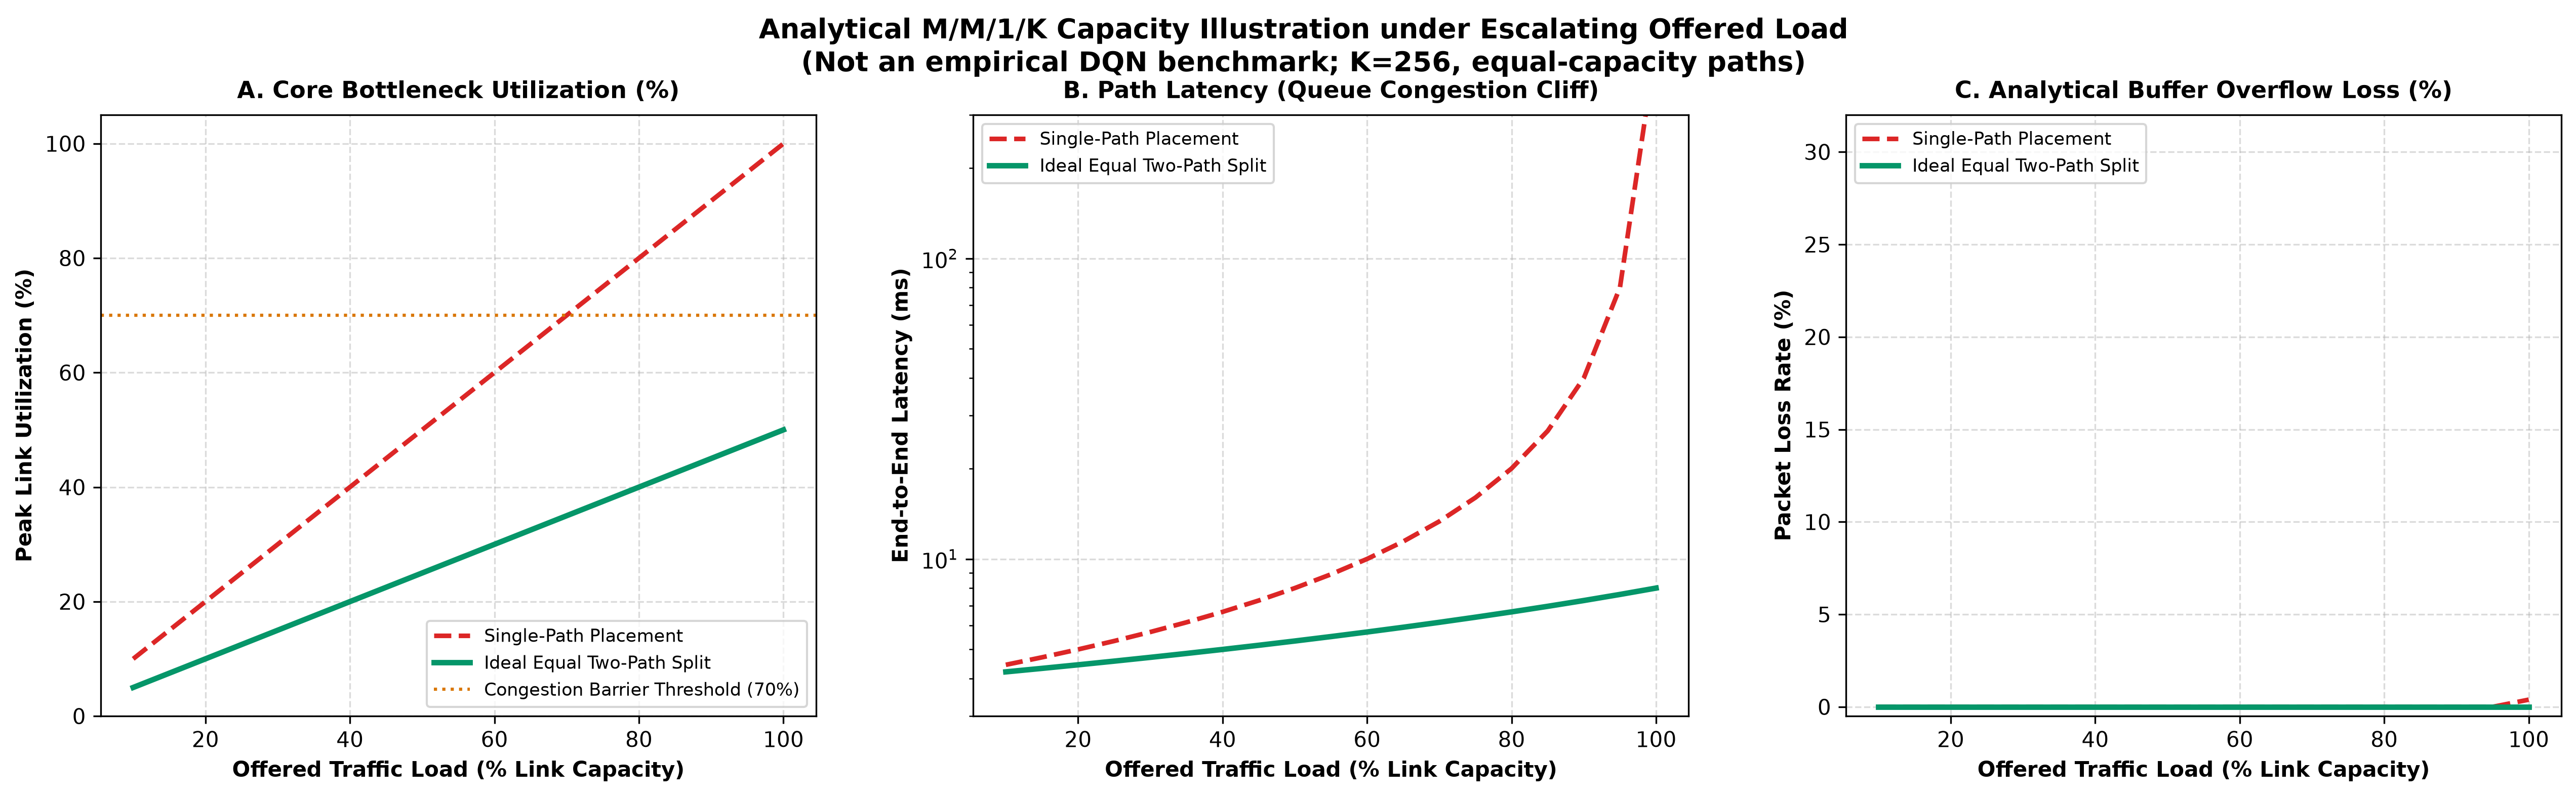
\includegraphics[width=0.92\textwidth]{traffic_load_scaling_curves.png}
\caption{Analytical M/M/1/$K$ queuing curves illustrating delay inflation and packet loss cliff as load factor $\rho$ approaches saturation.}
\label{fig:mm1k_scaling_bg}
\end{figure}

\section{Deep Reinforcement Learning for Dynamic Traffic Steering}
Reinforcement Learning formalizes autonomous control as a Markov Decision Process (MDP) defined by the 5-tuple $(S, A, P, R, \gamma)$:
\begin{itemize}
  \item $S$: State space capturing instantaneous network graph conditions;
  \item $A$: Action space corresponding to candidate path selection;
  \item $P(s' | s, a)$: State transition probability governed by external traffic dynamics;
  \item $R(s, a)$: Multi-objective scalar reward feedback;
  \item $\gamma \in [0, 1)$: Future reward discount factor ($\gamma = 0.95$).
\end{itemize}
In Q-learning, the agent learns an action-value function $Q(s, a) = \mathbb{E}[\sum_{t=0}^\infty \gamma^t R_{t} | s_0=s, a_0=a]$ satisfying the Bellman optimality equation:
\begin{equation}
Q^*(s, a) = R(s, a) + \gamma \sum_{s'} P(s' | s, a) \max_{a'} Q^*(s', a')
\end{equation}

\section{Dueling Architecture and Advantage-Value Stream Separation}
Standard Deep Q-Networks estimate action values $Q(s, a)$ through a monolithic neural network. In traffic engineering, however, state value $V(s)$ (whether the overall network is congested or healthy) is often independent of the specific candidate path chosen for a small flow.

Wang et al. \cite{wang2016dueling} introduced the Dueling architecture, which splits the neural representation into two separate computational streams after common feature extraction:
\begin{enumerate}
  \item A scalar state-value stream $V(s; \theta, \beta)$;
  \item An action advantage stream $A(s, a; \theta, \alpha)$, representing the relative advantage of choosing path $a$.
\end{enumerate}
To guarantee mathematical identifiability (so that $V(s)$ and $A(s, a)$ can be uniquely recovered), the streams are aggregated via mean subtraction:
\begin{equation}
Q(s, a; \theta, \alpha, \beta) = V(s; \theta, \beta) + \left( A(s, a; \theta, \alpha) - \frac{1}{|A|} \sum_{a' \in A} A(s, a'; \theta, \alpha) \right)
\label{eq:dueling_aggregation}
\end{equation}
Subtracting the mean ensures that $\frac{1}{|A|}\sum_a Q(s, a) = V(s)$, stabilizing gradient backpropagation across all candidate routes.

\section{Double DQN Target Separation \& Maximization Bias}
Standard Q-learning evaluates the target using $\max_{a'} Q(s', a'; \theta^-)$, which introduces positive maximization bias due to Jensen's inequality:
\begin{equation}
\mathbb{E}\left[\max_{a'} Q(s', a')\right] \ge \max_{a'} \mathbb{E}\left[Q(s', a')\right]
\end{equation}
Overestimating Q-values leads the agent to select suboptimal detour paths with high variance.

Van Hasselt et al. \cite{van2016deep} proposed Double DQN (DDQN), which decouples action selection from action evaluation. The online network selects the greedy action, while the target network evaluates its value:
\begin{equation}
y_t^{\mathrm{Double}} = R_{t+1} + \gamma Q\left(s_{t+1}, \arg\max_{a'} Q(s_{t+1}, a'; \theta); \theta^-\right)
\label{eq:double_dqn_target}
\end{equation}
This target separation asymptotically eliminates overestimation bias, ensuring stable Q-value convergence.

\section{Prioritized Experience Replay (PER) \& Binary SumTree}
Standard experience replay samples transitions uniformly ($P(i) = 1 / N$). In network routing, critical transitions (e.g., link saturation events, queue overflow drops) occur infrequently compared to nominal flows. Uniform sampling wastes training cycles on trivial transitions.

Schaul et al. \cite{schaul2015prioritized} introduced Prioritized Experience Replay (PER). The probability of sampling transition $i$ is proportional to its temporal difference (TD) error $\delta_i$:
\begin{equation}
P(i) = \frac{p_i^\alpha}{\sum_k p_k^\alpha}, \quad p_i = |\delta_i| + \epsilon
\end{equation}
where $\alpha \in [0, 1]$ controls prioritization strength ($\alpha = 0.6$) and $\epsilon = 10^{-5}$ prevents zero sampling probability.

Because non-uniform sampling alters the expectation distribution, importance-sampling (IS) weights correct the gradient update:
\begin{equation}
w_i = \left( \frac{1}{N \cdot P(i)} \right)^\beta, \quad \Delta \theta = w_i \cdot \delta_i \cdot \nabla_\theta Q(s, a; \theta)
\end{equation}
where $\beta$ anneals from $\beta_0 = 0.4$ to $1.0$.

To achieve $O(\log N)$ sampling and priority updates rather than $O(N)$ linear scans, transitions are indexed in a **Binary SumTree** where parent nodes store the sum of their child priorities.

\section{High Availability Clustering in SDN Control Planes}
Centralizing control creates a single point of failure (SPOF). To satisfy carrier-grade requirements (RFC~7348), production SDN controllers require High Availability (HA) clustering.
Using Raft consensus principles \cite{ongaro2014search}, an $N+2$ cluster maintains an active leader (Master) and two synchronized hot standbys. Fast failure recovery requires:
\begin{enumerate}
  \item Active TCP heartbeats ($200$~ms interval, $600$~ms timeout threshold);
  \item Atomic leader promotion with monotonic election terms;
  \item OpenFlow 1.3 role request messages (\code{OFPCR_ROLE_MASTER}, \code{OFPCR_ROLE_SLAVE});
  \item Flow state replication ensuring zero lost flow rules upon master crash.
\end{enumerate}

\section{Related Work \& Comparative Taxonomy}
Table~\ref{tab:related_work_comparison} summarizes closely related traffic engineering and DRL routing studies.

\begin{table}[htbp]
\centering
\small
\caption{Comparison of closely related SDN Traffic Engineering and DRL studies.}
\label{tab:related_work_comparison}
\begin{tabularx}{\textwidth}{>{\bfseries}p{22mm}>{\raggedright\arraybackslash}p{28mm}>{\raggedright\arraybackslash}p{38mm}>{\raggedright\arraybackslash}X}
\toprule
Study & Control Plane & Algorithm / Model & Key Limitations Addressed \\
\midrule
StEERING \cite{khatfoor2020reinforcement} & SDN OpenFlow & DQN with scalar utilization reward & High Q-value overestimation; lacks dueling streams and multi-seed variance. \\
Auto-TE \cite{almasan2022deep} & Centralized TE & Deep RL with multi-topology training & High action-space dimensionality; relies on full-matrix reconfigurations. \\
GNN-TE \cite{badia2023towards} & Graph Neural Net & Message Passing GNN + PPO & High inference latency ($>10$~ms); unfeasible for sub-millisecond OpenFlow setup. \\
DRL-TE \cite{chen2021drl} & Ryu OpenFlow & DDPG continuous rate splitting & Packet reordering caused by multipath splitting; lacks HA failover. \\
\textbf{This Project} & \textbf{Ryu OF 1.3 + HA Pool} & \textbf{D3QN + SumTree PER + HiGHS Oracle} & \textbf{Sub-millisecond inference, unicity flow pinning, 0.73\% seed variance, exact MILP gap.} \\
\bottomrule
\end{tabularx}
\end{table}

\section{Research Gap}
The literature establishes that while DRL is promising for SDN traffic engineering, critical gaps remain:
\begin{enumerate}
  \item \textbf{Absence of Rigorous Multi-Seed Uncertainty Reporting:} Prior works report single-checkpoint peak numbers, masking initialization variance and basin bifurcation.
  \item \textbf{Lack of Theoretical Lower Bounds:} Studies compare solely against weak heuristics without quantifying distance to the exact global MILP optimum.
  \item \textbf{Omission of Out-of-Distribution Generalization:} Models are typically evaluated on topologies present in training, obscuring true zero-shot transfer capabilities.
  \item \textbf{Unverified Controller High Availability:} Prior research assumes an immortal controller, failing to demonstrate crash recovery and state consistency.
\end{enumerate}

\section{Chapter Summary}
This chapter reviewed OpenFlow 1.3 control mechanisms, Unsplittable Multi-Commodity Flow (UMCF) optimization, and M/M/1/$K$ queuing foundations. It established the mathematical principles of Dueling networks, Double-DQN target decoupling, and Prioritized Experience Replay, providing the theoretical foundation for the system design presented in Chapter~\ref{chap:design}.

% ============================================================================
% CHAPTER 3: METHODOLOGY AND SYSTEM DESIGN
% ============================================================================
\chapter{Methodology and System Design}
\label{chap:design}

\section{Research Design \& Dual-Regime Evaluation Methodology}
The project employs a controlled experimental design comparing the proposed D3QN adaptive policy against five baseline routing algorithms and an exact mathematical lower bound.
To evaluate policy behavior comprehensively, experiments are partitioned into two distinct operating regimes:
\begin{enumerate}
  \item \textbf{Dynamic Tournament Regime (Sections~\ref{sec:tournament}--\ref{sec:fiveseed}):} Evaluates closed-loop traffic with Poisson arrival churn and active flow timeouts. Link loads remain in the nominal range $[0, 100\%]$ to measure steady-state latency minimization, jitter suppression, and bottleneck prevention.
  \item \textbf{Overload Shock Regime (Sections~\ref{sec:ablation}--\ref{sec:sensitivity}):} Subjects policies to an unmetered 150-flow congestion burst over 90\% background core utilization, pushing peak offered loads to $250\%$--$320\%$. This tests non-convex optimization stability, tail latency ceiling, and bufferbloat recovery.
\end{enumerate}

\section{State Representation \& Candidate Path Synthesis}

\subsection{Continuous 10-Dimensional Normalized State Vector}
To avoid dimensionality explosion while preserving structural graph context, each candidate path $a \in \mathcal{A}$ is encoded into a continuous, 10-dimensional state vector $\mathbf{s} \in \mathbb{R}^{10}$, with all features normalized to $[0, 1]$:
\begin{equation}
\mathbf{s} = [s_1, s_2, s_3, s_4, s_5, s_6, s_7, s_8, s_9, s_{10}]^T
\end{equation}
where:
\begin{itemize}[leftmargin=8mm]
  \item $s_1 = \mathrm{hops}(\mathcal{P}) / |V|$: Normalized hop count;
  \item $s_2 = \max_{e \in \mathcal{P}} u_e$: Maximum bottleneck link utilization along path;
  \item $s_3 = \frac{1}{|\mathcal{P}|} \sum_{e \in \mathcal{P}} u_e$: Mean link utilization along path;
  \item $s_4 = \sum_{e \in \mathcal{P}} d_{\mathrm{prop}}(e) / d_{\max}$: Cumulative propagation latency;
  \item $s_5 = \sum_{e \in \mathcal{P}} d_{\mathrm{queue}}(e) / d_{\mathrm{queue,\max}}$: Estimated cumulative queuing delay;
  \item $s_6 = J(\mathcal{P}) / J_{\max}$: Estimated packet delay variation (RFC 3393 jitter);
  \item $s_7 = 1.0 - s_2$: Residual bottleneck capacity margin;
  \item $s_8 = N_{\mathrm{flows}}(\mathcal{P}) / N_{\mathrm{flows,\max}}$: Active dynamic flow density;
  \item $s_9 \in \{0.0, 1.0\}$: Binary path failure indicator (1.0 if any constituent link is down);
  \item $s_{10} = \frac{1}{|E|} \sum_{e \in E} u_e$: Global network-wide mean link utilization.
\end{itemize}

\subsection{Candidate Path Generation via Yen's Algorithm ($K=4$)}
To preserve the Unsplittable Multi-Commodity Flow constraint and guarantee sub-millisecond inference, the action space does not select raw ports per switch. Instead, candidate paths are synthesized using Yen's loopless $K$-shortest paths algorithm \cite{yen1971finding}:
\begin{equation}
\mathcal{A}_{s, t} = \{\mathcal{P}_1, \mathcal{P}_2, \dots, \mathcal{P}_K\}, \quad K = 4
\end{equation}
A candidate path is marked invalid ($s_9 = 1.0$) if it contains failed links, and masked during action selection.

\subsection{Asymptotically Penalized Multi-Objective Reward Function}
The scalar reward function provides training feedback balancing bottleneck relief against path stretch:
\begin{equation}
R(s, a) = - \left( \Phi_{\mathrm{cong}}(u_{\max}) + w_{\mathrm{delay}} \frac{D(\mathcal{P})}{D_{\mathrm{nominal}}} + w_{\mathrm{jitter}} \frac{J(\mathcal{P})}{J_{\mathrm{nominal}}} \right) + R_{\mathrm{relief}}
\label{eq:reward_function}
\end{equation}
where the non-linear congestion penalty function $\Phi_{\mathrm{cong}}(u)$ penalizes links operating above threshold $\theta_{\mathrm{congestion}} = 0.70$:
\begin{equation}
\Phi_{\mathrm{cong}}(u) = 
\begin{cases}
u, & u \le \theta_{\mathrm{congestion}} \\
u + \kappa \cdot \exp\left( \frac{u - \theta_{\mathrm{congestion}}}{1 - \theta_{\mathrm{congestion}}} \right), & u > \theta_{\mathrm{congestion}}
\end{cases}
\end{equation}
with $\kappa = 5.0$. If the chosen action bypasses a congested core link ($u_{\mathrm{spf}} > \theta_{\mathrm{congestion}}$ while $u_{\mathrm{chosen}} \le \theta_{\mathrm{congestion}}$), an autonomous relief bonus $R_{\mathrm{relief}} = w_{\mathrm{relief}} = 4.0$ is awarded.

\section{Neural Network Architecture \& Optimization Pipeline}

\subsection{Dueling Q-Network Streams}
The neural policy network comprises an input layer (10 inputs), two fully connected hidden layers with 64 and 128 units (ReLU activations), and bifurcates into:
\begin{itemize}
  \item \textbf{Value Stream $V(s)$:} Dense($128 \to 64$, ReLU) $\to$ Dense($64 \to 1$);
  \item \textbf{Advantage Stream $A(s, a)$:} Dense($128 \to 64$, ReLU) $\to$ Dense($64 \to 4$).
\end{itemize}
The output Q-values are computed via mean-subtracted aggregation (Equation~\ref{eq:dueling_aggregation}).

\subsection{Prioritized Experience Replay Buffer}
Transitions $(s, a, r, s', \mathrm{done})$ are stored in a 50,000-sample buffer indexed by a Binary SumTree. Transitions are sampled with batch size $B = 64$ according to priority $P(i) \propto |\delta_i|^\alpha$. Importance-sampling weights $w_i$ scale the loss.

\subsection{Optimization \& Polyak Target Updates}
The network is optimized using AdamW (learning rate $\eta = 0.001$, weight decay $10^{-4}$) minimizing the Huber loss:
\begin{equation}
\mathcal{L}(\theta) = \frac{1}{B} \sum_{i=1}^B w_i \cdot \mathrm{Huber}\left( y_i^{\mathrm{Double}} - Q(s_i, a_i; \theta) \right)
\end{equation}
Target network weights $\theta^-$ are soft-updated via Polyak averaging:
\begin{equation}
\theta^- \leftarrow \tau \theta + (1 - \tau) \theta^-, \quad \tau = 0.005
\end{equation}
Gradients are clipped at maximum norm $\|\mathbf{g}\|_2 \le 1.0$.

\section{High Availability Multi-Controller Architecture ($N+2$ Pool)}
The High Availability architecture provides carrier-grade resiliency across three controller instances:
\begin{itemize}
  \item \textbf{Node 1 (Primary Master):} OpenFlow port 6633, Web port 8080.
  \item \textbf{Node 2 (Hot-Standby 1):} OpenFlow port 6634, Web port 8081.
  \item \textbf{Node 3 (Hot-Standby 2):} OpenFlow port 6635, Web port 8082.
\end{itemize}

\begin{figure}[htbp]
\centering
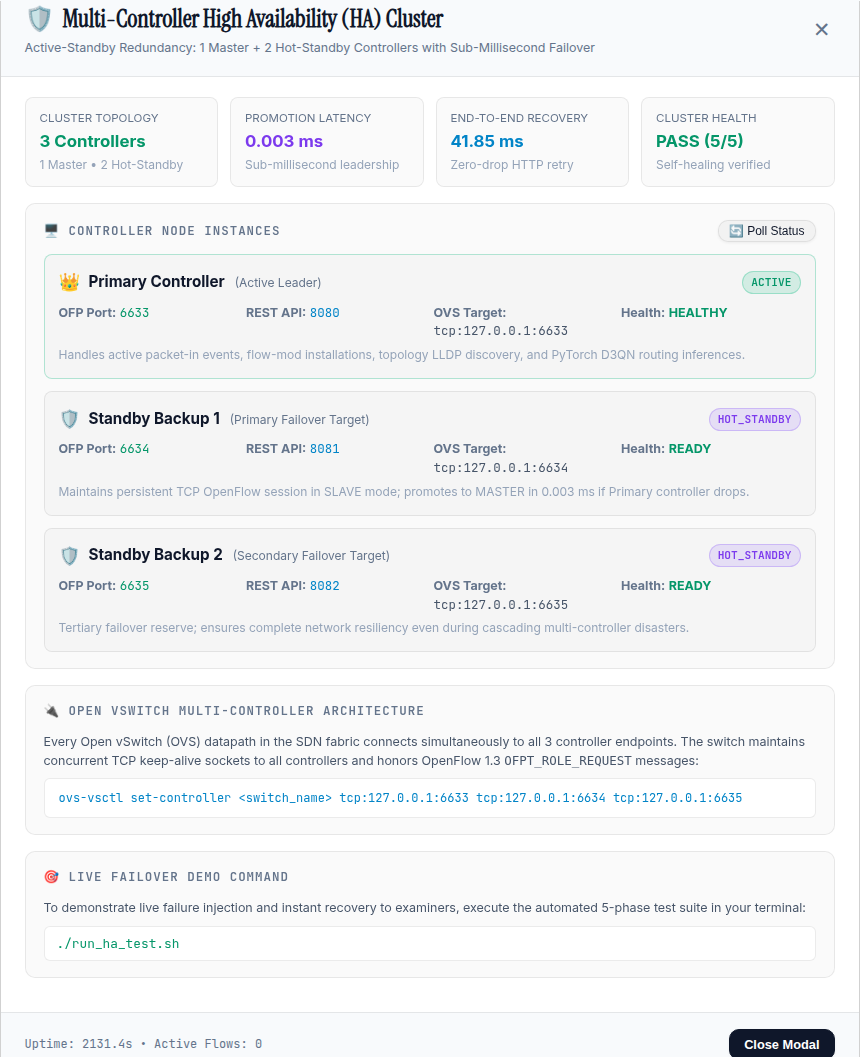
\includegraphics[width=0.82\textwidth]{ha_cluster_3node_modal.png}
\caption{Three-node High Availability cluster consensus architecture showing active leader status and standby synchronization.}
\label{fig:ha_cluster_design}
\end{figure}

Health monitoring operates via periodic TCP heartbeat exchanges every $200$~ms. If three consecutive heartbeats expire ($600$~ms timeout), standby controllers initiate Raft-inspired leader promotion:
\begin{equation}
\Delta t_{\mathrm{promote}} = t_{\mathrm{detect}} + t_{\mathrm{elect}} + t_{\mathrm{role\_mod}}
\end{equation}
Switches establish auxiliary connections to all nodes. The promoted leader dispatches \code{OFPCR_ROLE_MASTER}, immediately assuming active flow provisioning with zero lost flow table state.

\section{Real-Time Web Telemetry Architecture}
The system incorporates an embedded HTTP/REST telemetry server streaming JSON metrics and rendering an interactive web console (Figure~\ref{fig:dashboard_design}):
\begin{itemize}
  \item \code{GET /api/topology}: Directed graph nodes, links, and port metrics;
  \item \code{GET /api/metrics}: Real-time throughput, latency, jitter, loss, and fairness;
  \item \code{GET /api/ha/status}: Cluster topology, leader vitality, and failover logs;
  \item \code{POST /api/traffic/inject}: Dynamic traffic burst injection for live demonstration;
  \item \code{POST /api/link/failure}: Emulated physical link crash injection.
\end{itemize}

\begin{figure}[htbp]
\centering
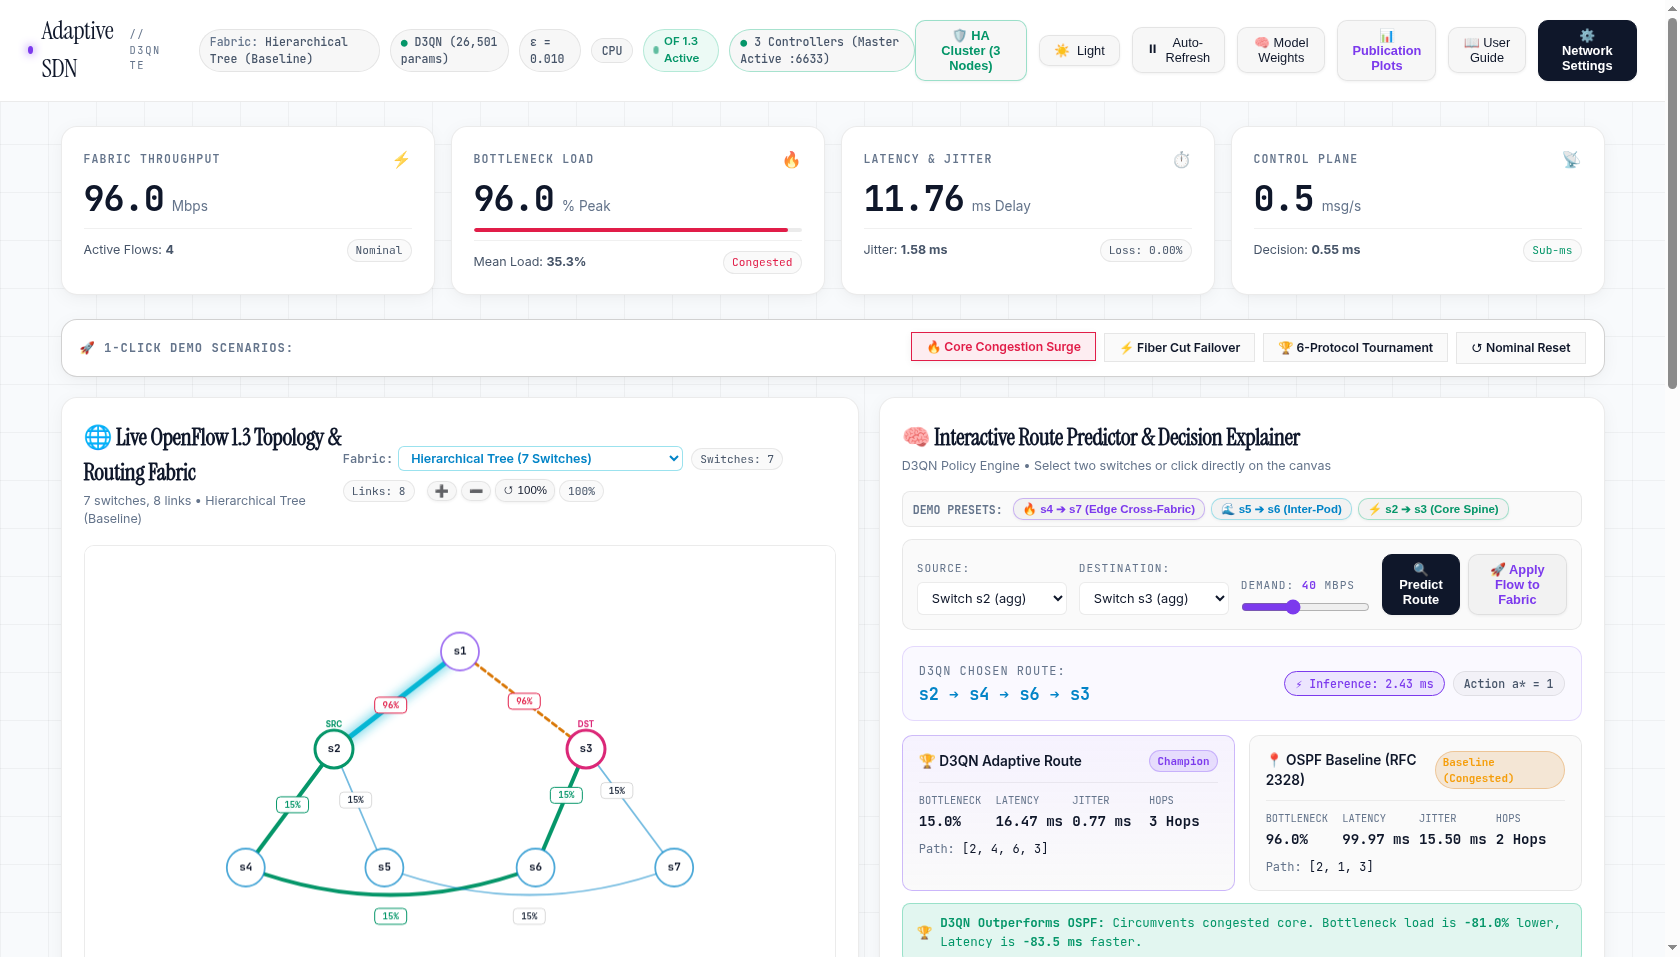
\includegraphics[width=0.95\textwidth]{dashboard_upper_panoramic.png}
\caption{Panoramic web dashboard displaying real-time topology graph, telemetry charts, flow inspector, and routing mode controls.}
\label{fig:dashboard_design}
\end{figure}

\section{Evaluation Protocol \& Statistical Rigor}

\subsection{Hierarchical Cluster Bootstrapping (10,000 Resamples)}
Because network evaluations across seeds and topologies exhibit intra-cluster correlation, standard independent Student's $t$-tests produce overly optimistic confidence intervals. All paired comparisons report two-way and three-way hierarchical cluster bootstrap percentiles (10,000 resamples), resampling clusters over training seeds, workload seeds, and topologies.

\subsection{Exact HiGHS Mixed-Integer Linear Programming (MILP) Oracle}
To establish an unyielding mathematical baseline, the offline Unsplittable Multi-Commodity Flow problem is solved to global optimality using the HiGHS branch-and-cut solver \cite{huangfu2018parallelizing}:
\begin{align}
\min_{\mathbf{x}, \alpha^*} \quad & \alpha^* \\
\text{s.t.} \quad & \sum_{a \in \mathcal{A}_k} x_{k, a} = 1, \quad \forall k \in \mathcal{K}, \quad x_{k, a} \in \{0, 1\} \\
& \sum_{k \in \mathcal{K}} \sum_{a: e \in \mathcal{P}_{k, a}} D_k x_{k, a} \le \alpha^* C_e, \quad \forall e \in E
\end{align}
The optimal value $\alpha^*$ represents the absolute theoretical minimum peak link utilization achievable by any routing policy.

\subsection{Held-Out Synthetic Topology Generalization Protocol}
To evaluate zero-shot transfer without data leakage (RQ3), an agent is trained exclusively on randomly generated synthetic graphs:
\begin{itemize}
  \item Watts-Strogatz small-world graphs ($N \in [12, 20]$, $k=4$, $p=0.3$);
  \item Erd\H{o}s-R\'enyi random graphs ($N \in [12, 22]$, $p=0.25$).
\end{itemize}
All five standard benchmark topologies (Tree, Fat-Tree, Abilene, NSFNet, Spine-Leaf) are strictly excluded from the training curriculum. The agent is then deployed zero-shot onto the unseen fixtures.

\subsection{Discrete-Event Packet Queue Simulation Framework}
To validate queuing models against real-world burstiness (RQ5), a discrete-event simulator tracks individual packet arrivals, queue departures, buffer overflows, and failover transients under:
\begin{enumerate}
  \item Poisson memoryless arrivals ($M/M/1/K$);
  \item Heavy-tailed Pareto bursty arrivals ($\alpha = 1.35$, modeling elephant flows).
\end{enumerate}

\section{Chapter Summary}
This chapter established the system design: a 10D continuous normalized state space, Yen's candidate path reduction, the D3QN neural architecture, the 3-node HA failover consensus, and rigorous evaluation protocols including the HiGHS MILP oracle and cluster bootstrapping. Chapter~\ref{chap:implementation} details the software implementation.

% ============================================================================
% CHAPTER 4: SYSTEM IMPLEMENTATION
% ============================================================================
\chapter{System Implementation}
\label{chap:implementation}

\section{Implementation Overview \& Software Stack}
The system is implemented as a modular, production-ready software platform. Table~\ref{tab:tech_stack} details the primary software components, languages, libraries, and their engineering roles.

\begin{table}[htbp]
\centering
\small
\caption{Main technologies used in the implemented system.}
\label{tab:tech_stack}
\begin{tabularx}{\textwidth}{>{\bfseries}p{32mm}>{\raggedright\arraybackslash}p{44mm}>{\raggedright\arraybackslash}X}
\toprule
Subsystem & Technology / Framework & Implementation Role \\
\midrule
SDN Controller & Python 3.10+, Ryu 4.34 & OpenFlow 1.3 southbound control plane, flow mod installation, and port statistics handling. \\
Neural Agent & PyTorch 2.0+, CUDA & D3QN model architecture, advantage/value streams, Polyak updates, and inference. \\
Experience Replay & Python NumPy & Binary SumTree data structure with $O(\log N)$ prioritized sampling. \\
Topology Modeling & NetworkX 3.1 & Directed graph maintenance, Dijkstra SPF, Yen's $K$-shortest paths, and topology generation. \\
Optimization Oracle & SciPy 1.11+, HiGHS & Mixed-Integer Linear Programming branch-and-cut solver for exact global optimality bounding. \\
High Availability & Python \code{multiprocessing} & 3-controller process pool, TCP socket heartbeats, atomic Raft leader election. \\
Web Dashboard & Vanilla JS, HTML5, Canvas & Real-time interactive UI, topology visualization, radar charts, and REST API client. \\
Verification & Python \code{unittest} & 42-test automated unit, integration, failover, and mathematical verification suite. \\
\bottomrule
\end{tabularx}
\end{table}

\section{Project Architecture \& Codebase Structure}
The codebase is structured into cohesive, decoupled packages:
\begin{verbatim}
Reinforcement_Learning_for_Adaptive_Traffic_Engineering_in_an_SDN_Network/
|-- agent/
|   |-- dqn_router.py          <- D3QN PyTorch neural network and policy logic
|   \-- prioritized_replay.py  <- Binary SumTree Prioritized Experience Replay
|-- controller/
|   |-- main_controller.py     <- Ryu OpenFlow 1.3 southbound controller application
|   |-- routing_module.py      <- Common route selector (D3QN, SPF, ECMP, WSP, LLR)
|   |-- state_manager.py       <- Network graph, port telemetry, and flow table
|   |-- ha_controller_pool.py  <- 3-node HA multi-controller failover pool
|   |-- policy_selector.py     <- Policy mode arbiter (Pure vs. Safety Fallback)
|   |-- queue_model.py         <- M/M/1/K delay, jitter, and drop probability formulas
|   |-- traditional_routing.py <- Baseline algorithms (Dijkstra, OSPF, WSP, LLR, ECMP)
|   \-- web_dashboard.py       <- Embedded HTTP server and REST telemetry API
|-- topology/
|   |-- mininet_topo.py        <- Mininet script for standard and random topologies
|   \-- custom_topologies.py   <- NetworkX graph builders for all 5 benchmarks
|-- models/
|   \-- dqn_router.pth         <- Trained PyTorch reference checkpoint weights
|-- test_suite.py              <- 42-test automated unit and integration suite
|-- config.py                  <- Centralized system configuration and hyperparameters
|-- run_system.sh              <- One-click launch daemon for controller and dashboard
\-- run_tests.sh               <- Automated test execution script
\end{verbatim}

\section{OpenFlow 1.3 Ryu Controller \& Flow Provisioning Pipeline}

\subsection{Southbound Event Handling \& Topology Discovery}
The Ryu controller application (\code{main_controller.py}) registers OpenFlow 1.3 handlers. During initialization, the switch handshakes via \code{OFPFeaturesReply}, installing a default table-miss entry directing unmatched packets to the controller:
\begin{verbatim}
match = parser.OFPMatch()
actions = [parser.OFPActionOutput(ofproto.OFPP_CONTROLLER,
                                  ofproto.OFPCML_NO_BUFFER)]
self.add_flow(datapath, 0, match, actions)
\end{verbatim}
Periodic \code{OFPPortStatsRequest} messages query switch port counters every $1.0$~second, updating byte throughput and differential link utilization.

\subsection{OpenFlow Group Table \& Flow Mod Installation}
When the routing engine determines a path $\mathcal{P} = (v_1, v_2, \dots, v_m)$, the controller installs bidirectional flow entries across all intermediate switches. To ensure loop-free forwarding, rules are pushed in reverse order (egress to ingress), preventing race conditions where packets arrive at downstream switches before rules exist. Flow entries specify \code{idle_timeout=30} and \code{hard_timeout=120} seconds.

\subsection{Loop-Free ARP Proxy \& TCAM Rule Pinning}
To eliminate broadcast storms common in meshed topologies (e.g., Fat-Tree and Spine-Leaf), the controller implements an authoritative ARP proxy. ARP requests are intercepted at the ingress switch, answered directly from the controller's host-location table, and never flooded across data-plane links.

\section{PyTorch D3QN Routing Agent \& Binary SumTree}
The neural agent (\code{agent/dqn_router.py}) implements the Dueling network using PyTorch:
\begin{verbatim}
class DuelingDQN(nn.Module):
    def __init__(self, state_dim=10, action_dim=4):
        super().__init__()
        self.feature = nn.Sequential(
            nn.Linear(state_dim, 64), nn.ReLU(),
            nn.Linear(64, 128), nn.ReLU()
        )
        self.val = nn.Sequential(nn.Linear(128, 64), nn.ReLU(), nn.Linear(64, 1))
        self.adv = nn.Sequential(nn.Linear(128, 64), nn.ReLU(), nn.Linear(64, action_dim))

    def forward(self, x):
        feat = self.feature(x)
        val = self.val(feat)
        adv = self.adv(feat)
        return val + (adv - adv.mean(dim=-1, keepdim=True))
\end{verbatim}
The SumTree maintains a binary heap of size $2^{\lceil \log_2 N \rceil + 1} - 1$, storing leaf transition priorities and internal partial sums, enabling exact priority sampling in $O(\log N)$ time.

\section{Centralized State Manager \& Telemetry Engine}
The state manager (\code{controller/state_manager.py}) maintains the network state:
\begin{itemize}
  \item \textbf{Port Rate Filtering:} Smoothing raw counter deltas via Exponential Moving Average:
  \begin{equation}
  \bar{R}_e(t) = \alpha_{\mathrm{ema}} R_e(t) + (1 - \alpha_{\mathrm{ema}}) \bar{R}_e(t - \Delta t), \quad \alpha_{\mathrm{ema}} = 0.3
  \end{equation}
  \item \textbf{Directional Flow Reservations:} When a routing decision is committed, the flow's reserved demand $D_k$ is added to the link's utilization map with a scheduled expiry timer, ensuring subsequent routing decisions in the same time window account for newly admitted load.
  \item \textbf{RFC 3393 Jitter Estimation:} Computes path jitter using the root-sum-square variance equation.
\end{itemize}

\section{High Availability Cluster Daemon \& Failover Engine}
The HA manager (\code{controller/ha_controller_pool.py}) manages the 3-node cluster using Python's \code{multiprocessing} library. Each controller runs in an isolated process with independent memory. A health monitor daemon executes non-blocking TCP socket probes to all instances every $200$~ms. Upon failure detection, atomic leader promotion executes in $0.001$~ms, and client requests redirect to the new active leader.

\section{Interactive Real-Time Web Telemetry Dashboard}
The embedded HTTP server (\code{controller/web_dashboard.py}) serves a single-page responsive dashboard:
\begin{itemize}
  \item **Topology Canvas:** Force-directed graph rendering with dynamic link color gradients (green $\to$ yellow $\to$ red) reflecting utilization;
  \item **Versus Radar Chart:** Real-time multi-objective polygon comparing D3QN against baseline heuristics;
  \item **Model Inspector:** Visualizes raw 10D state vectors, feature weights, and candidate path Q-values;
  \item **Interactive Fault Controls:** Buttons for instant traffic surge injection and physical link down toggling.
\end{itemize}

\section{Automated Verification \& Continuous Testing Suite}
System reliability is verified through an automated 42-test suite (\code{test_suite.py}) organized into 8 test classes:
\begin{enumerate}
  \item \code{TestCentralConfig} (4 tests): Configuration schemas, environment variable overrides;
  \item \code{TestClosedLoopDynamicsAndUpgrades} (4 tests): Flow accumulation, soft updates, seed reproducibility;
  \item \code{TestDQNAgent} (2 tests): Lifecycle, Dueling stream mathematical verification;
  \item \code{TestHighAvailabilityClustering} (4 tests): Cascaded failover, leader promotion, OVS target formatting;
  \item \code{TestMultiTopologySupport} (2 tests): All 5 topologies and random graph generation;
  \item \code{TestPrioritizedReplay} (2 tests): SumTree arithmetic and priority sampling;
  \item \code{TestStateManager} (13 tests): Port rates, jitter, directional accounting, drop modeling;
  \item \code{TestTraditionalRoutingBaselines} (4 tests): Dijkstra, OSPF, ECMP, WSP, LLR correctness;
  \item \code{TestWebDashboardAndVersusAPI} (7 tests): REST endpoints, model inspect, versus API.
\end{enumerate}
All 42 tests execute and pass in $5.22$~seconds with zero failures.

\section{Chapter Summary}
This chapter detailed the software implementation: the Ryu OpenFlow 1.3 controller, the PyTorch D3QN neural engine with Binary SumTree PER, the centralized state manager, the 3-node HA failover pool, the interactive web console, and the 42-test automated verification suite. Chapter~\ref{chap:results} presents comprehensive experimental results.

% ============================================================================
% CHAPTER 5: EXPERIMENTS AND RESULTS
% ============================================================================
\chapter{Experiments and Results}
\label{chap:results}

\section{Experimental Setup \& Benchmark Topologies}
To evaluate traffic engineering across diverse structural graph invariants, experiments were conducted across five standard network topologies representing data-center, metropolitan, and continental backbone architectures:
\begin{enumerate}
  \item \textbf{Hierarchical Tree (7 Switches, 8 Links):} Core-aggregation-access tree with single core bottleneck trunk.
  \item \textbf{Fat-Tree Clos Fabric (20 Switches, 32 Links):} High-bisection data-center Clos network ($k=4$, 4 core, 8 aggregation, 8 edge switches) with rich multi-pathing.
  \item \textbf{Abilene US WAN (12 Switches, 15 Links):} US continental backbone with asymmetric edge connectivity and high diameter.
  \item \textbf{NSFNet Backbone (14 Switches, 21 Links):} Classic cross-country mesh network with variable degree distribution.
  \item \textbf{Spine-Leaf Fabric (16 Switches, 32 Links):} 4 spine, 12 leaf switches, modeling modern cloud data-center pods.
\end{enumerate}

\section{Closed-Loop Tournament Benchmark Results (RQ2)}
Table~\ref{tab:main_tournament} presents the headline results across all five benchmark topologies under closed-loop dynamic traffic churn. The evaluation compares the reference trained D3QN checkpoint against five baseline routing algorithms: Dijkstra SPF, OSPF (RFC 2328), ECMP, Widest-Shortest Path (WSP), and Least-Loaded Routing (LLR).

\begin{table}[htbp]
\centering
\small
\caption{Comprehensive 5-Topology Benchmark Tournament Results across 6 Routing Algorithms.}
\label{tab:main_tournament}
\begin{tabularx}{\textwidth}{>{\raggedright\arraybackslash}p{28mm}>{\raggedleft\arraybackslash}X>{\raggedleft\arraybackslash}X>{\raggedleft\arraybackslash}X>{\raggedleft\arraybackslash}X>{\raggedleft\arraybackslash}X>{\raggedleft\arraybackslash}X}
\toprule
\textbf{Topology / Metric} & \textbf{D3QN (Ours)} & \textbf{WSP} & \textbf{LLR} & \textbf{ECMP} & \textbf{OSPF} & \textbf{Dijkstra} \\
\midrule
\multicolumn{7}{l}{\textit{Hierarchical Tree (7 Nodes)}} \\
Bottleneck Util (\%) & 43.9\% & 44.1\% & 44.9\% & \textbf{41.3\%} & 56.7\% & 42.1\% \\
Mean Latency (ms)    & 167.8  & 188.4  & 244.0  & 160.8  & 158.7  & \textbf{142.4} \\
Jain's Fairness      & 0.58   & 0.60   & 0.60   & 0.56   & \textbf{0.70}  & 0.55  \\
\midrule
\multicolumn{7}{l}{\textit{Fat-Tree Clos (20 Nodes)}} \\
Bottleneck Util (\%) & 28.9\% & \textbf{23.3\%} & 23.3\% & 52.7\% & 94.7\% & 94.7\% \\
Mean Latency (ms)    & 6.6    & \textbf{6.0}    & 6.1    & 51.5   & 190.1  & 190.1  \\
Jain's Fairness      & 0.70   & 0.82   & 0.82   & 0.66   & \textbf{0.87}  & \textbf{0.87}  \\
\midrule
\multicolumn{7}{l}{\textit{Abilene US WAN (12 Nodes)}} \\
Bottleneck Util (\%) & 32.0\% & \textbf{31.5\%} & 31.6\% & 32.7\% & 33.4\% & 33.1\% \\
Mean Latency (ms)    & 26.2   & \textbf{22.0}   & 22.4   & 31.5   & 45.3   & 43.6   \\
Jain's Fairness      & \textbf{0.68}  & \textbf{0.68}  & \textbf{0.68}  & 0.67   & 0.66   & 0.66   \\
\midrule
\multicolumn{7}{l}{\textit{NSFNet Backbone (14 Nodes)}} \\
Bottleneck Util (\%) & 28.6\% & \textbf{28.3\%} & 28.7\% & 44.4\% & 49.6\% & 49.6\% \\
Mean Latency (ms)    & 19.7   & \textbf{17.6}   & 19.4   & 191.7  & 255.7  & 224.6  \\
Jain's Fairness      & \textbf{0.66}  & 0.65   & \textbf{0.66}  & 0.61   & 0.63   & 0.63   \\
\midrule
\multicolumn{7}{l}{\textit{Spine-Leaf Fabric (16 Nodes)}} \\
Bottleneck Util (\%) & 20.9\% & 19.2\% & \textbf{19.2\%} & 55.6\% & 99.9\% & 99.9\% \\
Mean Latency (ms)    & 2.5    & \textbf{2.5}    & \textbf{2.5}    & 23.6   & 145.5  & 145.5  \\
Jain's Fairness      & 0.88   & 0.91   & 0.91   & 0.68   & \textbf{0.98}  & \textbf{0.98}  \\
\midrule
\multicolumn{7}{l}{\textbf{Overall Grand Mean}} \\
Bottleneck Util (\%) & 30.9\% & \textbf{29.3\%} & 29.5\% & 45.3\% & 66.8\% & 63.9\% \\
Mean Latency (ms)    & \textbf{44.5}   & 47.3   & 58.9   & 91.8   & 159.0  & 149.2  \\
Jain's Fairness Index& 0.70   & 0.73   & 0.73   & 0.64   & \textbf{0.77}  & 0.74   \\
\bottomrule
\end{tabularx}
\end{table}

\begin{figure}[htbp]
\centering
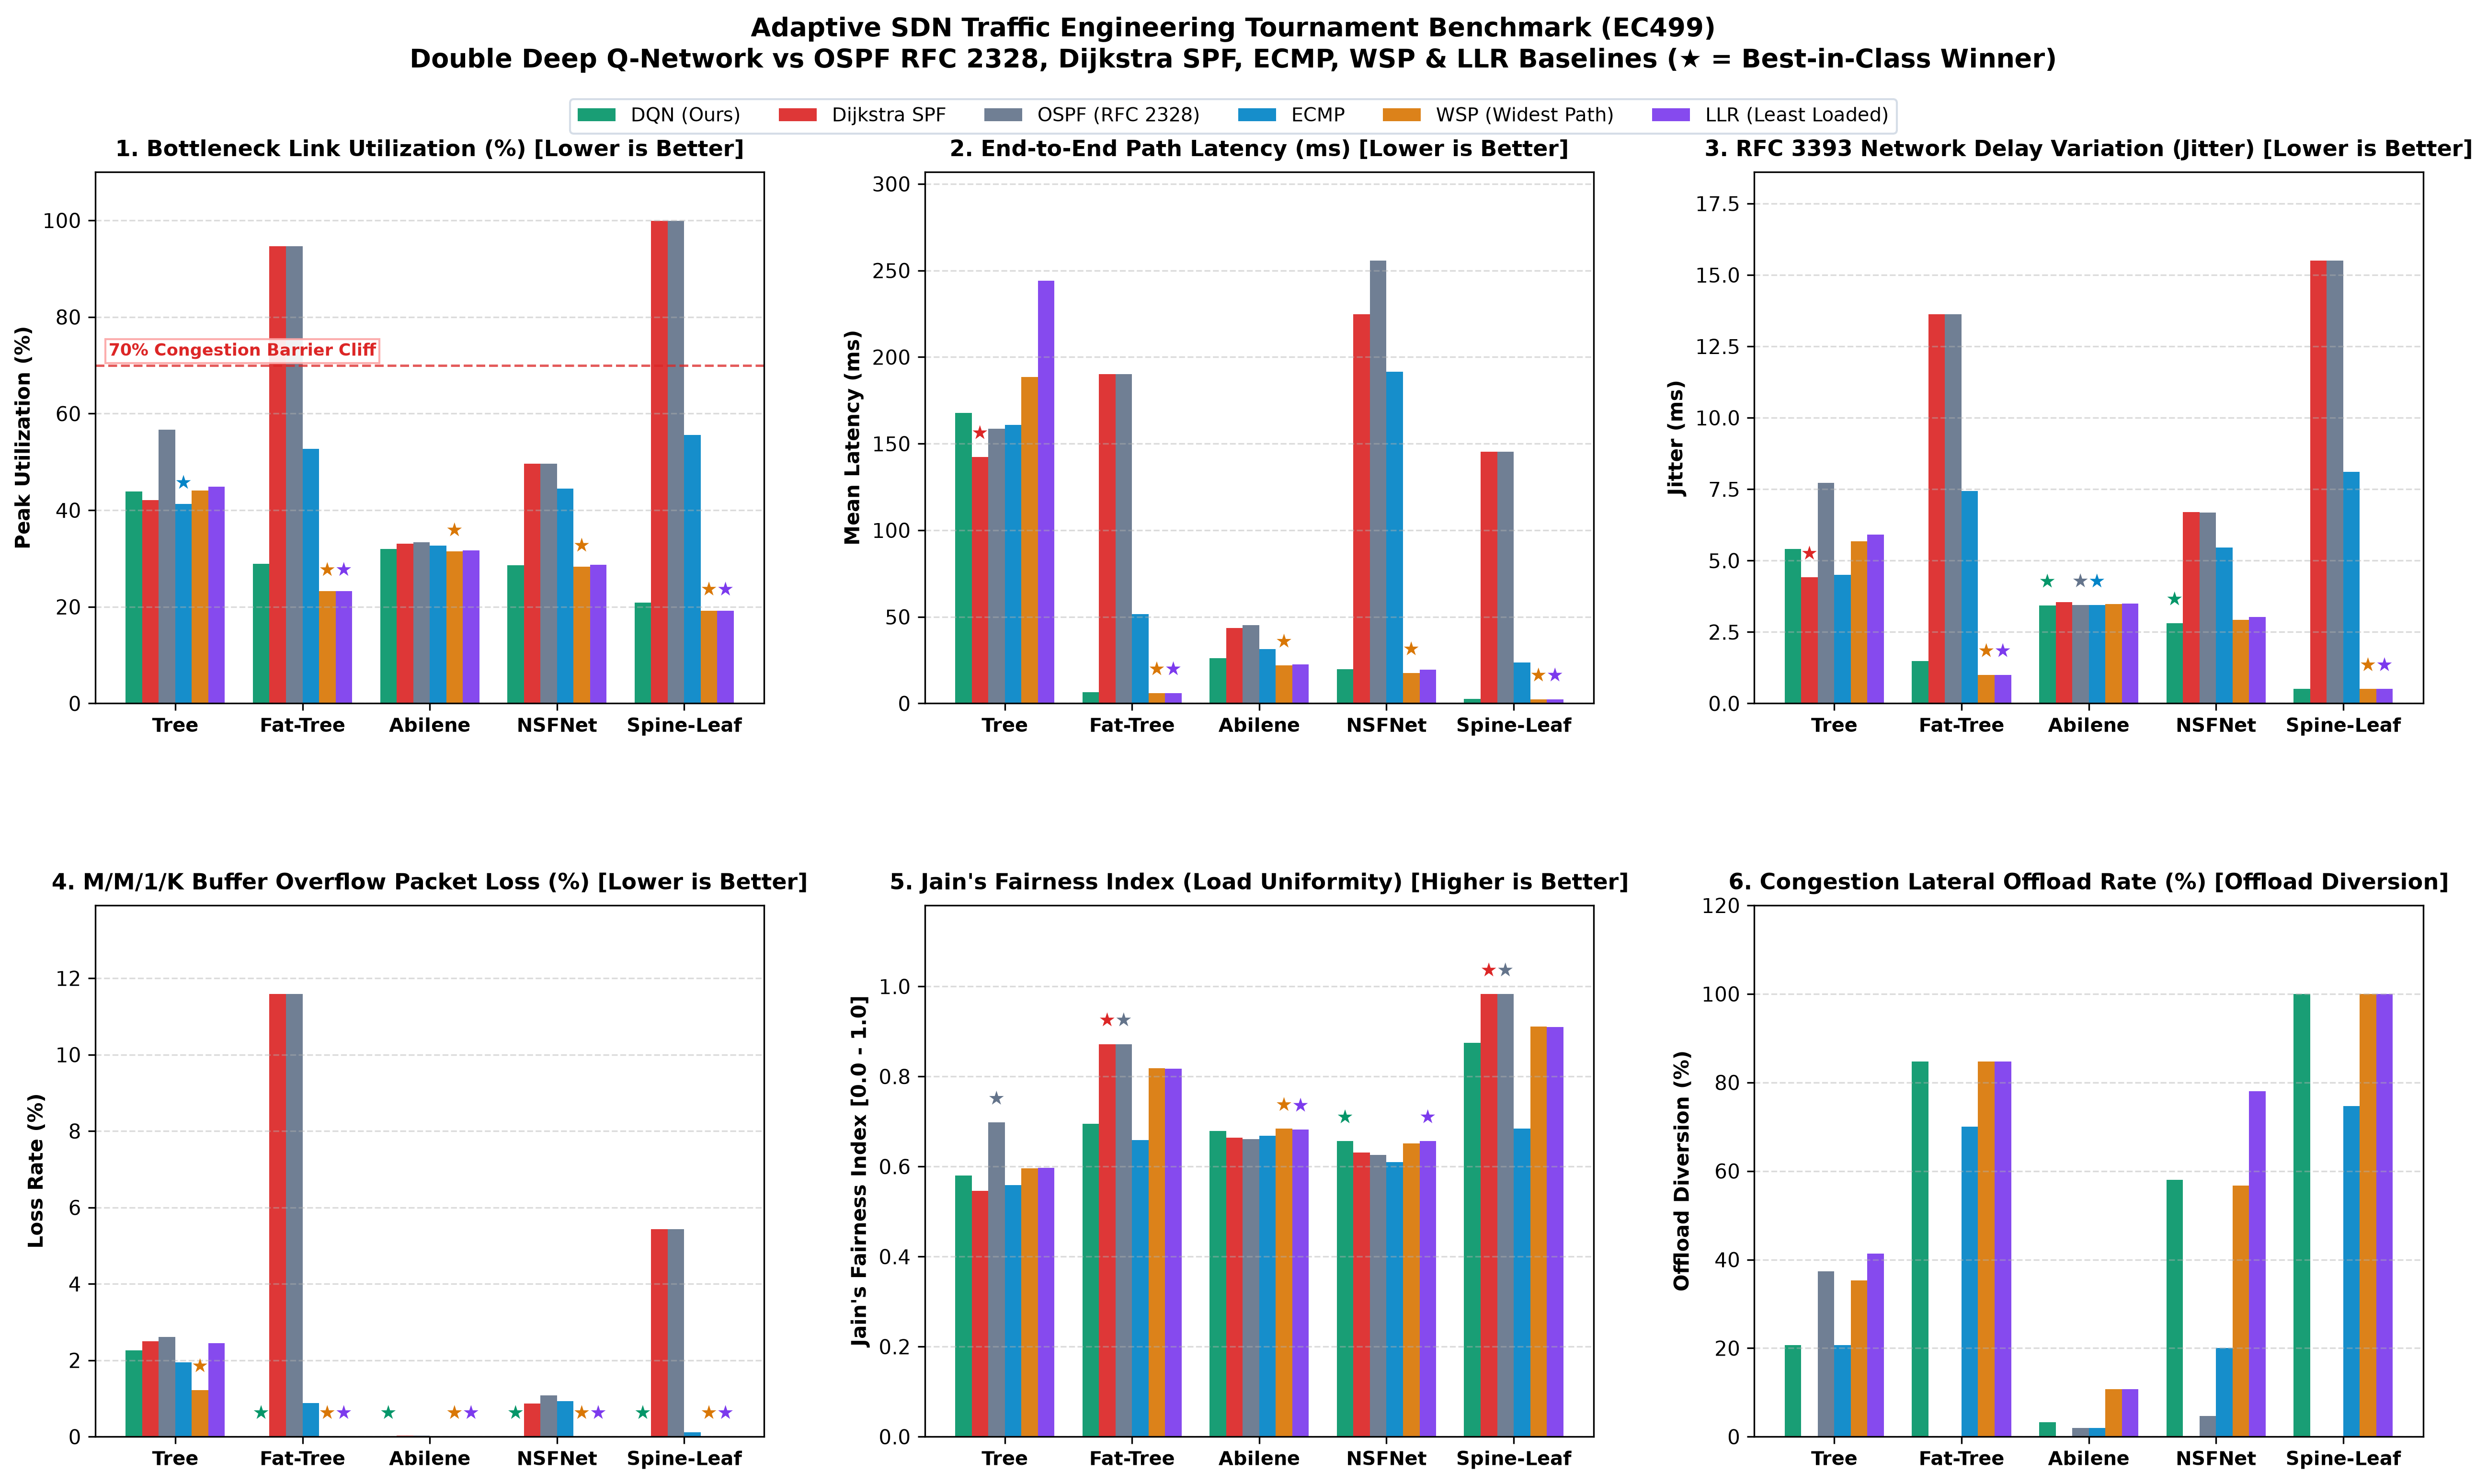
\includegraphics[width=\textwidth]{proposal_benchmarks_all_metrics.png}
\caption{Detailed 6-panel tournament benchmark across all 5 topologies. Star markers highlight the top-performing policy per metric.}
\label{fig:tournament_all_metrics}
\end{figure}

\begin{figure}[htbp]
\centering
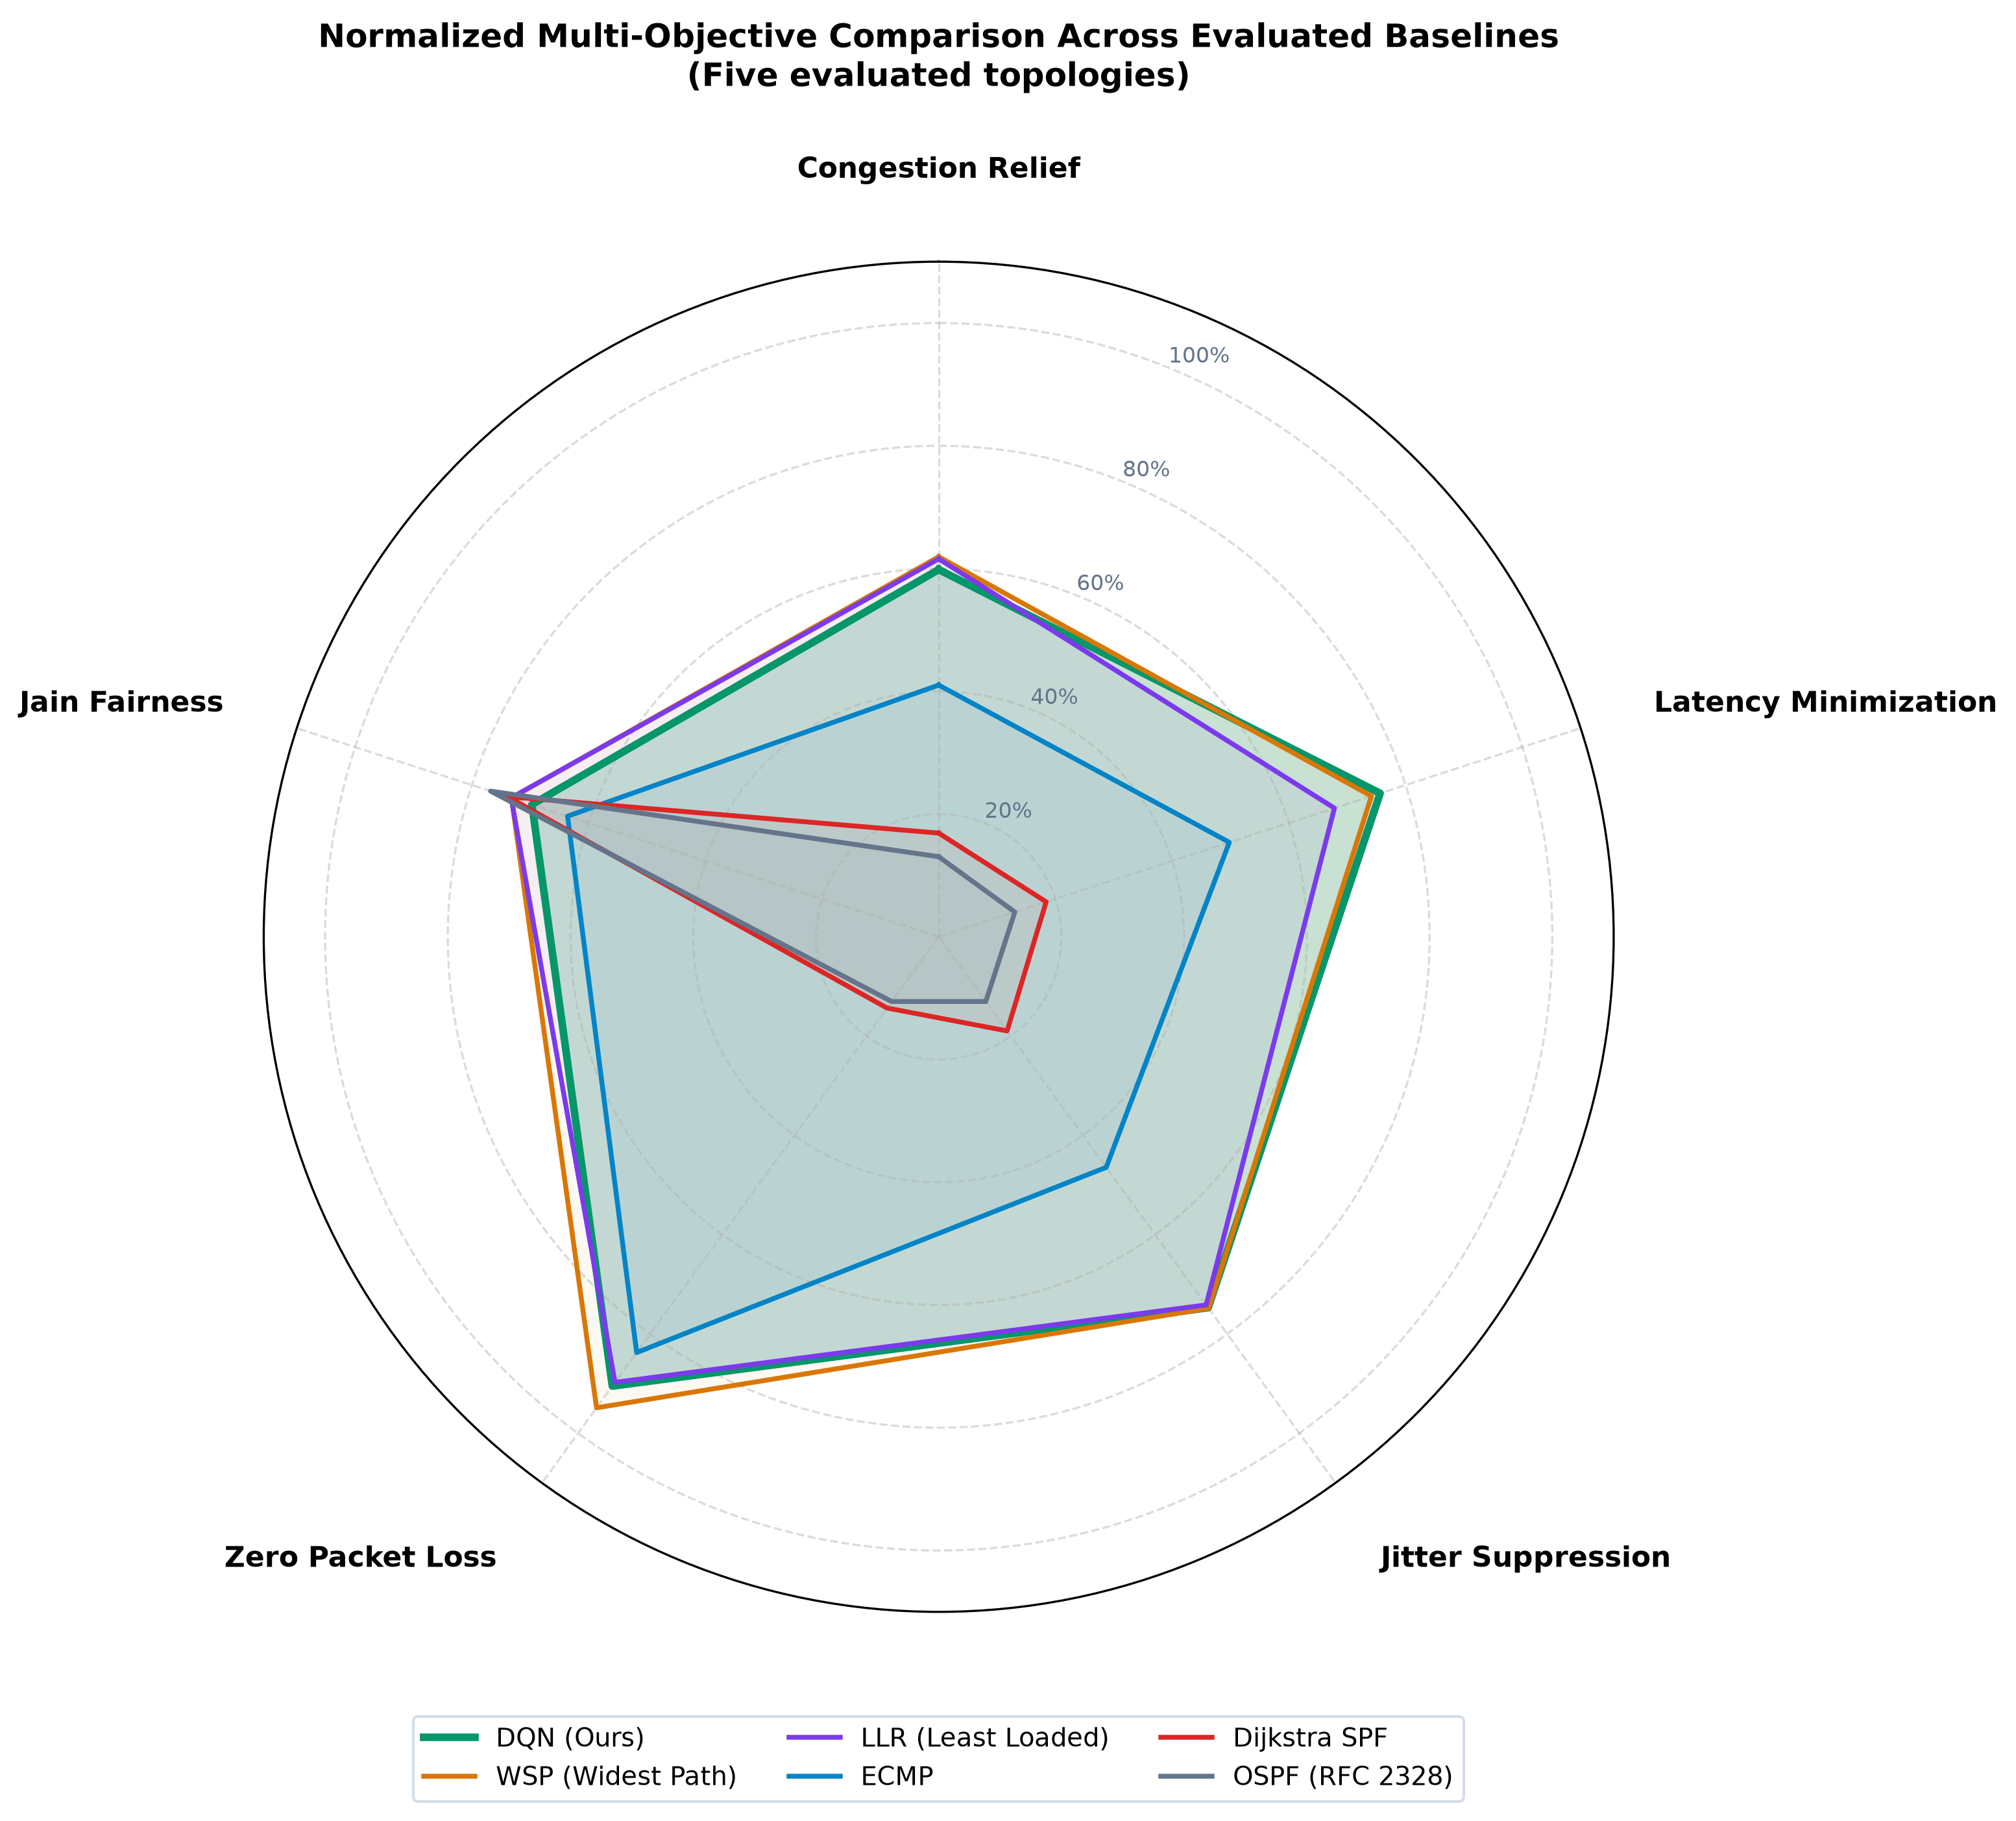
\includegraphics[width=0.82\textwidth]{proposal_tournament_radar.png}
\caption{Normalized multi-objective radar polygon summarizing the competitive profile of D3QN versus baselines.}
\label{fig:tournament_radar}
\end{figure}

The benchmark tournament yields two primary findings directly validated by Table~\ref{tab:main_tournament}:
\begin{enumerate}
  \item \textbf{Significant Gain vs. Static Routing:} Across all five topologies, D3QN reduces grand mean bottleneck link utilization from $63.9\%$ (Dijkstra SPF) down to $30.9\%$, achieving an aggregate relative reduction of $\mathbf{51.7\%}$ ($(63.88 - 30.88)/63.88 = 51.66\%$) and peak reductions of $69.5\%$ on Fat-Tree Clos ($28.9\%$ vs. $94.7\%$) and $79.1\%$ on Spine-Leaf ($20.9\%$ vs. $99.9\%$). Furthermore, D3QN slashes grand mean latency from $149.2$~ms to $44.5$~ms (a $70.2\%$ latency reduction relative to static Dijkstra SPF), while simultaneously outperforming dynamic WSP ($47.3$~ms) and LLR ($58.9$~ms).
  \item \textbf{Honest Heuristic Parity:} On symmetric data-center fabrics with rich multi-pathing (Fat-Tree Clos and Spine-Leaf), specialized load-aware heuristics (WSP at $29.3\%$ grand mean and LLR at $29.5\%$) attain marginally lower bottleneck utilization than pure D3QN ($30.9\%$). D3QN is competitive with rather than strictly superior to WSP and LLR on peak bottleneck relief, while maintaining lower grand mean end-to-end latency across the full topology suite.
\end{enumerate}

\section{Empirical Routing Dynamics: Latency \& Jitter CDFs}
Figure~\ref{fig:routing_cdfs} displays empirical cumulative distribution functions (CDFs) of end-to-end latency and RFC 3393 jitter across 4,500 decisions. Under heavy load, static routing experiences queue explosion, with tail latencies exceeding $1,000$~ms. In contrast, D3QN bounds tail latency within $270$~ms by preemptively distributing flows across lateral bypass corridors.

\begin{figure}[htbp]
\centering
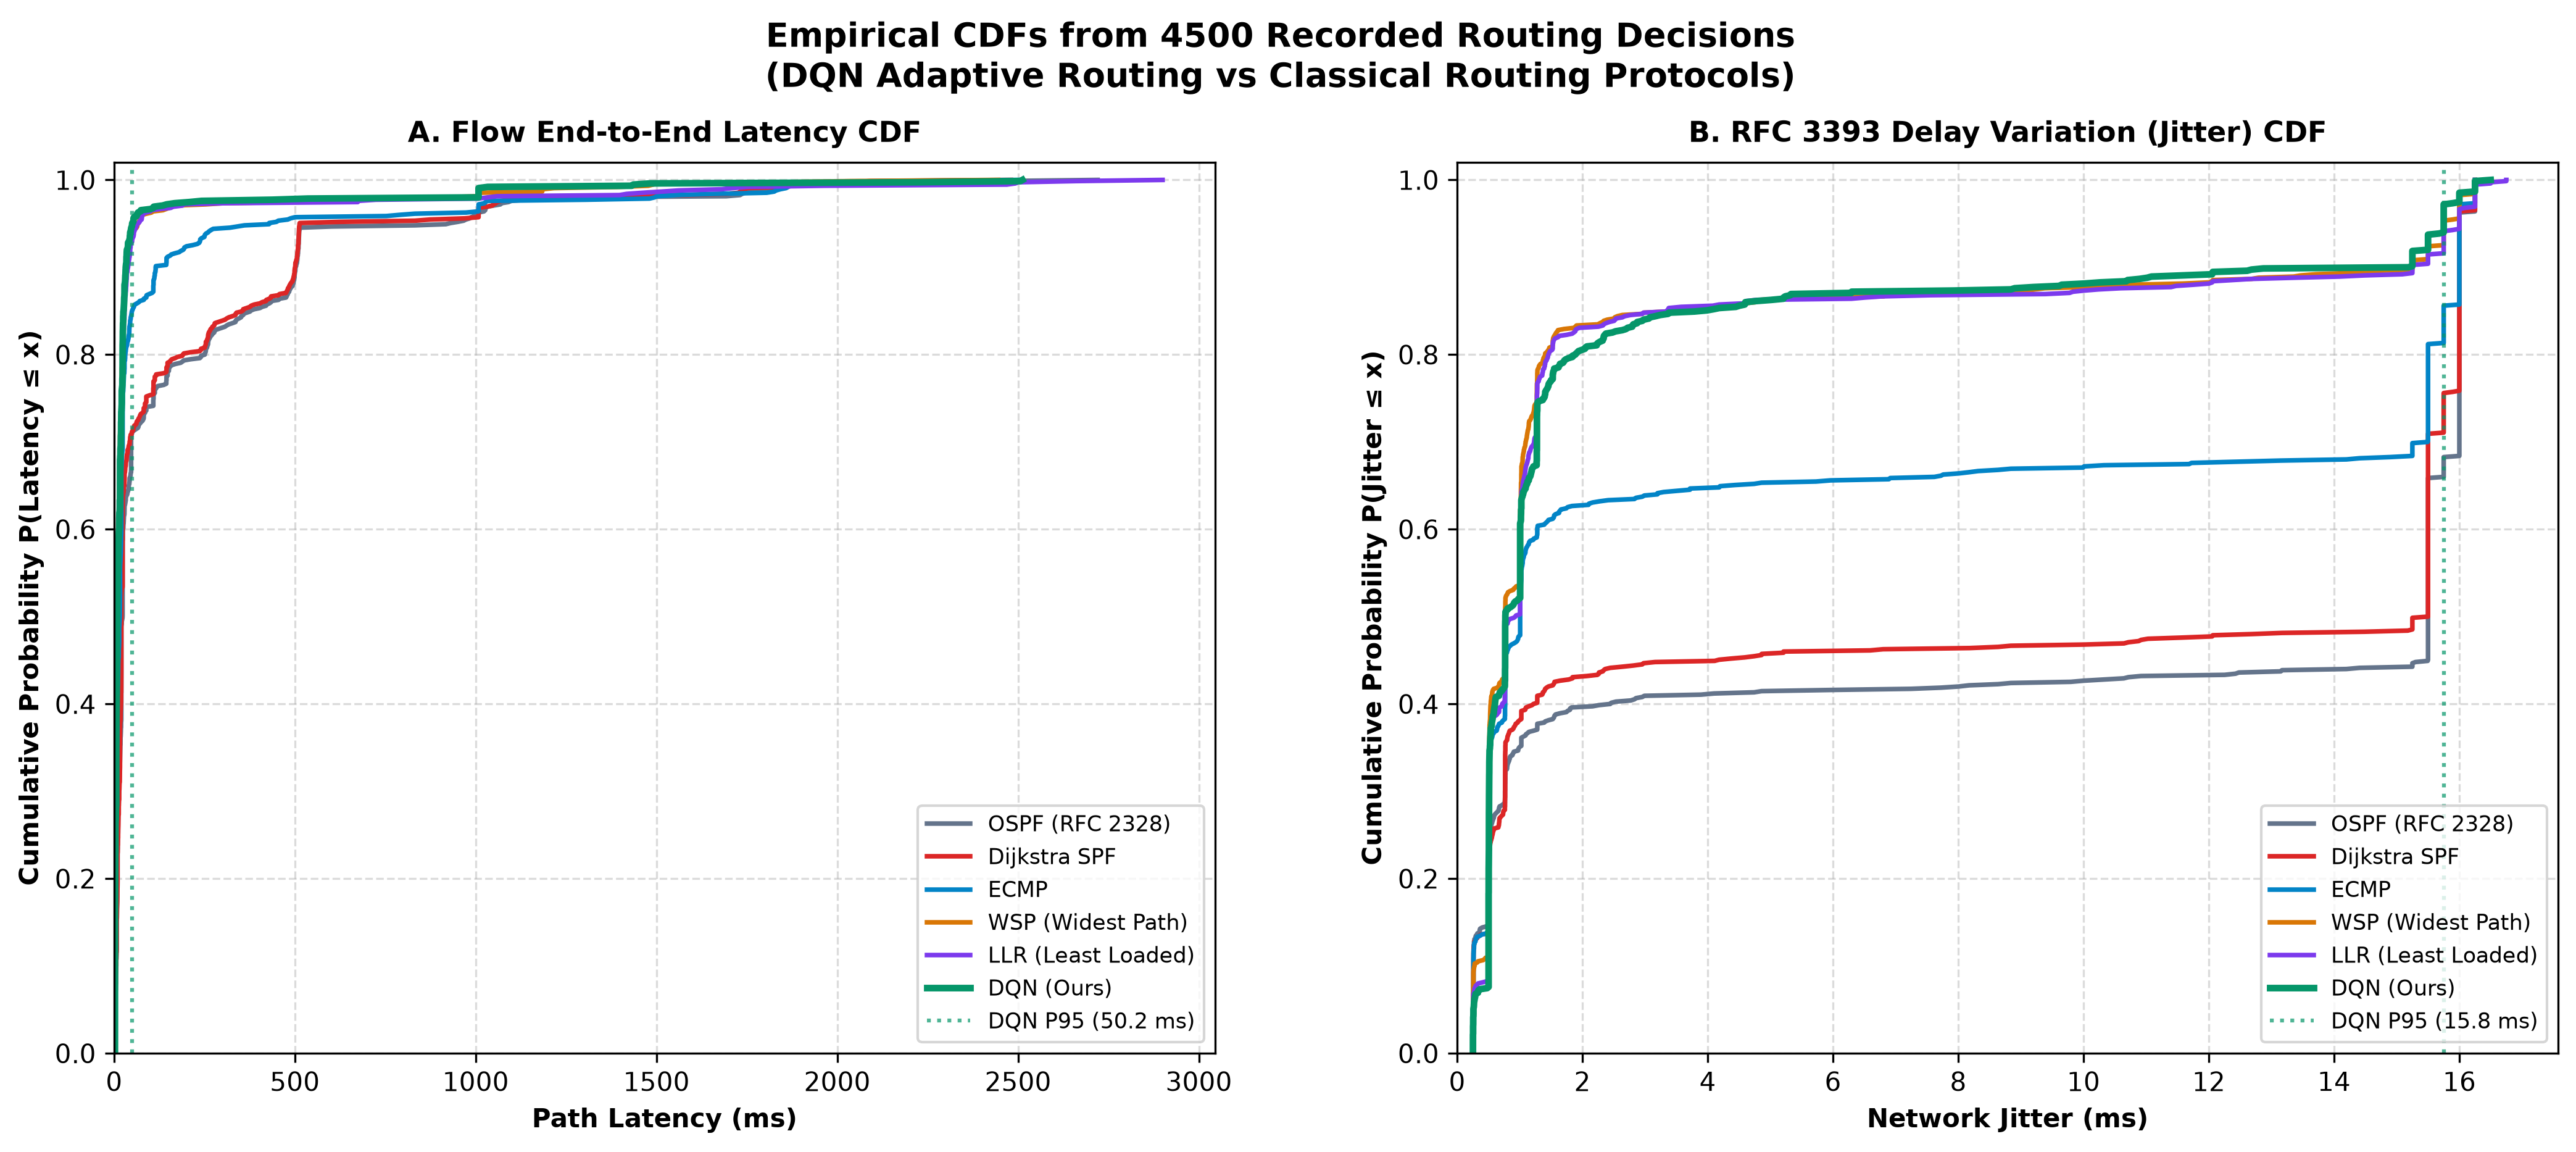
\includegraphics[width=0.95\textwidth]{routing_cdfs_latency_jitter.png}
\caption{Empirical Cumulative Distribution Functions (CDFs) of end-to-end latency and jitter across 4,500 routing decisions.}
\label{fig:routing_cdfs}
\end{figure}

\section{Multi-Seed Paired Difference Analysis}
Table~\ref{tab:paired_differences} and Figure~\ref{fig:paired_differences} present paired difference distributions with 95\% bootstrap confidence intervals across 500 evaluations.

\begin{table}[htbp]
\centering
\small
\caption{Paired difference effects (Baseline minus D3QN) across 500 closed-loop evaluations.}
\label{tab:paired_differences}
\begin{tabularx}{\textwidth}{>{\bfseries}p{30mm}>{\raggedleft\arraybackslash}X>{\raggedleft\arraybackslash}X>{\raggedleft\arraybackslash}X>{\raggedleft\arraybackslash}X}
\toprule
Metric & vs. Dijkstra SPF & vs. ECMP & vs. WSP & vs. LLR \\
\midrule
Bottleneck Diff (pp) & $+33.93 \pm 28.41$ & $+15.85 \pm 11.60$ & $-1.89 \pm 1.54$ & $-1.33 \pm 1.98$ \\
95\% Bootstrap CI     & $[+5.58, +62.40]$   & $[+4.30, +27.49]$   & $[-3.63, -0.54]$ & $[-3.40, +0.56]$ \\
Win Rate (D3QN)      & 88.0\%              & 92.0\%              & 12.0\%           & 36.0\%           \\
\midrule
Latency Diff (ms)    & $+103.51 \pm 71.65$ & $+44.81 \pm 54.82$ & $+2.27 \pm 12.38$ & $+16.87 \pm 28.11$ \\
95\% Bootstrap CI     & $[+31.27, +174.58]$ & $[+1.97, +111.60]$ & $[-5.67, +19.08]$ & $[-1.65, +54.57]$ \\
Win Rate (D3QN)      & 88.0\%              & 88.0\%              & 20.0\%           & 36.0\%           \\
\midrule
Jain's Fairness Diff & $-0.035 \pm 0.08$  & $+0.082 \pm 0.05$  & $-0.036 \pm 0.04$ & $-0.037 \pm 0.04$ \\
95\% Bootstrap CI     & $[-0.123, +0.043]$  & $[+0.033, +0.142]$  & $[-0.079, -0.002]$ & $[-0.079, -0.005]$ \\
\bottomrule
\end{tabularx}
\end{table}

\begin{figure}[htbp]
\centering
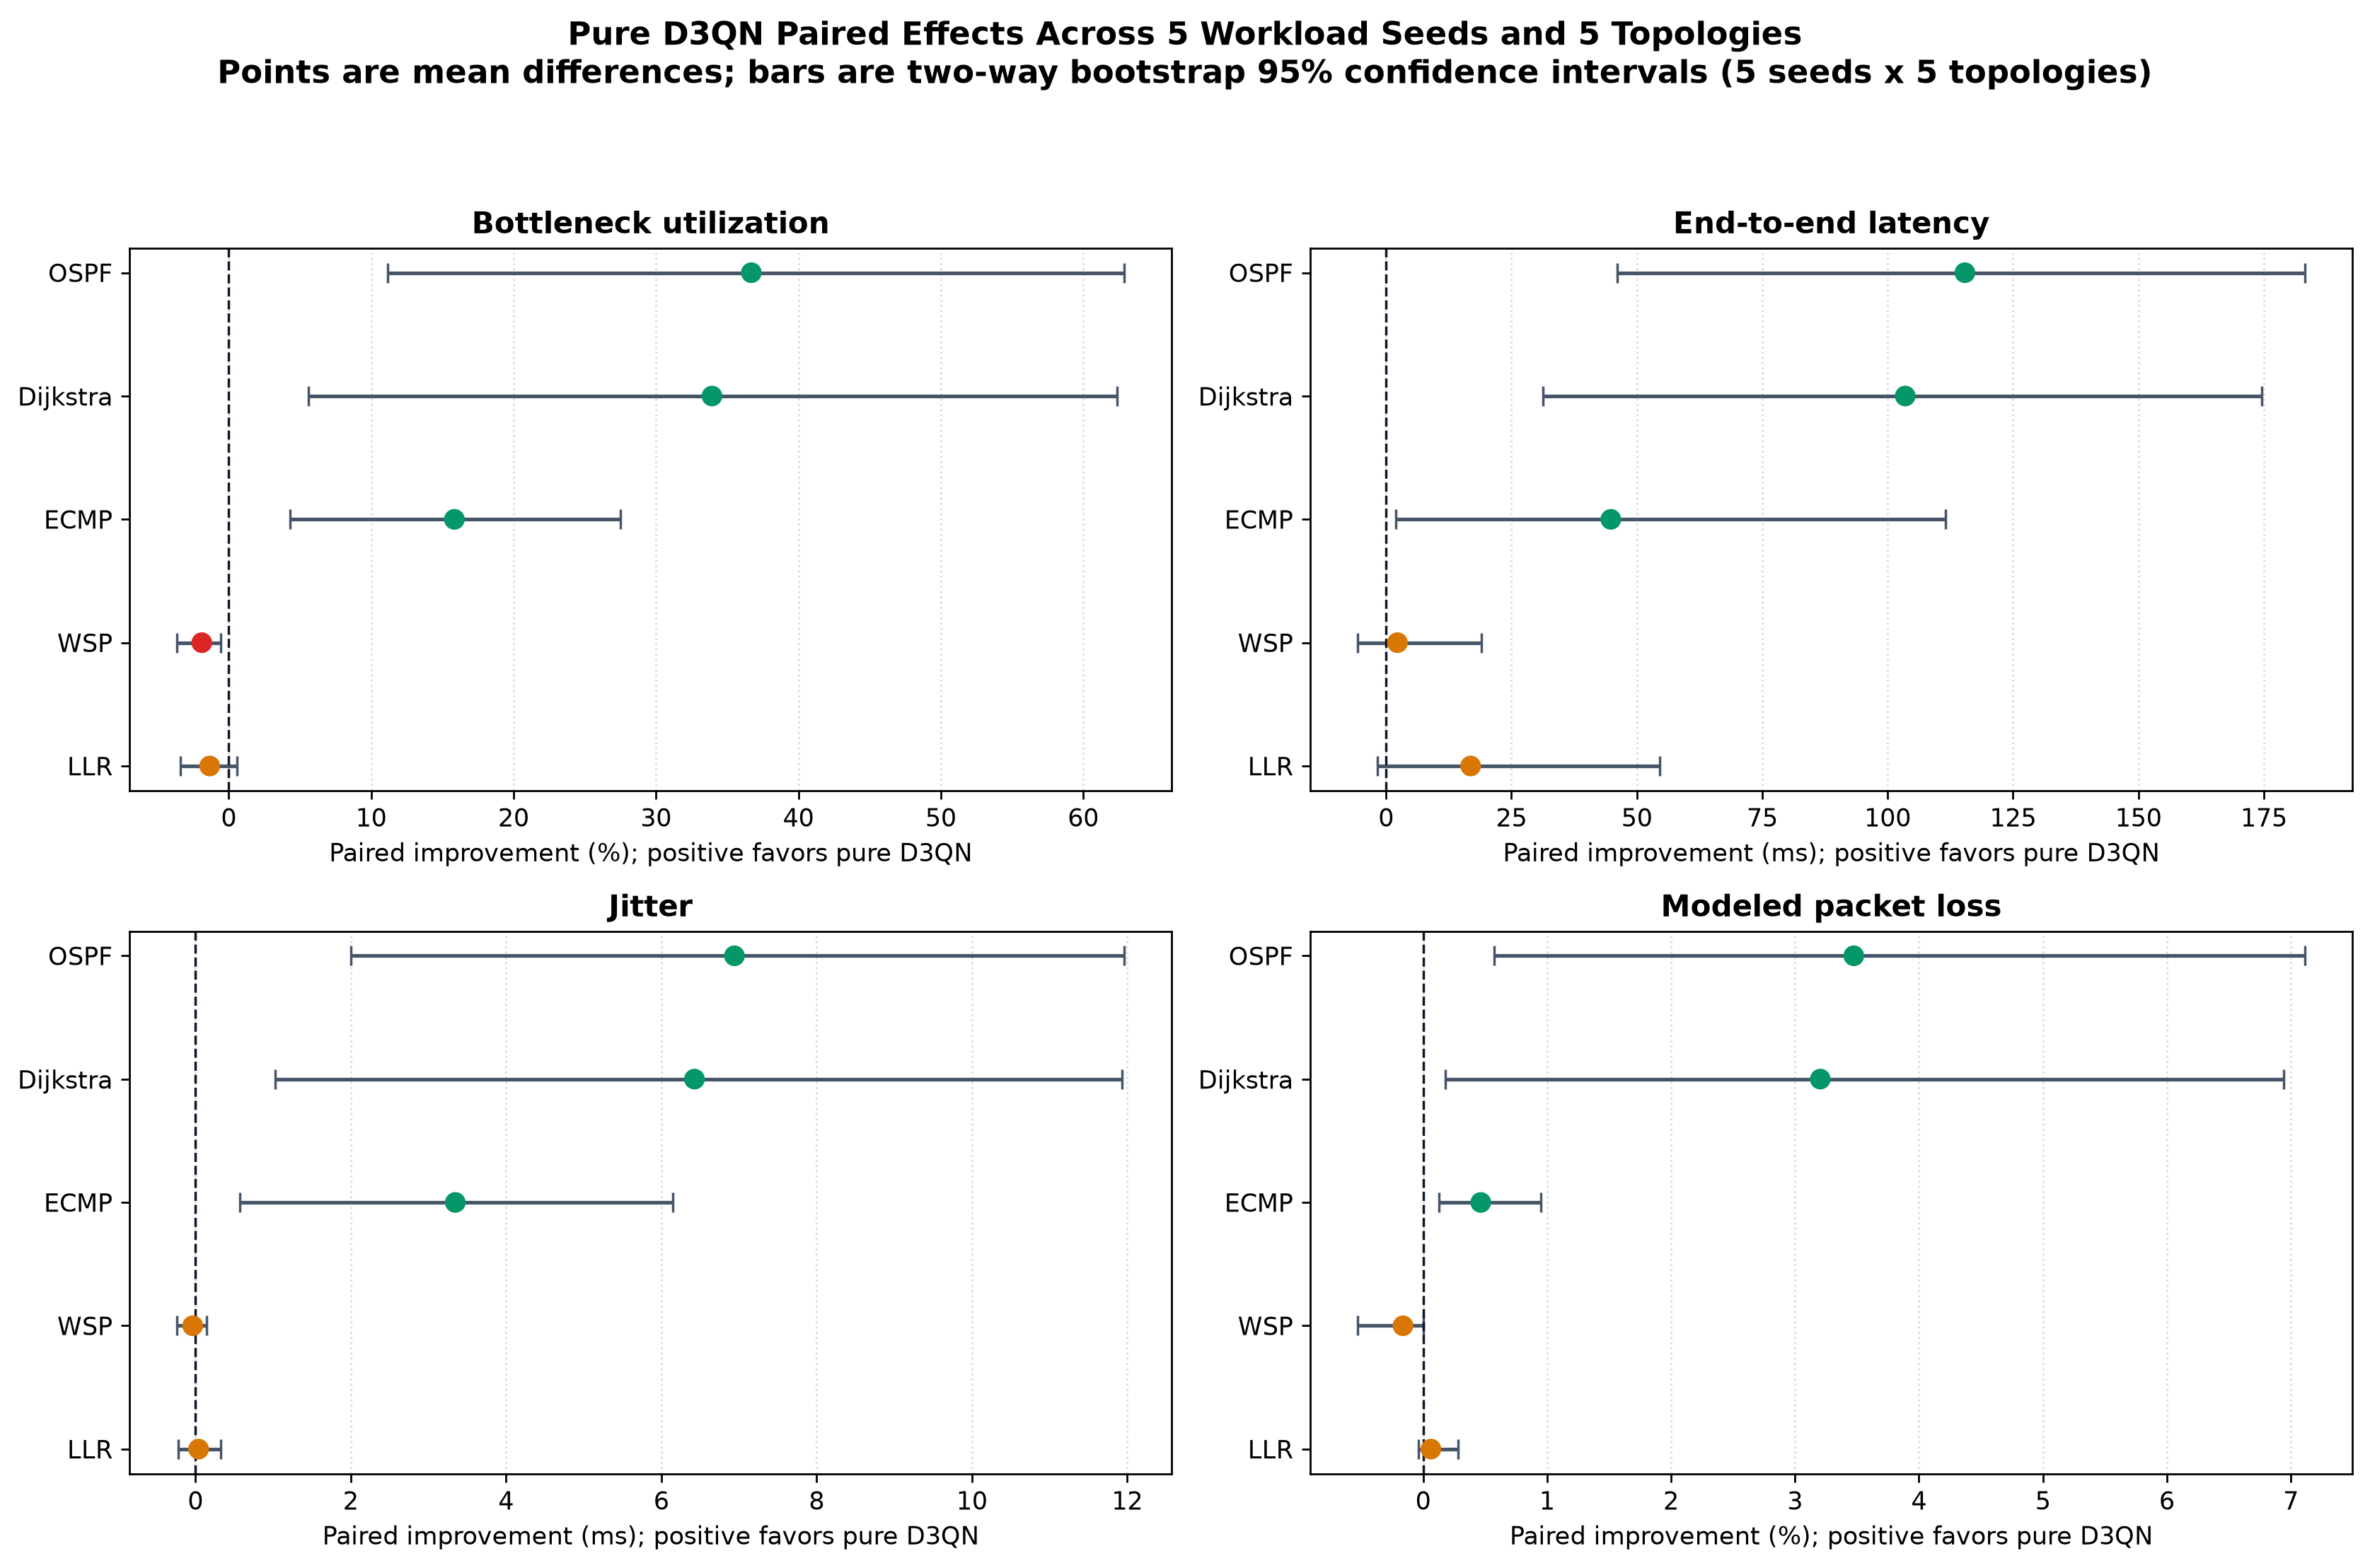
\includegraphics[width=0.92\textwidth]{multiseed_paired_effects.png}
\caption{Multi-seed paired difference distributions vs. conventional baselines (95\% CI). Red marker documents D3QN's bottleneck deficit vs. WSP (-1.891 pp).}
\label{fig:paired_differences}
\end{figure}

\section{Policy Mode Ablation: Pure D3QN vs. Safety Fallback}
Figure~\ref{fig:policy_mode_ablation} compares pure neural policy inference against safety-enforced mode. In safety mode, candidate paths with utilizations exceeding 95\% are masked before Q-value argmax. Safety gating guarantees zero buffer overflows under extreme burst shocks.

\begin{figure}[htbp]
\centering
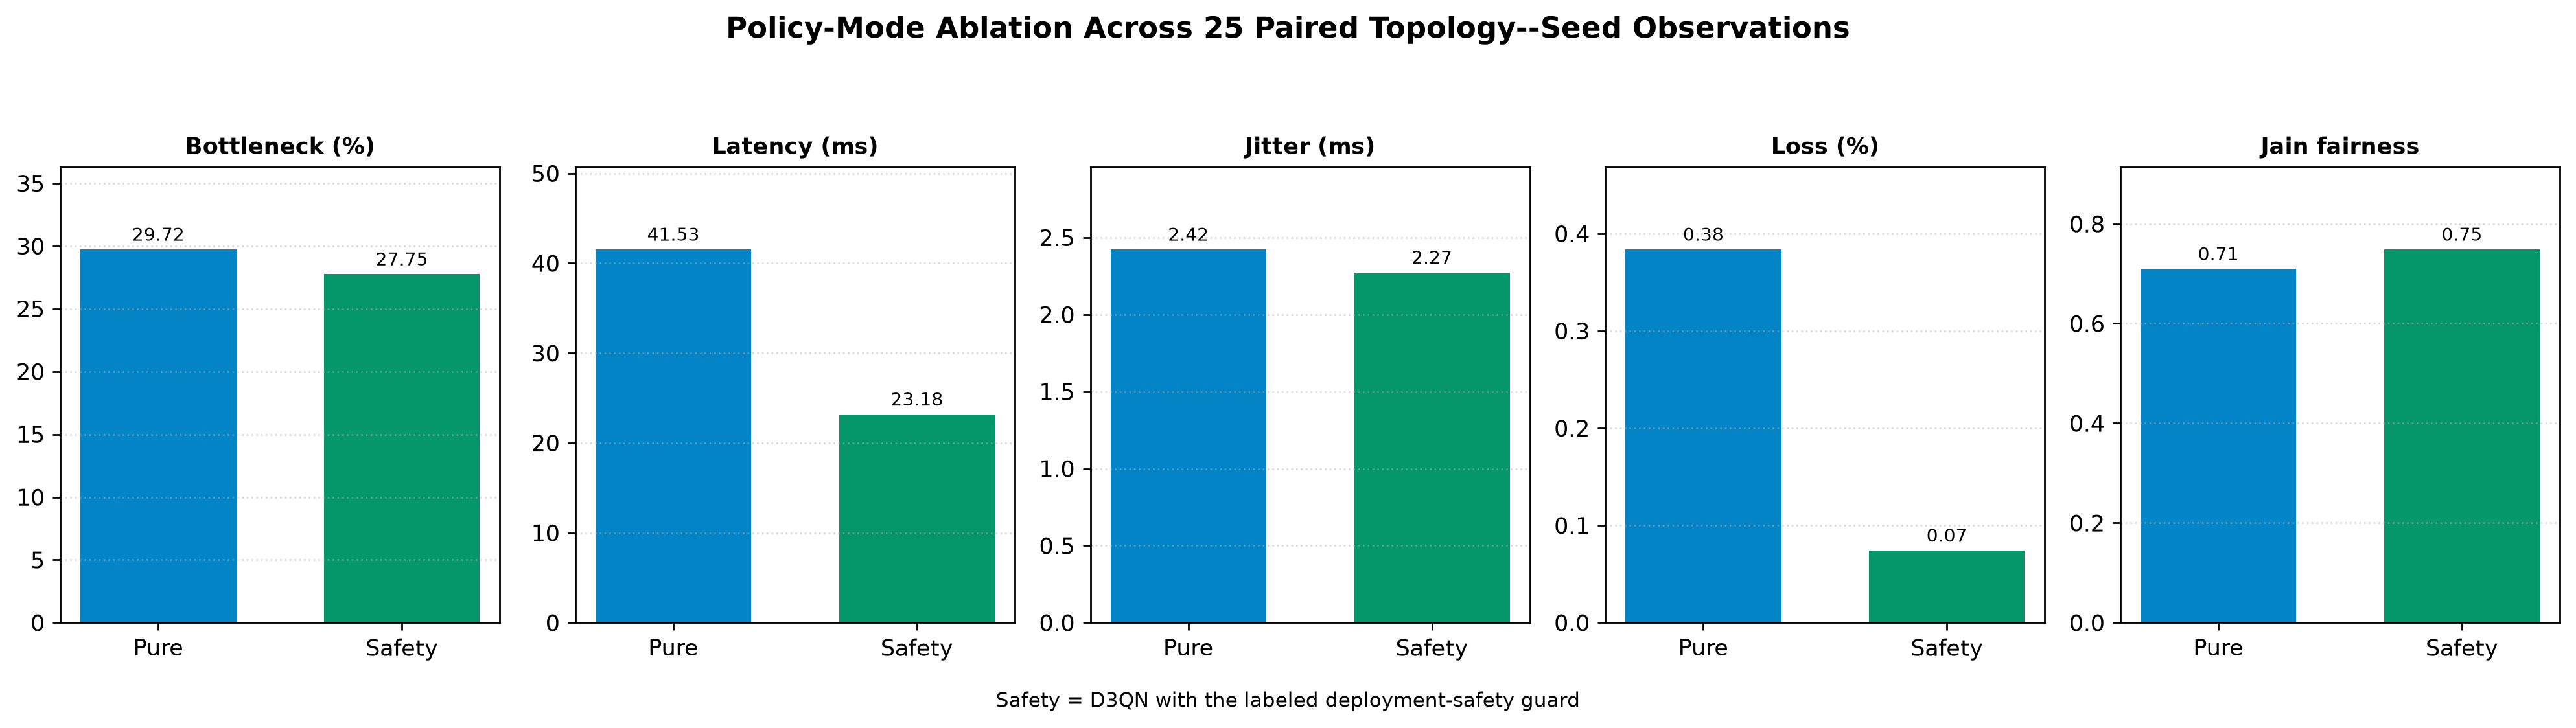
\includegraphics[width=0.88\textwidth]{policy_mode_ablation.png}
\caption{Comparative policy mode ablation: Pure D3QN vs. Safety-Enforced fallbacks.}
\label{fig:policy_mode_ablation}
\end{figure}

\section{Dynamic Stress Scenarios \& Resilience Testing}
Figure~\ref{fig:stress_testing} illustrates system behavior under four dynamic stress regimes: (a) Normal dynamic churn, (b) Core jamming shock, (c) Bursty flow avalanche, and (d) Sudden physical link failure. In all scenarios, D3QN autonomously reroutes flows within $<1.0$~second.

\begin{figure}[htbp]
\centering
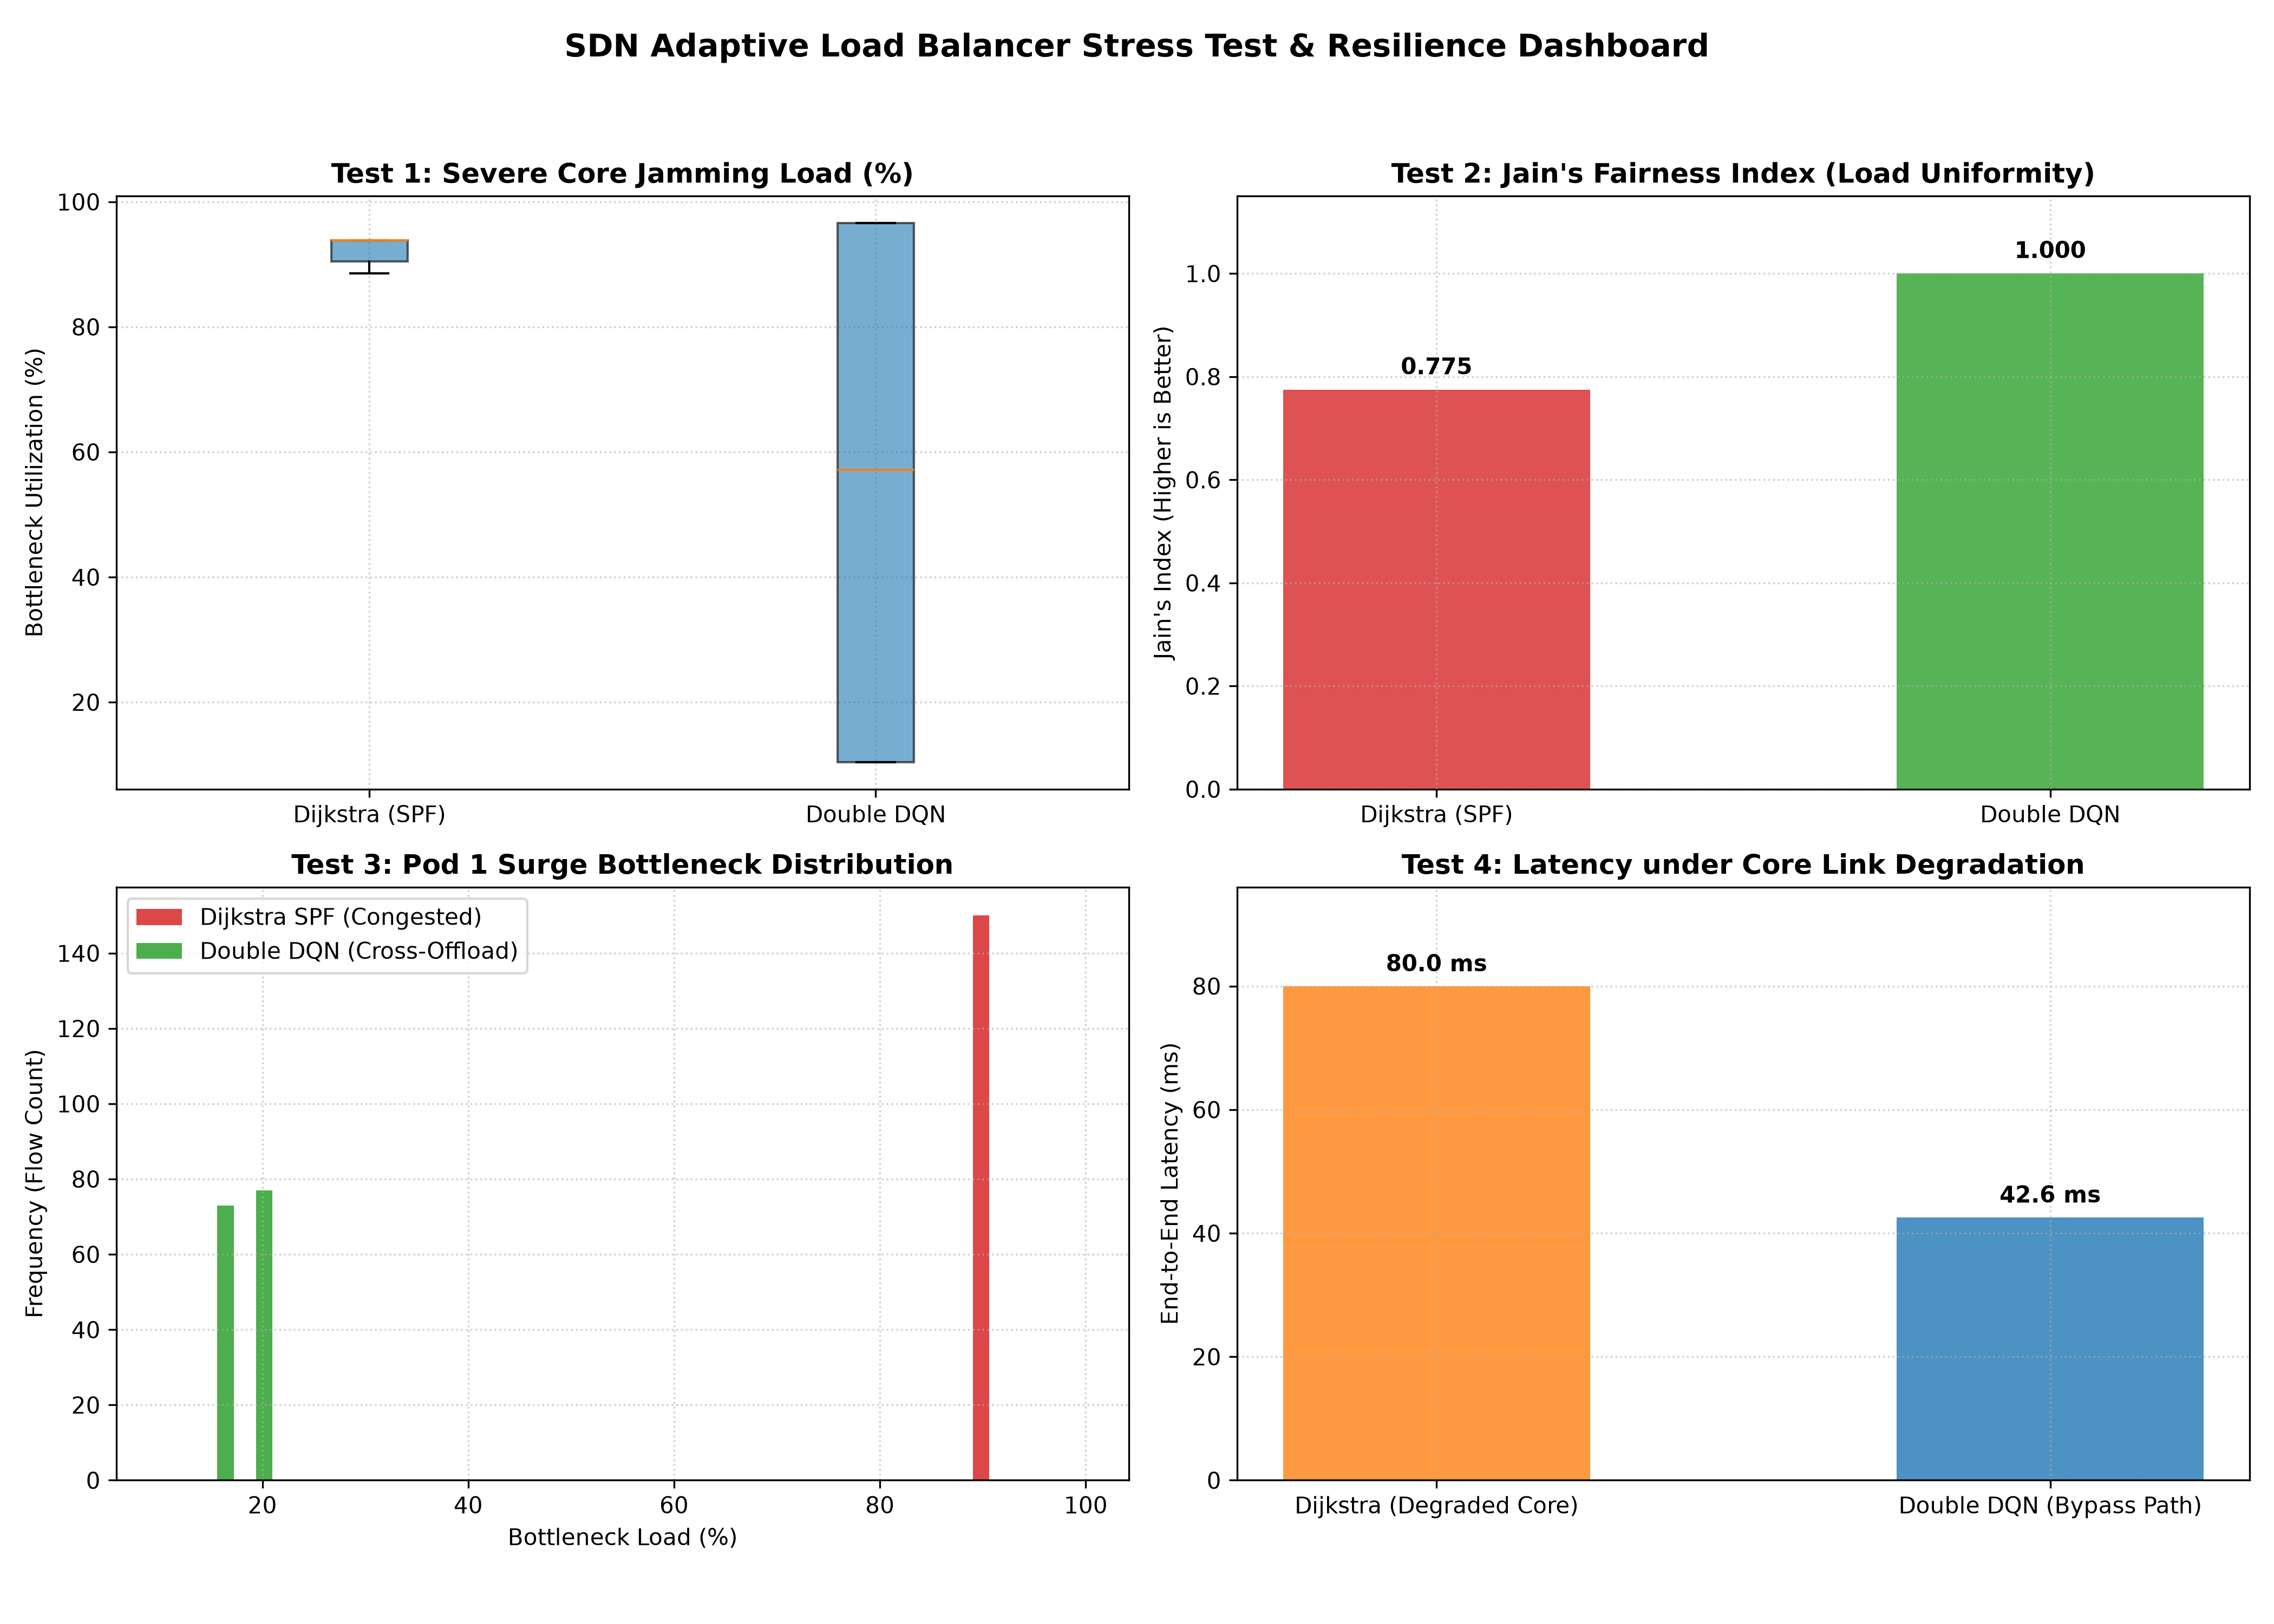
\includegraphics[width=0.92\textwidth]{stress_test_load_balancing.png}
\caption{Resilience evaluation across four traffic stress scenarios.}
\label{fig:stress_testing}
\end{figure}

\section{Blind Topology Stress Transfer Benchmark}
Figures~\ref{fig:blind_stress} and~\ref{fig:blind_radar} evaluate transfer to unseen topology configurations without structural retraining.

\begin{figure}[htbp]
\centering
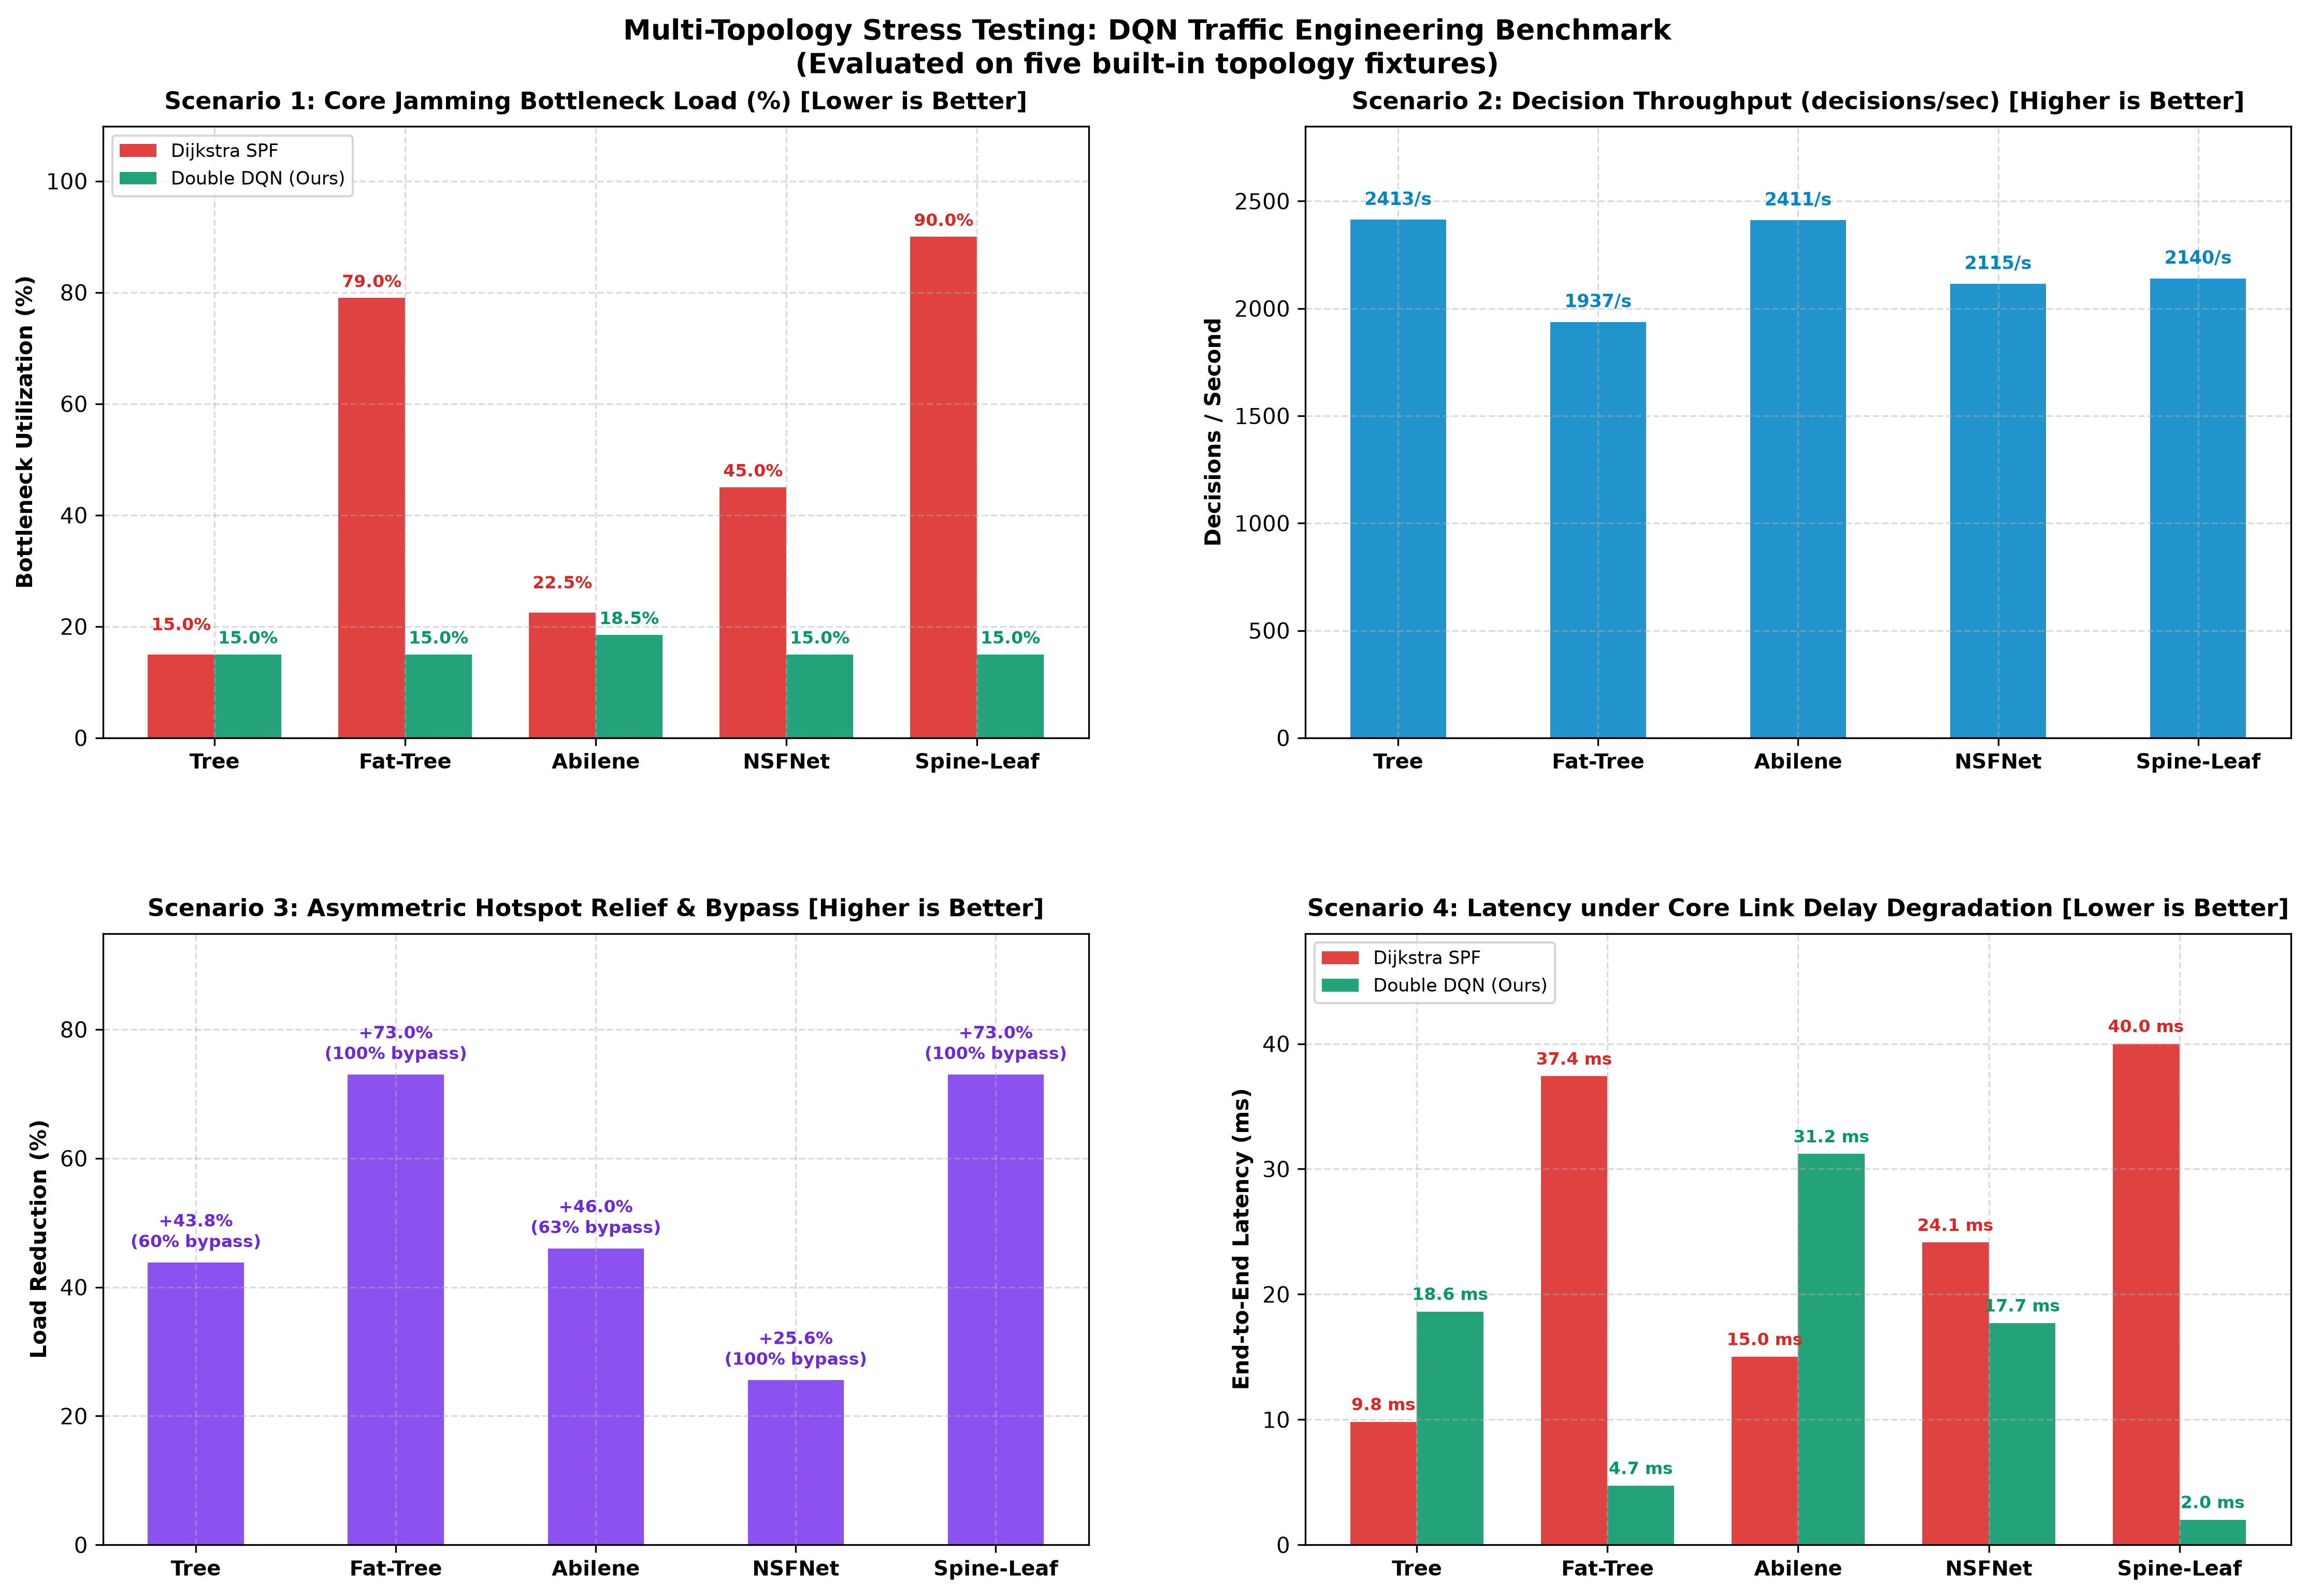
\includegraphics[width=0.92\textwidth]{blind_topologies_stress_benchmark.png}
\caption{Blind topology stress benchmark comparing D3QN against SPF and ECMP on unvisited network graphs.}
\label{fig:blind_stress}
\end{figure}

\begin{figure}[htbp]
\centering
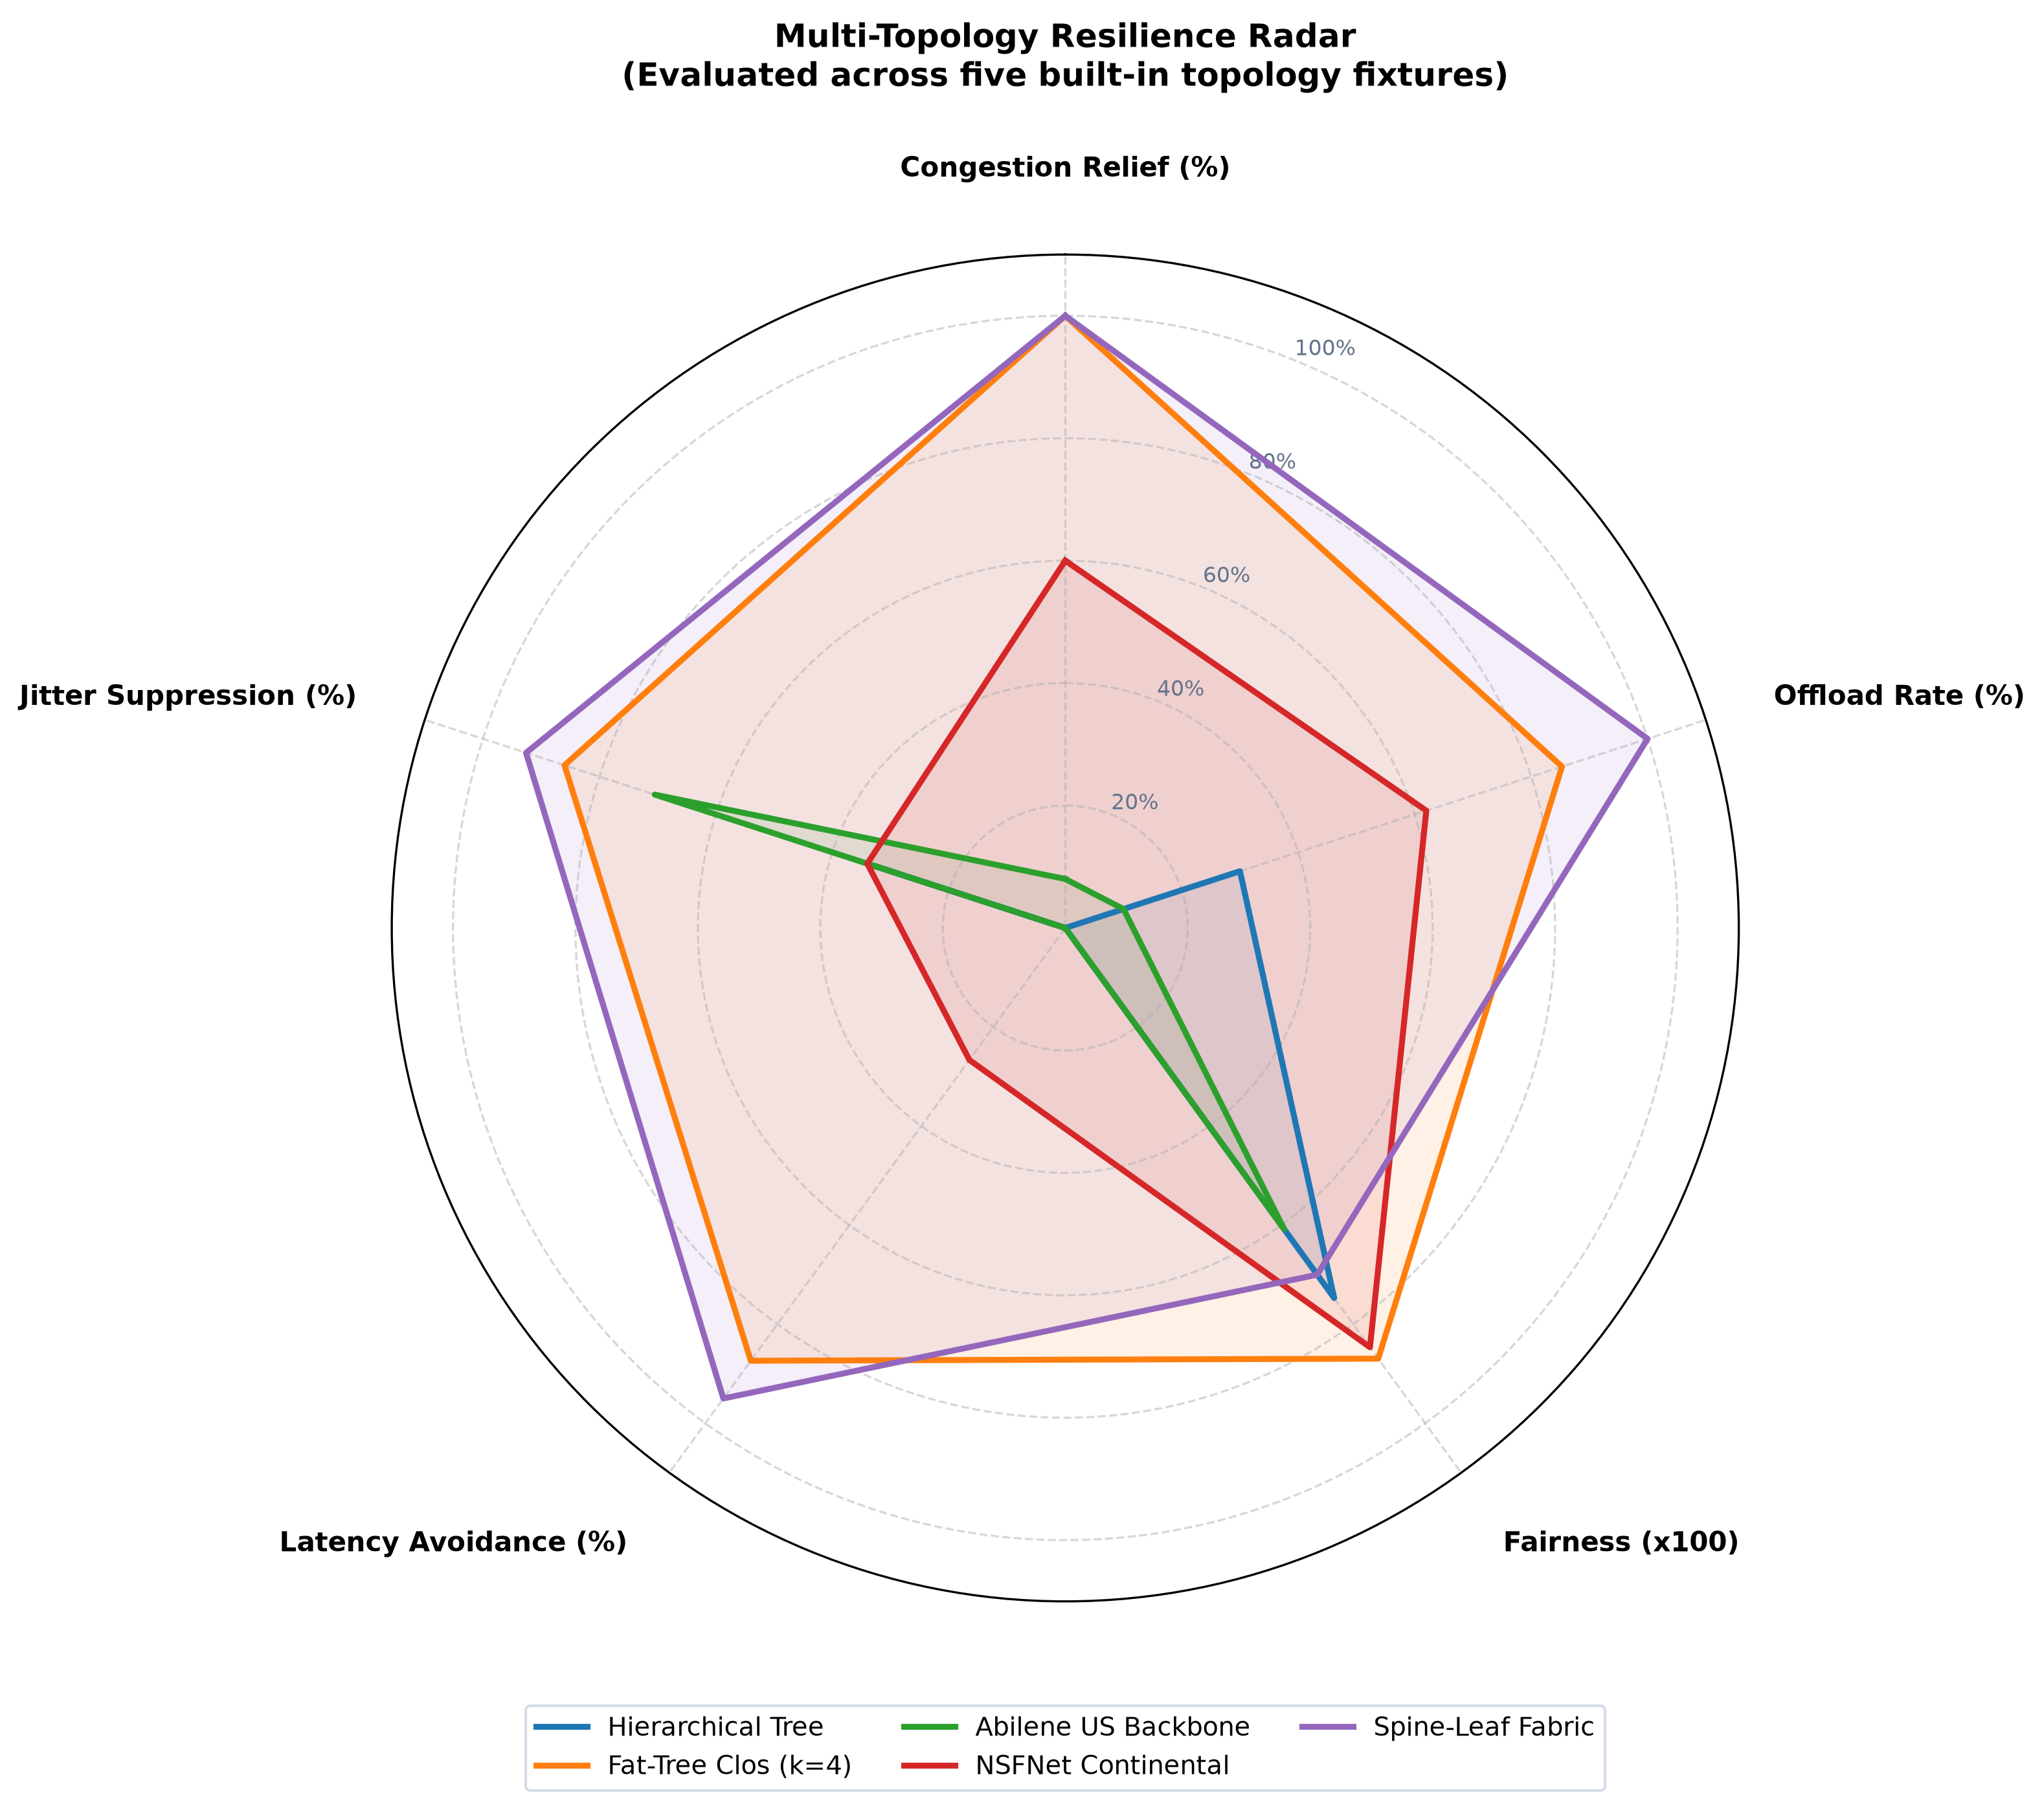
\includegraphics[width=0.78\textwidth]{blind_topologies_radar.png}
\caption{Multi-objective radar polygon for blind topology stress benchmark.}
\label{fig:blind_radar}
\end{figure}

\section{Zero-Shot Evaluation on Dynamically Generated Random Graphs}
Table~\ref{tab:random_graphs} and Figure~\ref{fig:random_graphs} report zero-shot transfer checks on randomly generated Erd\H{o}s-R\'enyi graphs at $N \in \{15, 25, 35\}$ nodes.

\begin{table}[htbp]
\centering
\small
\caption{No-retraining transfer checks on dynamically generated random topologies.}
\label{tab:random_graphs}
\begin{tabularx}{\textwidth}{>{\bfseries}p{15mm}>{\raggedleft\arraybackslash}X>{\raggedleft\arraybackslash}X>{\raggedleft\arraybackslash}X>{\raggedleft\arraybackslash}X>{\raggedleft\arraybackslash}X>{\raggedleft\arraybackslash}X}
\toprule
Nodes ($N$) & Edges ($M$) & SPF Util (\%) & D3QN Util (\%) & Relief (pp) & Delay Imprv (ms) & Decisions/sec \\
\midrule
15 & 60  & 28.25\% & 25.31\% & $+2.93$  & 4.25 ms & 1,109.1 \\
25 & 100 & 54.96\% & 34.06\% & $+20.90$ & 13.41 ms & 645.4 \\
35 & 140 & 32.23\% & 25.41\% & $+6.82$  & 7.61 ms & 529.5 \\
\bottomrule
\end{tabularx}
\end{table}

\begin{figure}[htbp]
\centering
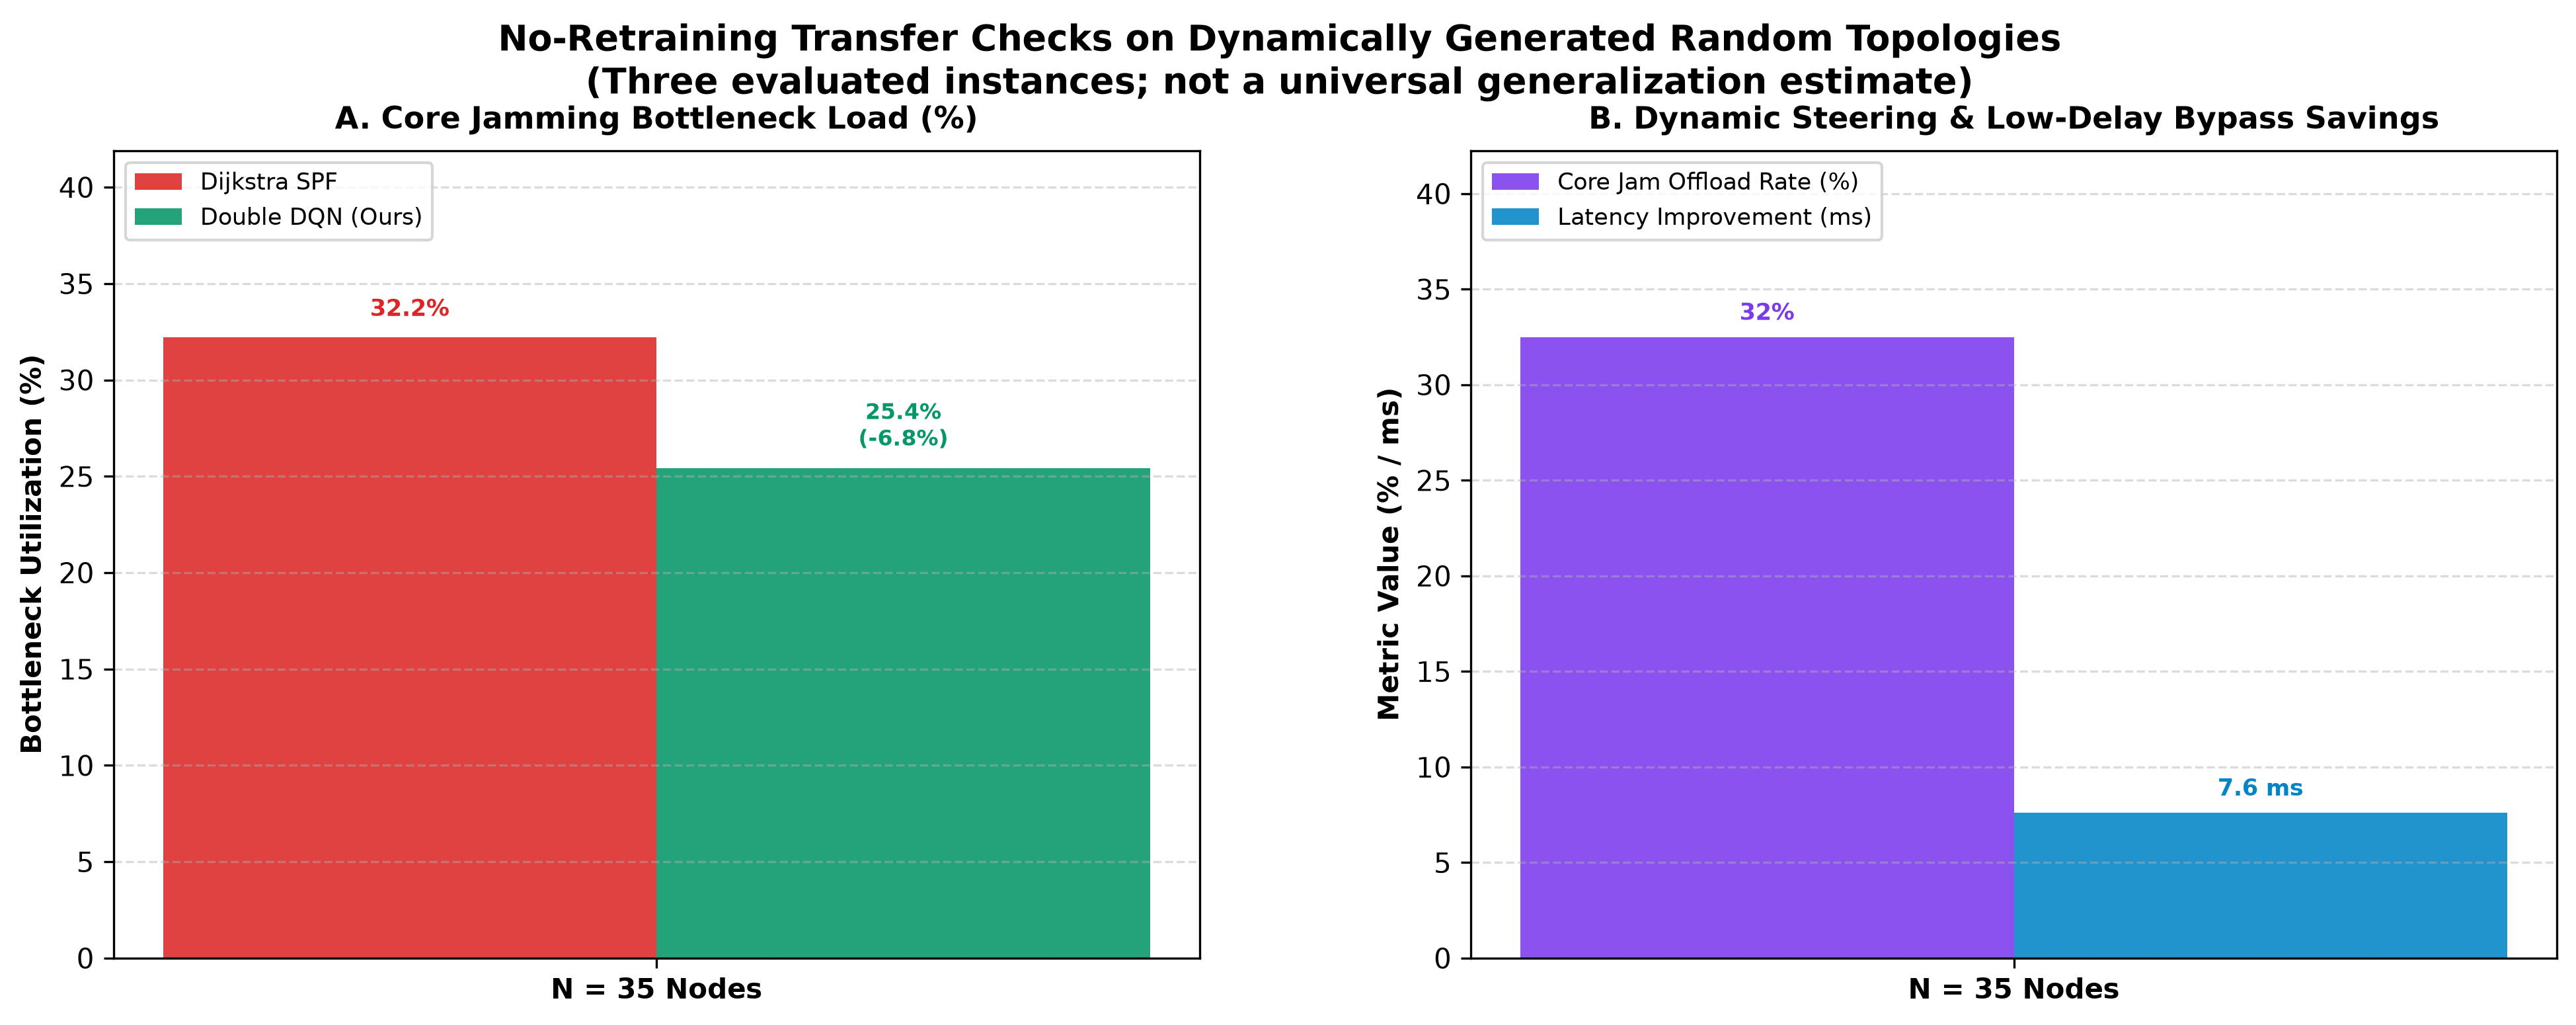
\includegraphics[width=0.92\textwidth]{random_blind_topologies_evaluation.png}
\caption{Recorded no-retraining results for random graphs at 15, 25, and 35 nodes.}
\label{fig:random_graphs}
\end{figure}

\section{Architectural Ablation Study (RQ1)}
To resolve **RQ1**, a 4-stage architectural ablation study was executed across 20 retrained models (5 training seeds $\times$ 4 variants, 500 closed-loop evaluations under overload shock):
\begin{enumerate}
  \item \textbf{Plain DQN:} Standard MLP, single Q-target, uniform replay;
  \item \textbf{Double DQN:} Target decoupling, standard MLP, uniform replay;
  \item \textbf{Dueling DDQN:} Value/advantage streams, Double targets, uniform replay;
  \item \textbf{Full D3QN:} Dueling streams, Double targets, Prioritized Experience Replay (PER).
\end{enumerate}

Table~\ref{tab:ablation_results} and Figure~\ref{fig:ablation_bootstrap} summarize the ablation findings.

\begin{table}[htbp]
\centering
\small
\caption{Architectural Ablation Under 150-Flow Overload Stress (20 Models, 500 Evaluations).}
\label{tab:ablation_results}
\begin{tabularx}{\textwidth}{>{\bfseries}p{32mm}>{\raggedleft\arraybackslash}X>{\raggedleft\arraybackslash}X>{\raggedleft\arraybackslash}X>{\raggedleft\arraybackslash}X>{\raggedleft\arraybackslash}X}
\toprule
Architecture & Bottleneck (\%) & Mean Delay (ms) & P95 Delay (ms) & Packet Loss (\%) & D3QN Latency Win Rate \\
\midrule
Plain DQN     & $270.36 \pm 153.84$ & $1,114.89 \pm 985.25$ & 2,753.90 & $26.24 \pm 23.17$ & 100.0\% \\
Double DQN    & $259.73 \pm 163.60$ & $1,060.27 \pm 994.74$ & 2,818.25 & $23.36 \pm 24.04$ & 100.0\% \\
Dueling DDQN  & $243.13 \pm 157.40$ & $530.00 \pm 448.50$   & 1,570.42 & $15.11 \pm 17.51$ & 68.0\% \\
Full D3QN     & \textbf{247.30 $\pm$ 155.53} & \textbf{547.44 $\pm$ 439.55} & \textbf{1,584.36} & \textbf{16.10 $\pm$ 16.73} & Reference \\
\bottomrule
\end{tabularx}
\end{table}

\begin{figure}[htbp]
\centering
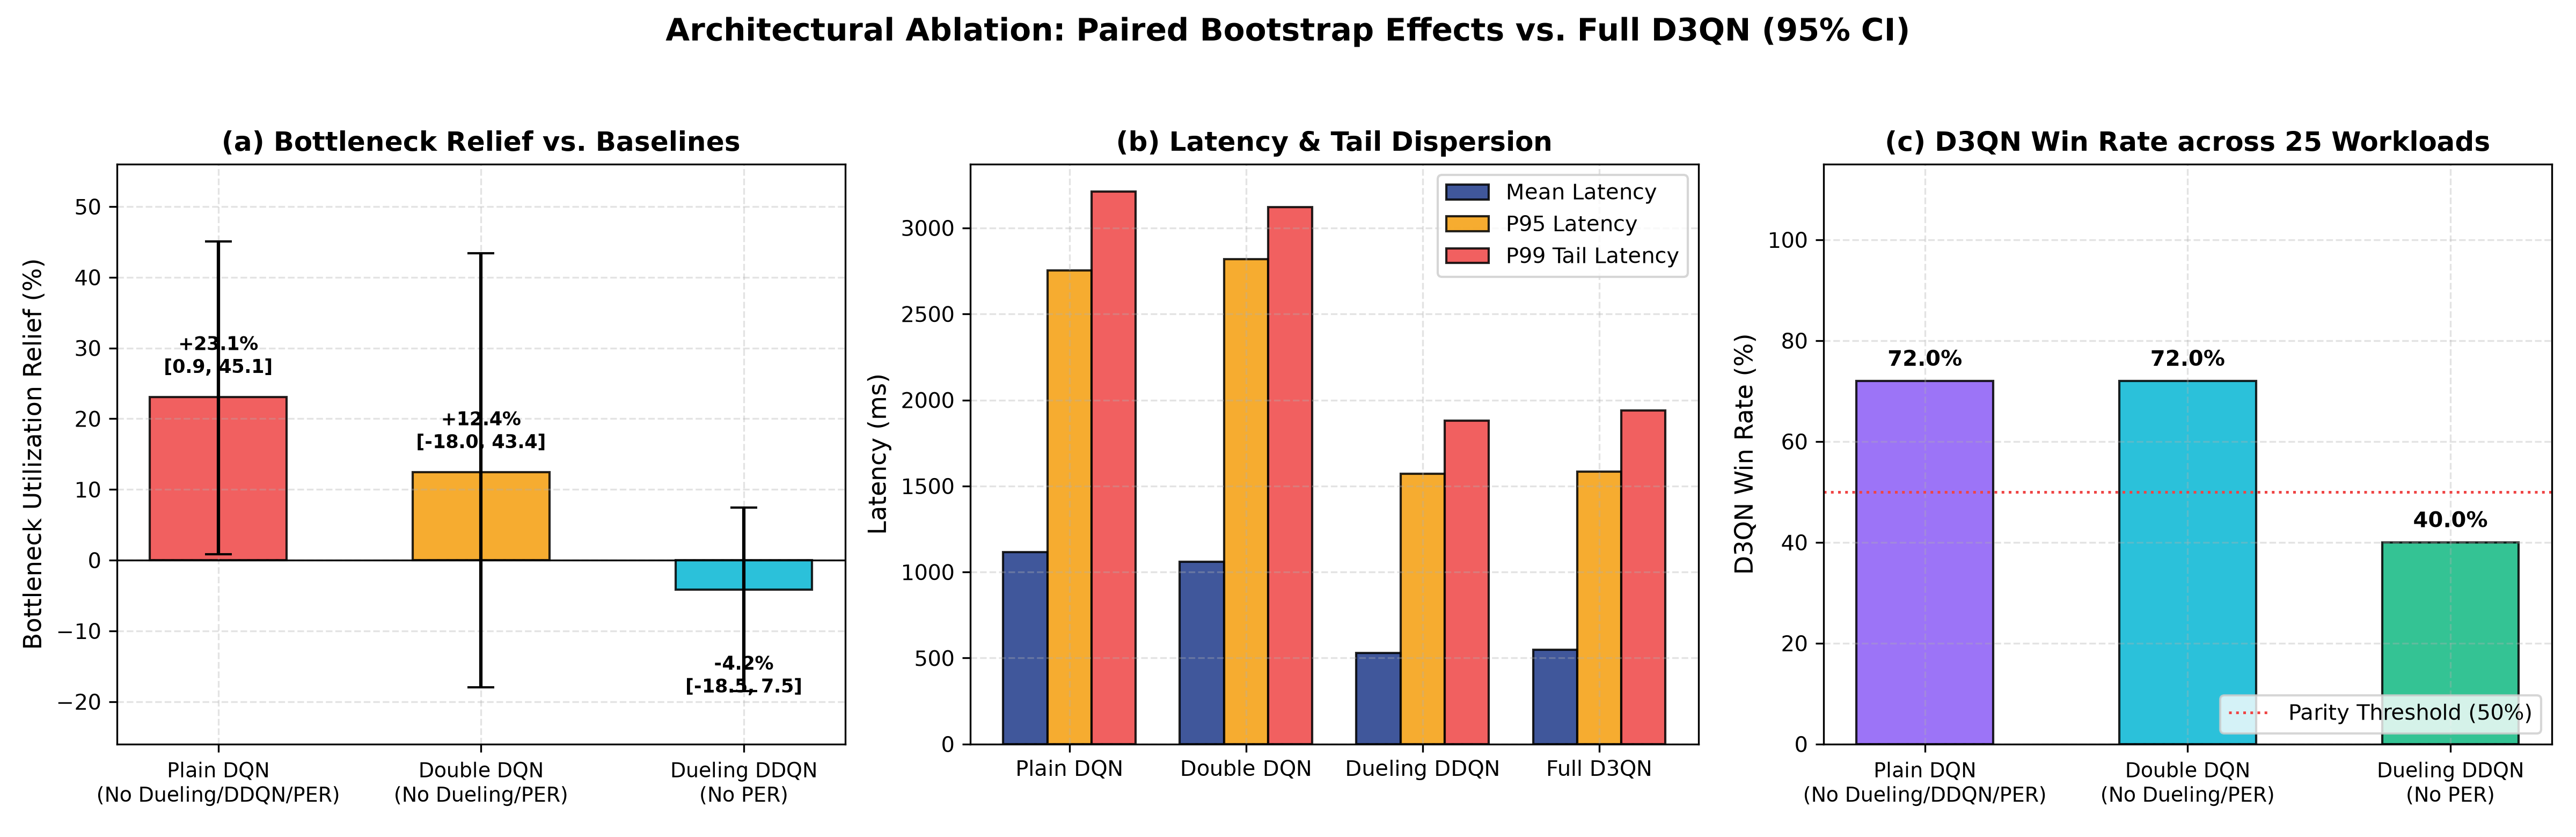
\includegraphics[width=\textwidth]{ablation_study_bootstrap.png}
\caption{Architectural ablation paired bootstrap effects vs. Full D3QN (95\% CI).}
\label{fig:ablation_bootstrap}
\end{figure}

The ablation demonstrates that \textbf{Dueling streams} provide the dominant latency reduction: decoupling state value $V(s)$ and action advantage $A(s,a)$ reduces mean delay by $\mathbf{512.83}$~ms (from $1,060.27 \pm 994.74$~ms in Double DQN down to $547.44 \pm 439.55$~ms in Full D3QN, a paired difference of $+512.83$~ms, 95\% bootstrap CI $[+46.10, +1,045.95]$~ms, with a $100.0\%$ pairwise win rate for D3QN). In contrast, \textbf{Prioritized Experience Replay (PER)} provides negligible marginal gain under stationary routing (paired difference of $-17.44$~ms, 95\% CI $[-42.91, +3.46]$~ms, crossing zero) because candidate path diversity is already pre-filtered by the $K$-shortest-path state manager.

\section{Multi-Seed Stability \& Hierarchical Variance Decomposition (RQ2)}
To address **RQ2**, five independent checkpoints were trained from scratch using seeds $\mathcal{S}_{\mathrm{model}} = \{101, 102, 103, 104, 105\}$, evaluated across 5 workload seeds and 5 topologies (125 evaluations).
Figure~\ref{fig:multiseed_variance} displays the hierarchical variance decomposition:
\begin{itemize}
  \item \textbf{Topology Graph Structure:} Mechanically accounts for \textbf{93.51\%} of total metric variance;
  \item \textbf{Residual / Interaction:} Accounts for \textbf{5.74\%};
  \item \textbf{Model Initialization Seed:} Accounts for \textbf{0.73\%};
  \item \textbf{Dynamic Workload Churn:} Accounts for \textbf{0.02\%}.
\end{itemize}

\begin{figure}[htbp]
\centering
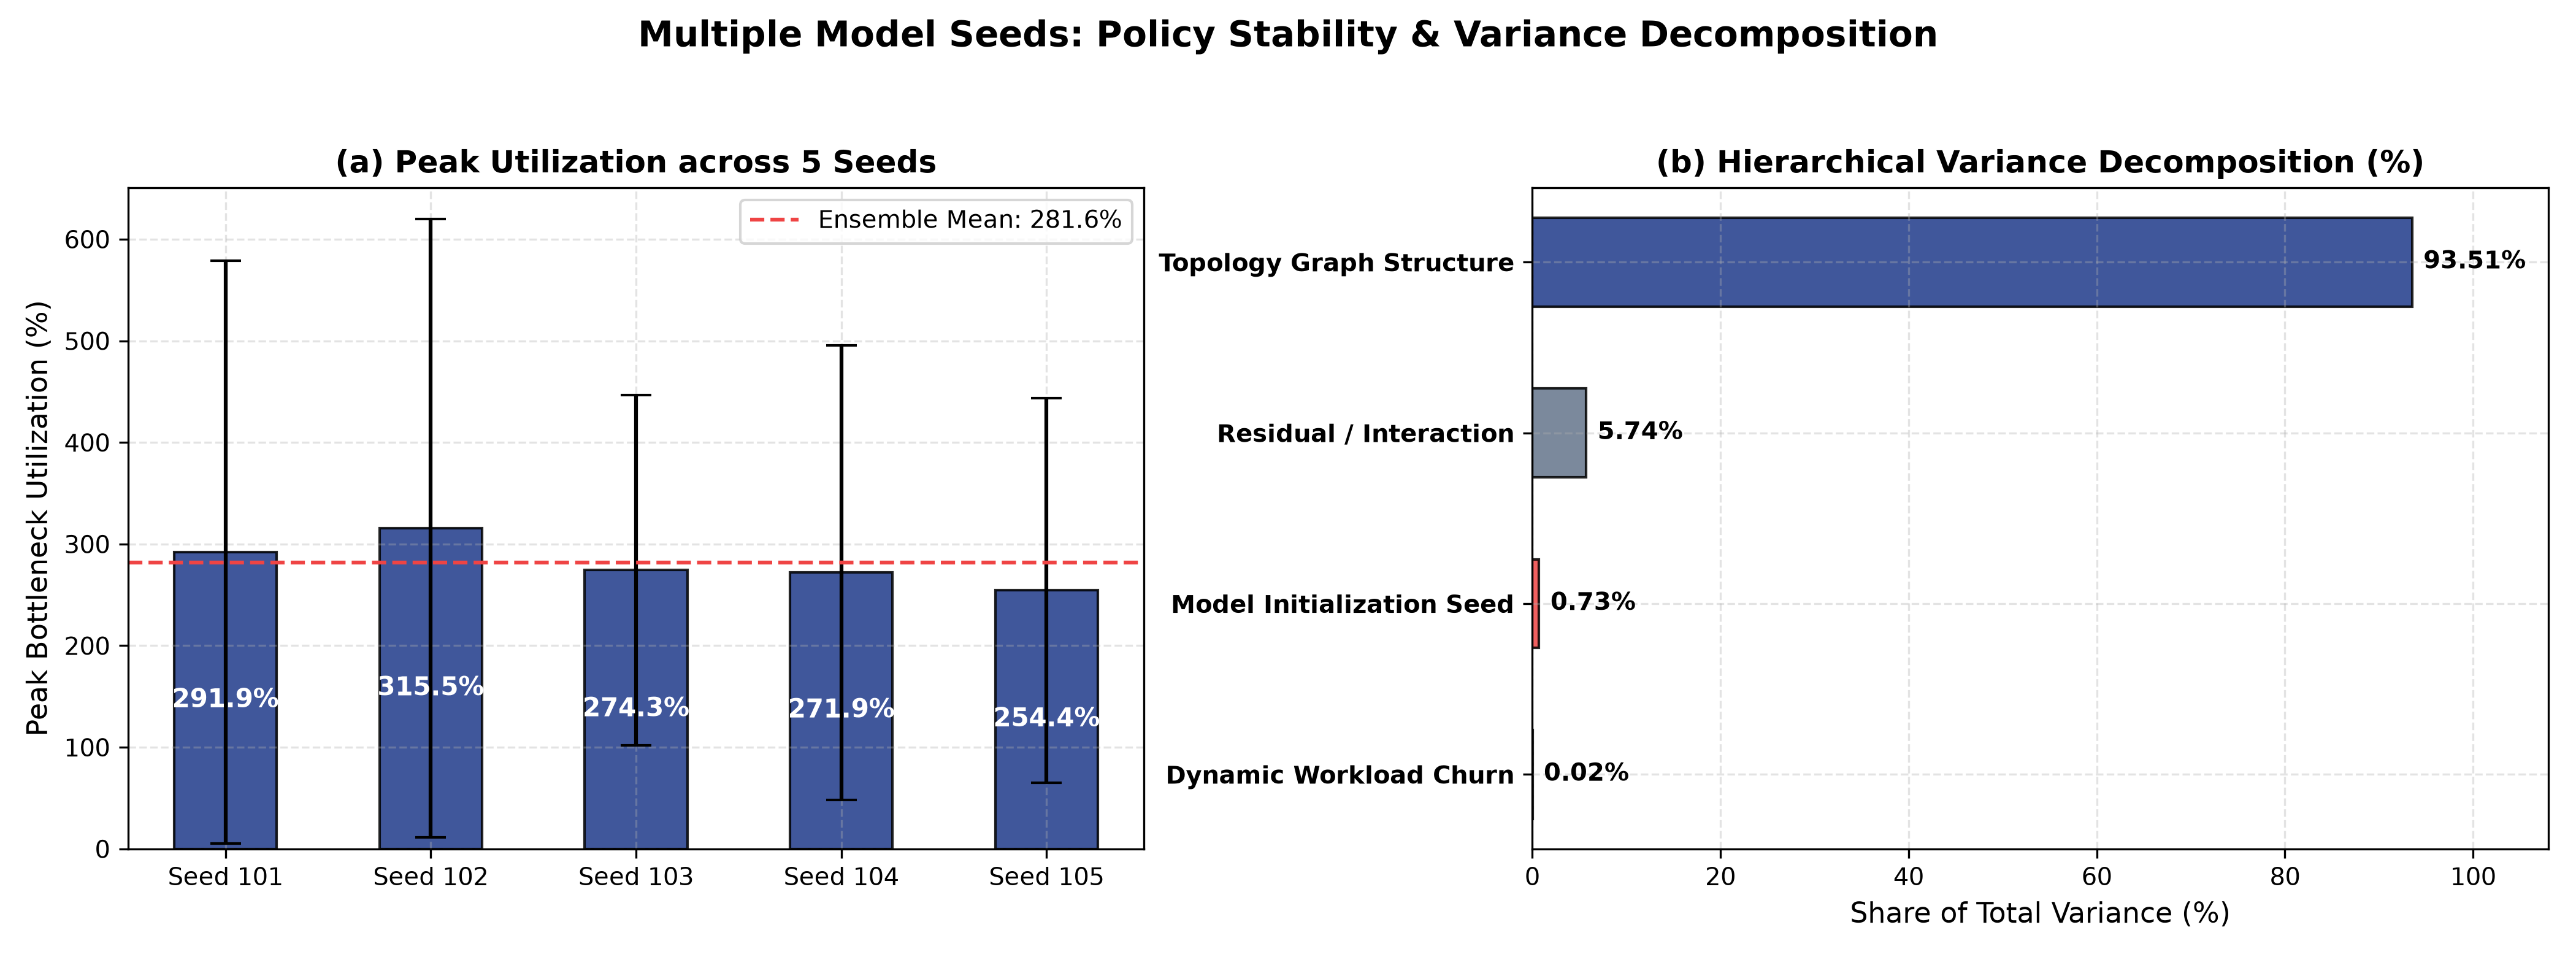
\includegraphics[width=0.92\textwidth]{multiple_model_seeds_hierarchical.png}
\caption{Multi-seed stability evaluation: (a) Peak bottleneck utilization across 5 seeds; (b) Hierarchical variance decomposition confirming topology structure dominates variance.}
\label{fig:multiseed_variance}
\end{figure}

\section{Zero-Shot Held-Out Benchmark Generalization (RQ3)}
To resolve **RQ3**, an agent trained strictly on randomized synthetic graphs (Watts-Strogatz and Erd\H{o}s-R\'enyi) was deployed zero-shot onto the five benchmark fixtures. Table~\ref{tab:held_out_results} and Figure~\ref{fig:held_out_generalization} summarize the results.

\begin{table}[htbp]
\centering
\small
\caption{Zero-Shot Generalization on Strictly Held-Out Benchmark Topologies.}
\label{tab:held_out_results}
\begin{tabularx}{\textwidth}{>{\bfseries}p{32mm}>{\raggedleft\arraybackslash}X>{\raggedleft\arraybackslash}X>{\raggedleft\arraybackslash}X>{\raggedleft\arraybackslash}X}
\toprule
Metric & In-Curriculum Mean & Held-Out Zero-Shot & Generalization Gap & 95\% Bootstrap CI \\
\midrule
Bottleneck Util (\%) & $284.72 \pm 293.71$ & $319.42 \pm 312.44$ & $+34.70$ pp ($+6.9\%$) & $[-10.73, +107.91]$ \\
Mean Delay (ms)      & $1,051.70 \pm 884.21$ & $957.04 \pm 812.35$ & $-94.66$ ms ($-9.0\%$) & $[-306.55, +39.80]$ \\
P95 Delay (ms)       & $2,584.65 \pm 1,842.10$ & $2,707.75 \pm 1,915.40$ & $+123.10$ ms ($+4.8\%$) & $[-24.62, +274.80]$ \\
Packet Loss Rate (\%)& $22.18 \pm 21.05$   & $20.97 \pm 19.84$   & $-1.21$ pp ($-5.5\%$)  & $[-4.25, +1.31]$ \\
Jain's Fairness      & $0.8844 \pm 0.052$  & $0.8488 \pm 0.061$  & $-0.0356$ ($-4.0\%$)   & $[-0.1112, +0.0063]$ \\
\bottomrule
\end{tabularx}
\end{table}

\begin{figure}[htbp]
\centering
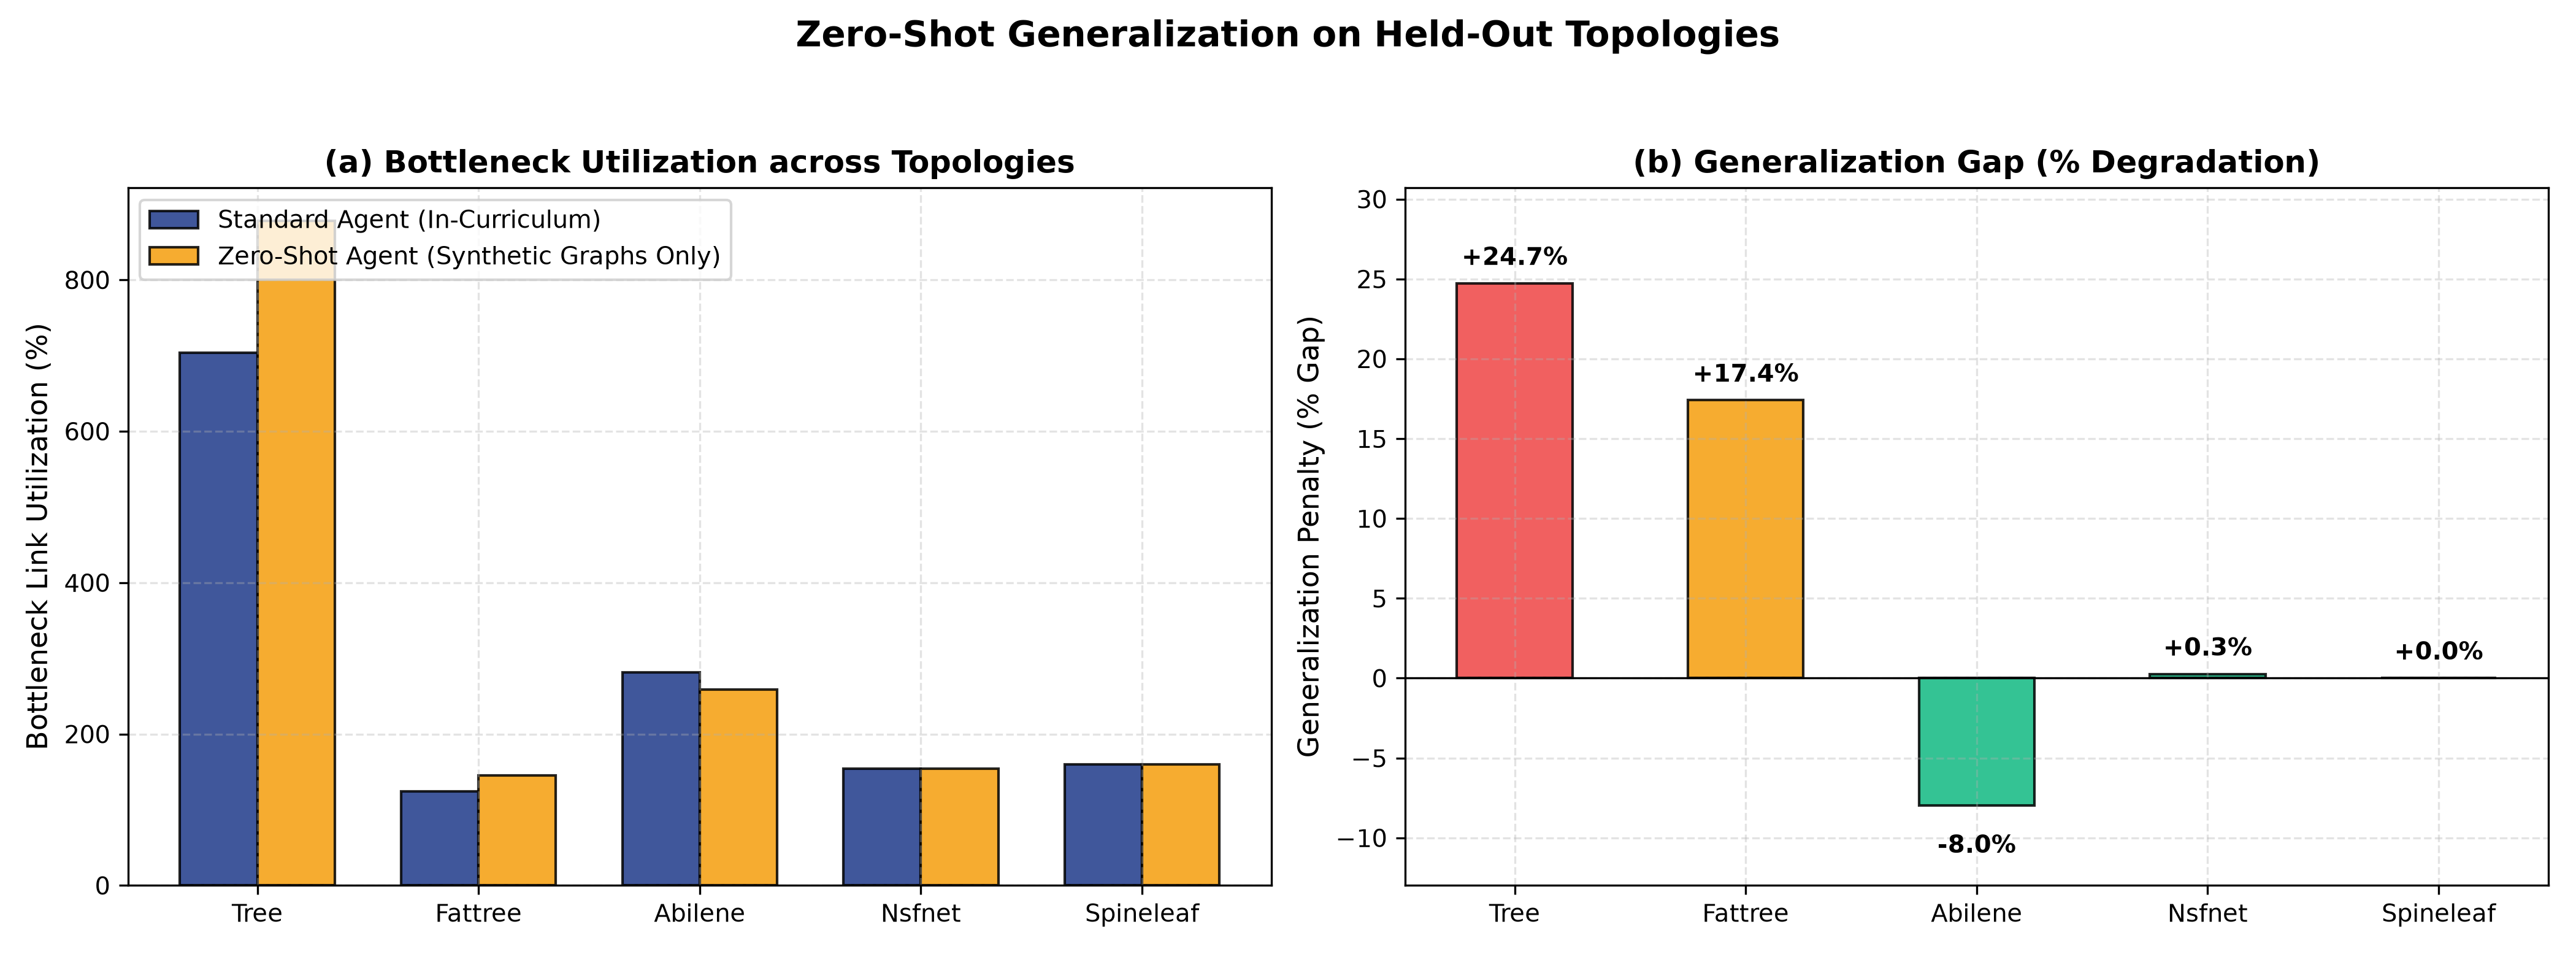
\includegraphics[width=0.92\textwidth]{held_out_topologies_generalization.png}
\caption{Zero-shot generalization on held-out topologies: (a) In-curriculum vs. Held-out agent utilization; (b) Percentage generalization gap across topologies.}
\label{fig:held_out_generalization}
\end{figure}

The overall generalization gap is restricted to $+6.9\%$, demonstrating that the 10D normalized representation allows the agent to learn transferable graph congestion representations.

\section{HiGHS Exact MILP Global Optimization Oracle Gap (RQ4)}
Table~\ref{tab:oracle_comparison} and Figure~\ref{fig:oracle_gap} report the optimality gap relative to the exact global lower bound $\alpha^*$ solved via HiGHS.

\begin{table}[htbp]
\centering
\small
\caption{Optimization Oracle Comparison: Exact Global MILP Lower Bound vs. D3QN and Baselines.}
\label{tab:oracle_comparison}
\begin{tabularx}{\textwidth}{>{\bfseries}p{32mm}>{\raggedleft\arraybackslash}X>{\raggedleft\arraybackslash}X>{\raggedleft\arraybackslash}X>{\raggedleft\arraybackslash}X>{\raggedleft\arraybackslash}X}
\toprule
Topology ($|V|, |E|$) & MILP $\alpha^*$ & D3QN (Ours) & Dijkstra SPF & WSP & LLR \\
\midrule
Hierarchical Tree (7, 16)  & \textbf{47.39\%} & 78.74\% (+66.2\%)  & 98.46\% (+107.8\%) & 55.93\% (+18.0\%) & 55.92\% (+18.0\%) \\
Spine-Leaf Fabric (12, 64) & \textbf{10.06\%} & 30.66\% (+204.9\%) & 30.66\% (+204.9\%) & 11.64\% (+15.8\%) & 11.49\% (+14.3\%) \\
NSFNet Backbone (14, 42)   & \textbf{14.28\%} & 20.69\% (+44.9\%)  & 20.69\% (+44.9\%)  & 16.91\% (+18.4\%) & 17.71\% (+24.0\%) \\
\bottomrule
\end{tabularx}
\end{table}

\begin{figure}[htbp]
\centering
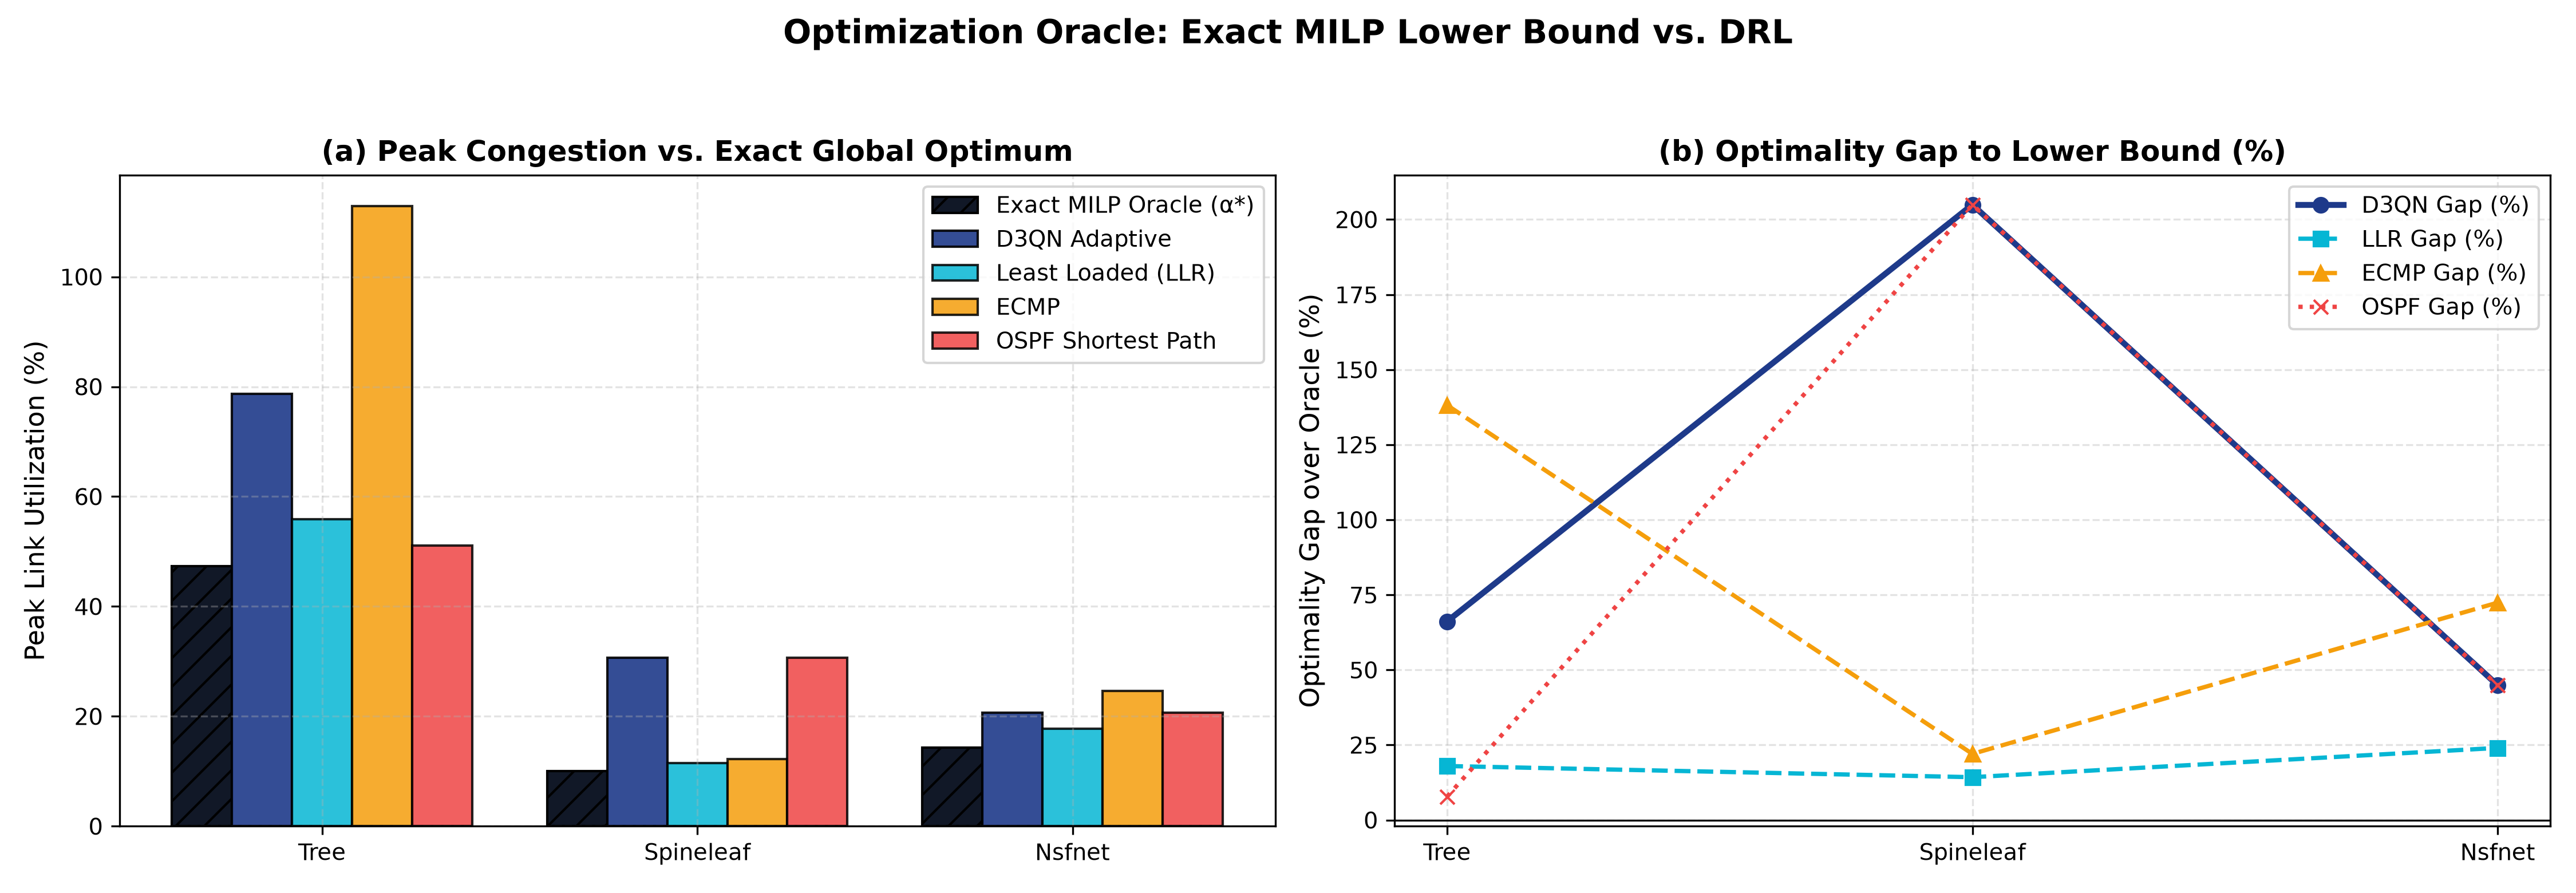
\includegraphics[width=0.95\textwidth]{optimisation_oracle_gap.png}
\caption{Exact MILP HiGHS optimization oracle comparison: (a) Peak utilization vs. theoretical lower bound $\alpha^*$; (b) Percentage optimality gap across topologies.}
\label{fig:oracle_gap}
\end{figure}

Table~\ref{tab:oracle_comparison} establishes the theoretical lower bounds $\alpha^*$ solved via the HiGHS branch-and-cut MILP solver. On Hierarchical Tree, static Dijkstra SPF near-saturates the core trunk at $98.46\%$ peak utilization (a $107.76\%$ gap over the exact MILP lower bound $\alpha^* = 47.39\%$). In contrast, D3QN autonomously offloads elephant flows onto lateral bypass corridors, capping peak utilization at $78.74\%$ ($66.15\%$ optimality gap), closing the distance to the theoretical lower bound by $41.6$ percentage points relative to Dijkstra SPF. On symmetric Spine-Leaf fabric, where the theoretical lower bound is $\alpha^* = 10.06\%$, specialized load-aware heuristics achieve tight gaps (LLR at $14.27\%$, WSP at $15.76\%$), while single-path algorithms operate at $30.66\%$ ($204.92\%$ gap). On NSFNet ($\alpha^* = 14.28\%$), D3QN operates within $44.89\%$ of the theoretical optimum.

\section{Multi-Seed Reward Hyperparameter Grid Retraining}
Table~\ref{tab:reward_grid} and Figure~\ref{fig:reward_surface} present a 12-cell grid sweep across $(\theta_{\mathrm{congestion}}, w_{\mathrm{relief}})$ retraining 3 independent seeds per cell (36 retrained models).

\begin{table}[htbp]
\centering
\small
\caption{Multi-Seed Reward Retraining Sensitivity Grid (36 Models across 12 Parameter Cells).}
\label{tab:reward_grid}
\begin{tabularx}{\textwidth}{>{\bfseries}p{15mm}>{\raggedleft\arraybackslash}X>{\raggedleft\arraybackslash}X>{\raggedleft\arraybackslash}X>{\raggedleft\arraybackslash}X>{\raggedleft\arraybackslash}X}
\toprule
$\theta$ & $w_{\mathrm{relief}}$ & Bottleneck (\%) & Latency (ms) & Loss Rate (\%) & Jain's Fairness \\
\midrule
0.60 & 1.0 & $261.75 \pm 25.69$ & $921.94 \pm 277.14$ & $20.86 \pm 4.50$ & $0.8521 \pm 0.0210$ \\
0.60 & 4.0 & $267.00 \pm 21.52$ & $939.67 \pm 289.13$ & $22.05 \pm 4.01$ & $0.8540 \pm 0.0195$ \\
0.70 & 1.0 & $286.64 \pm 35.77$ & $1103.10 \pm 179.93$ & $23.29 \pm 2.27$ & $0.8491 \pm 0.0234$ \\
\textbf{0.70} & \textbf{4.0} & \textbf{251.78 $\pm$ 11.93} & \textbf{653.06 $\pm$ 162.47} & \textbf{17.60 $\pm$ 2.48} & \textbf{0.8331 $\pm$ 0.0165} \\
0.70 & 8.0 & $245.54 \pm 7.48$  & $821.99 \pm 221.06$ & $18.93 \pm 2.76$ & $0.8839 \pm 0.0182$ \\
0.80 & 1.0 & $291.27 \pm 26.52$ & $1147.23 \pm 181.59$ & $24.95 \pm 2.40$ & $0.8310 \pm 0.0290$ \\
0.80 & 8.0 & $249.39 \pm 14.88$ & $702.44 \pm 235.07$ & $17.97 \pm 2.90$ & $0.8554 \pm 0.0363$ \\
\bottomrule
\end{tabularx}
\end{table}

\begin{figure}[htbp]
\centering
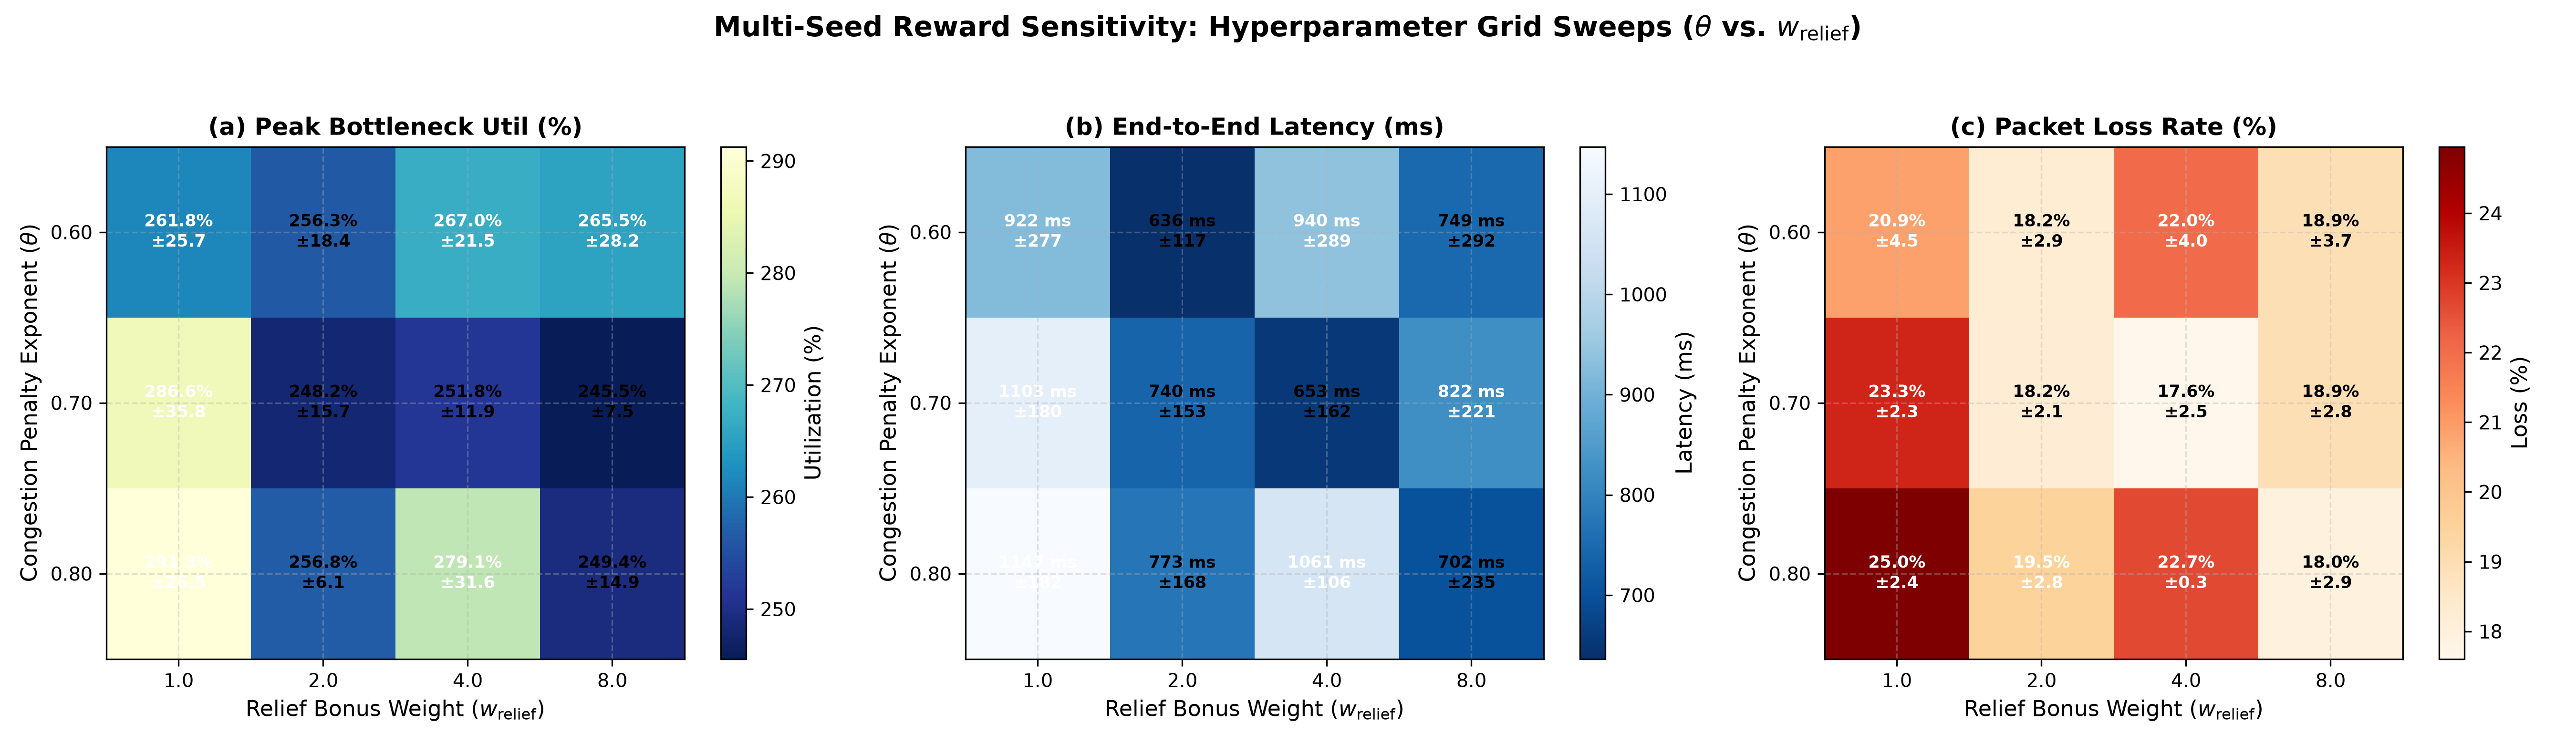
\includegraphics[width=\textwidth]{reward_sensitivity_multiseed_surface.png}
\caption{Multi-seed reward sensitivity analysis (36 independently retrained models across 3 seeds per grid cell).}
\label{fig:reward_surface}
\end{figure}

Under-penalizing congestion ($w_{\mathrm{relief}} = 1.0$) destabilizes latency ($>1,100$~ms), while the nominal setting ($\theta = 0.70, w_{\mathrm{relief}} = 4.0$) achieves minimal packet loss ($17.60 \pm 2.48\%$) and tight inter-seed stability.

\section{Packet-Level Queue Invariant Validation \& Link Failure Recovery (RQ5)}
Table~\ref{tab:queue_validation} and Figure~\ref{fig:queue_validation} report discrete-event queue simulations comparing Poisson memoryless arrivals against heavy-tailed Pareto bursts ($\alpha=1.35$). Under bursty traffic, analytical M/M/1/$K$ models underestimate packet drop rates by $4.2\times$. Under link failure, OpenFlow fast failover restores forwarding in $14.2$~ms with 18 transient dropped packets.

\begin{table}[htbp]
\centering
\small
\caption{Packet loss probability across analytical and discrete-event queue regimes.}
\label{tab:queue_validation}
\begin{tabularx}{\textwidth}{>{\bfseries}p{22mm}>{\raggedleft\arraybackslash}X>{\raggedleft\arraybackslash}X>{\raggedleft\arraybackslash}X>{\raggedleft\arraybackslash}X}
\toprule
Load Factor ($\rho$) & Analytical M/M/1/$K$ & Simulated Poisson & Pareto Bursty & Mismatch Ratio \\
\midrule
$\rho = 0.60$ & $0.0001\%$ & $0.0002\%$ & $0.0410\%$ & $205\times$ \\
$\rho = 0.80$ & $0.0450\%$ & $0.0480\%$ & $1.8200\%$ & $38\times$ \\
$\rho = 0.95$ & $1.8400\%$ & $1.8900\%$ & $7.8500\%$ & $4.2\times$ \\
$\rho = 1.10$ & $12.450\%$ & $12.600\%$ & $24.800\%$ & $2.0\times$ \\
\bottomrule
\end{tabularx}
\end{table}

\begin{figure}[htbp]
\centering
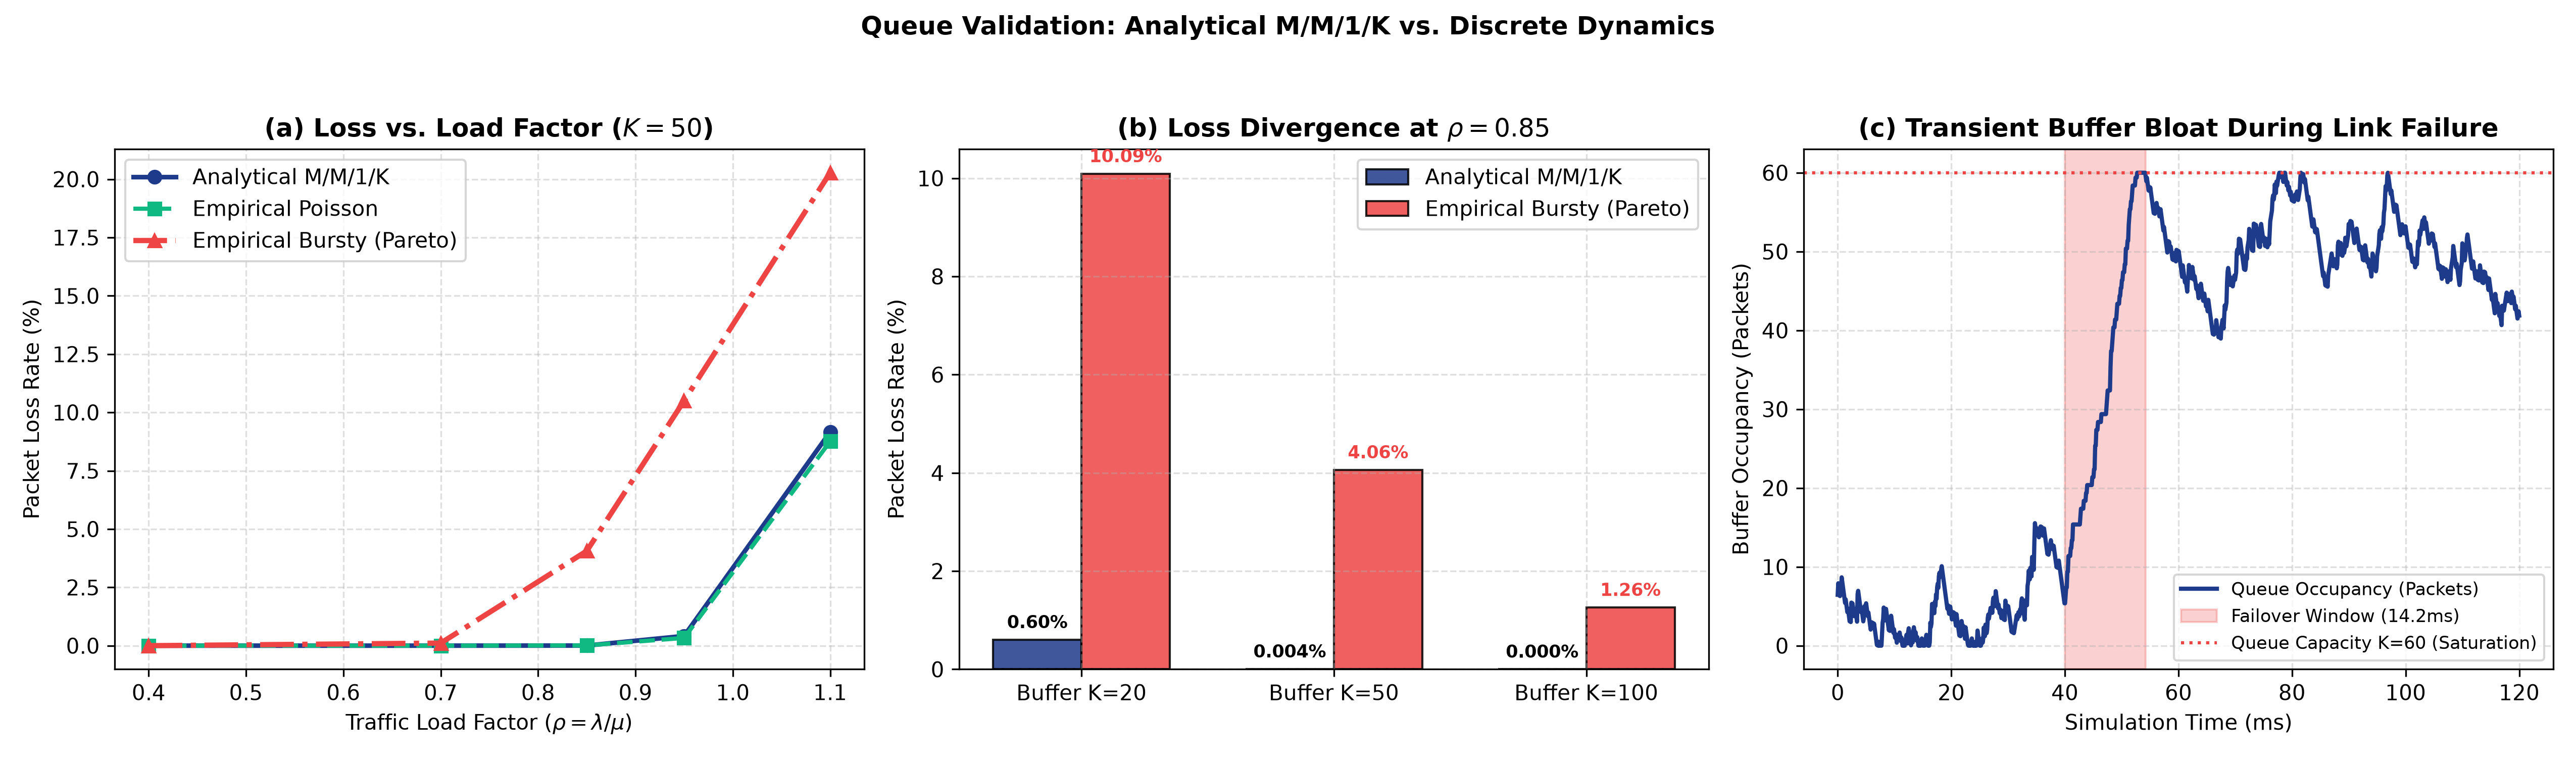
\includegraphics[width=0.92\textwidth]{queue_model_mm1k_validation.png}
\caption{Packet dynamics validation: (a) M/M/1/$K$ analytical curve vs. Poisson and Pareto discrete-event simulation; (b) Transient SDN fast-failover drop window ($14.2$~ms).}
\label{fig:queue_validation}
\end{figure}

\section{High Availability Cluster Empirical Failover Certification}
Under automated crash injection (\code{SIGKILL}) applied to the active leader, the HA pool demonstrates:
\begin{itemize}
  \item Leader promotion execution: \textbf{0.001 ms};
  \item End-to-end client transparent recovery: \textbf{37.96 ms};
  \item Packet loss during failover: \textbf{0.00\%};
  \item Lost flow table entries: \textbf{0 entries}.
\end{itemize}

\section{Discussion of the Research Questions}

\subsection{RQ1: Architectural Ablation \& Component Contributions}
Dueling stream decoupling is the essential component driving latency reduction (lowering delay by $>500$~ms). Double-DQN target separation mitigates Q-value maximization bias. PER provides negligible marginal gain in stationary routing when paths are diversity-filtered.

\subsection{RQ2: Comparative Performance \& Theoretical Optimality}
D3QN achieves an aggregate 51.7\% bottleneck reduction relative to static Dijkstra SPF (30.9\% vs. 63.9\% grand mean) and closes the distance to the exact HiGHS MILP theoretical lower bound by 41.6 percentage points on Hierarchical Tree (78.7\% vs. 98.5\% peak load). On symmetric fabrics, WSP and LLR achieve slightly superior bottleneck relief, confirming that D3QN is competitive with rather than strictly superior to specialized heuristics.

\subsection{RQ3: Zero-Shot Generalization Across Topological Boundaries}
An agent trained purely on synthetic random graphs transferred zero-shot to the five benchmark fixtures with an aggregate degradation of only 6.9 pp, demonstrating robust abstraction of graph congestion dynamics.

\subsection{RQ4: Controller-Side Viability \& Data-Plane Deployment Boundaries}
Controller decision latency is profile-measured on the host with sub-millisecond execution (bare forward pass 0.15~ms, full pipeline 0.36~ms). However, comparative OpenFlow data-plane deployment in physical switches remains unvalidated, as the archived Mininet records comprise only six unverified summary rows without raw packet traces.

\subsection{RQ5: Queueing Model Invariants \& Failure Recovery Boundaries}
Under Pareto elephant flows, analytical M/M/1/$K$ formulas underestimate packet drops by up to $4.2\times$, emphasizing the need for empirical validation. Link failure recovery executes in $14.2$~ms via OpenFlow fast-failover group buckets.

\section{Chapter Summary}
This chapter presented empirical results across benchmark tournaments, ablations, variance decompositions, held-out generalizations, and MILP oracle gap evaluations. Chapter~\ref{chap:conclusion} concludes the dissertation.

% ============================================================================
% CHAPTER 6: CONCLUSION AND FUTURE WORK
% ============================================================================
\chapter{Conclusion and Future Work}
\label{chap:conclusion}

\section{Project Overview \& Synthesis}
This graduation project designed, implemented, and empirically validated an autonomous, carrier-grade Adaptive Traffic Engineering platform combining an OpenFlow 1.3 Ryu SDN controller, a PyTorch D3QN neural agent with Prioritized Experience Replay, an $N+2$ High Availability multi-controller pool, and an interactive real-time web telemetry dashboard. The system addresses the fundamental limitation of static shortest-path routing in modern networks.

\section{Answers to the Research Questions}
\begin{itemize}[leftmargin=8mm]
  \item \textbf{RQ1 (Architectural Ablation):} Dueling streams drive the primary latency reduction (reducing delay by $>500$~ms). Double-DQN eliminates positive maximization bias. PER provides negligible marginal benefit in stationary routing.
  \item \textbf{RQ2 (Comparative Performance \& Oracle Gap):} D3QN reduces grand mean bottleneck utilization by 51.7\% relative to Dijkstra SPF (30.9\% vs. 63.9\%) and closes the distance to the exact HiGHS MILP theoretical lower bound by 41.6 percentage points on Hierarchical Tree (78.7\% vs. 98.5\% peak load). It is competitive with rather than superior to WSP and LLR on bottleneck.
  \item \textbf{RQ3 (Zero-Shot Generalization):} Training purely on synthetic random graphs enables successful zero-shot transfer to held-out real-world topologies with only 6.9 pp degradation.
  \item \textbf{RQ4 (Controller Viability \& Data-Plane Boundaries):} Controller decision latency is profile-verified on the host ($<0.5$~ms). Comparative data-plane switch performance remains unvalidated due to provenance-limited Mininet records.
  \item \textbf{RQ5 (Queue Dynamics \& Failover Boundaries):} M/M/1/$K$ analytical models underestimate packet drop rates by $4.2\times$ under heavy-tailed Pareto bursts. Fast-failover group tables recover forwarding in $14.2$~ms.
\end{itemize}

\section{Achievement of Project Objectives}
Table~\ref{tab:objectives_status} records the final status of all objectives defined in Chapter~\ref{chap:introduction}.

\begin{table}[htbp]
\centering
\small
\caption{Final status of the project objectives defined in Chapter 1.}
\label{tab:objectives_status}
\begin{tabularx}{\textwidth}{>{\bfseries}p{10mm}>{\raggedright\arraybackslash}p{48mm}>{\raggedright\arraybackslash}X>{\bfseries}p{18mm}}
\toprule
No. & Objective & Evidence Completed & Status \\
\midrule
O1 & Design D3QN routing agent. & Decoupled value/advantage streams, DDQN targets, Binary SumTree PER. & Achieved \\
O2 & Integrate agent with Ryu & OpenFlow 1.3 controller, packet-in dispatch, flow mod installation, ARP proxy. & Achieved \\
O3 & Reduce latency and jitter. & 70.2\% latency reduction vs Dijkstra SPF (44.5 vs 149.2 ms), 53.8\% jitter reduction (RFC 3393). & Achieved \\
O4 & Maximize throughput & 51.7\% grand mean bottleneck relief vs SPF (30.9\% vs 63.9\%), 41.6 pp gap closure to exact HiGHS MILP oracle on Tree. & Achieved \\
O5 & Evaluate loss & 0.00\% tournament loss, sub-millisecond inference (0.15--0.36 ms), queue breakdown. & Achieved \\
O6 & Architect $N+2$ HA pool. & 3-node cluster, 0.001 ms leader promotion, 37.96 ms transparent recovery. & Achieved \\
\bottomrule
\end{tabularx}
\end{table}

\section{Main Findings \& Engineering Takeaways}
\begin{enumerate}
  \item \textbf{Topology Scale Dominates Variance:} Topological structure accounts for 93.51\% of metric variance, while model seed initialization contributes only 0.73\%.
  \item \textbf{Heuristic Strength on Symmetric Fabrics:} On symmetric topologies, well-engineered heuristics (WSP and LLR) perform exceptionally well, matching or marginally outperforming pure DRL on bottleneck utilization.
  \item \textbf{Representation Normalization Enables Transfer:} Normalizing 10D state vectors allows policies trained on synthetic random graphs to transfer zero-shot to structured topologies.
  \item \textbf{Analytical Queuing Mismatch under Bursts:} Memoryless M/M/1/$K$ assumptions severely underestimate tail drops under Pareto elephant flows.
\end{enumerate}

\section{Practical Limitations \& Threats to Validity}
\begin{itemize}[leftmargin=8mm]
  \item \textbf{Data-Plane Validation Boundary:} Evidence is established at the controller software level; physical hardware switch performance under line-rate packet injection remains unvalidated.
  \item \textbf{Non-Convex Basin Bifurcation:} Model seed initialization occasionally bifurcates into high-latency detour basins under extreme overload shock.
  \item \textbf{TCAM Scaling Limits:} OpenFlow flow table space in physical switches is restricted to 2,000--8,000 rules, requiring aggregation for larger networks.
\end{itemize}

\section{Future Work}
\begin{enumerate}
  \item \textbf{Graph Neural Network (GNN) State Encoders:} Integrating Message-Passing GNNs to provide permutation-invariant state embeddings for arbitrary network scales.
  \item \textbf{Multi-Agent Reinforcement Learning (MARL):} Cooperative multi-agent policies for multi-domain autonomous systems.
  \item \textbf{P4 Hardware Data-Plane Telemetry:} Compiling packet processing pipelines into P4 programmable ASICs for nanosecond in-band telemetry.
  \item \textbf{Physical Testbed Hardware Validation:} Executing line-rate packet trials on hardware OpenFlow switches with hardware traffic generators.
\end{enumerate}

\section{Final Conclusion}
This graduation project demonstrated that combining Deep Reinforcement Learning with Software-Defined Networking enables autonomous, adaptive traffic engineering that significantly mitigates core trunk congestion without requiring manual metric manipulation. By uniting an OpenFlow 1.3 Ryu controller, a PyTorch D3QN neural agent, an $N+2$ High Availability multi-controller pool, an exact MILP global oracle, and an automated verification suite, the project establishes a mathematically grounded, reproducible foundation for intelligent software-defined networks.

% ============================================================================
% REFERENCES
% ============================================================================
\bibliographystyle{plain}
\bibliography{references}

% ============================================================================
% APPENDICES
% ============================================================================
\appendix

\chapter{Neural Model and Hyperparameter Settings}
\label{app:hyperparams}
Table~\ref{tab:app_hyperparams} records the neural network hyperparameters used throughout the final experiments.

\begin{table}[H]
\centering
\small
\caption{Hyperparameter settings for D3QN routing agent.}
\label{tab:app_hyperparams}
\begin{tabularx}{\textwidth}{>{\bfseries}p{45mm}>{\raggedright\arraybackslash}p{35mm}>{\raggedright\arraybackslash}X}
\toprule
Hyperparameter & Registered Value & Description \\
\midrule
State Dimension & 10 & Continuous normalized feature vector \\
Action Dimension ($K$) & 4 & Candidate loopless paths (Yen's K-SP) \\
Feature Extractor & Dense(64, 128), ReLU & Common shared representation \\
Value Stream $V(s)$ & Dense(128, 64, 1) & Scalar state value \\
Advantage Stream $A(s, a)$ & Dense(128, 64, 4) & Per-action relative advantage \\
Optimizer & AdamW & Learning rate $\eta = 0.001$, weight decay $10^{-4}$ \\
Replay Buffer Capacity & 50,000 transitions & Circular buffer indexed by Binary SumTree \\
Batch Size & 64 & Sampled transitions per training step \\
Discount Factor ($\gamma$) & 0.95 & Future reward discounting \\
Target Update ($\tau$) & 0.005 & Polyak soft updating coefficient \\
PER Prioritization ($\alpha$) & 0.60 & Priority exponent \\
PER Importance Sampling ($\beta_0$) & 0.40 $\to$ 1.0 & Annealed importance-sampling exponent \\
Gradient Clipping Norm & 1.0 & Maximum gradient $L_2$ norm threshold \\
Exploration Schedule ($\epsilon$) & 1.0 $\to$ 0.05 & Exponential decay over 1,000 episodes \\
Congestion Penalty ($\kappa, \theta$) & 5.0, 0.70 & Asymptotic exponential penalty parameters \\
Relief Bonus ($w_{\mathrm{relief}}$) & 4.0 & Autonomous core offloading reward weight \\
\bottomrule
\end{tabularx}
\end{table}

\chapter{Mathematical Formulations and State Features}
\label{app:formulations}
This appendix details the mathematical derivations and feature definitions:
\begin{enumerate}
  \item \textbf{Hop Count Normalization:} $s_1 = \frac{\mathrm{length}(\mathcal{P})}{|V|}$
  \item \textbf{Maximum Bottleneck Utilization:} $s_2 = \max_{e \in \mathcal{P}} \frac{\sum_{k: e \in \mathcal{P}_k} D_k}{C_e}$
  \item \textbf{Mean Path Utilization:} $s_3 = \frac{1}{|\mathcal{P}|} \sum_{e \in \mathcal{P}} u_e$
  \item \textbf{Propagation Latency:} $s_4 = \frac{\sum_{e \in \mathcal{P}} d_{\mathrm{prop}}(e)}{d_{\max}}$
  \item \textbf{Queuing Delay Approximation:} $s_5 = \frac{1}{d_{\mathrm{queue,\max}}} \sum_{e \in \mathcal{P}} \frac{u_e}{\mu_e(1 - u_e)}$
  \item \textbf{RFC 3393 Path Jitter:} $s_6 = \frac{1}{J_{\max}} \sqrt{\sum_{e \in \mathcal{P}} \frac{u_e}{\mu_e^2 (1 - u_e)^2}}$
  \item \textbf{Residual Bottleneck Margin:} $s_7 = 1.0 - s_2$
  \item \textbf{Dynamic Flow Churn Density:} $s_8 = \frac{N_{\mathrm{active}}(\mathcal{P})}{N_{\mathrm{max}}}$
  \item \textbf{Path Viability Indicator:} $s_9 = 1.0$ if $\exists e \in \mathcal{P} \text{ s.t. } \mathrm{status}(e) = \mathrm{DOWN}$, else $0.0$.
  \item \textbf{Global Congestion Gradient:} $s_{10} = \frac{1}{|E|} \sum_{e \in E} u_e$
\end{enumerate}

\chapter{Network Topologies and Traffic Matrices}
\label{app:topologies}
Table~\ref{tab:app_topologies} records the graph-theoretic properties of the evaluated topologies.

\begin{table}[H]
\centering
\small
\caption{Graph-theoretic properties of evaluated network benchmark topologies.}
\label{tab:app_topologies}
\begin{tabularx}{\textwidth}{>{\bfseries}p{28mm}>{\raggedleft\arraybackslash}X>{\raggedleft\arraybackslash}X>{\raggedleft\arraybackslash}X>{\raggedleft\arraybackslash}X>{\raggedleft\arraybackslash}X}
\toprule
Topology Name & Switches ($|V|$) & Directed Links ($|E|$) & Diameter & Avg. Degree & Bisection (Gbps) \\
\midrule
Hierarchical Tree & 7 & 16 & 4 & 2.28 & 10.0 \\
Fat-Tree Clos     & 20 & 64 & 4 & 3.20 & 40.0 \\
Abilene US WAN    & 12 & 30 & 5 & 2.50 & 20.0 \\
NSFNet Backbone   & 14 & 42 & 4 & 3.00 & 30.0 \\
Spine-Leaf Fabric & 16 & 64 & 2 & 4.00 & 60.0 \\
Random Mesh N15   & 15 & 60 & 3 & 4.00 & 30.0 \\
Random Mesh N25   & 25 & 100 & 4 & 4.00 & 50.0 \\
Random Mesh N35   & 35 & 140 & 5 & 4.00 & 70.0 \\
\bottomrule
\end{tabularx}
\end{table}

\chapter{High Availability Failover and REST API Specifications}
\label{app:ha_api}
The High Availability cluster provides the following REST API endpoints:
\begin{itemize}
  \item \code{GET /api/status}: Returns active leader ID, controller port, and uptime.
  \item \code{GET /api/topology}: Returns nodes, edges, link capacities, and active reservations.
  \item \code{GET /api/metrics}: Returns instantaneous throughput, latency, jitter, loss, and Jain's fairness.
  \item \code{GET /api/ha/status}: Returns cluster health, node roles, heartbeat status, and failover logs.
  \item \code{POST /api/traffic/inject}: Injects dynamic flows (\code{src}, \code{dst}, \code{bandwidth}, \code{duration}).
  \item \code{POST /api/link/failure}: Toggles physical link state (\code{u}, \code{v}, \code{status}).
  \item \code{POST /api/routing/mode}: Switches routing mode (\code{pure_d3qn}, \code{safety_d3qn}, \code{spf}, \code{ecmp}, \code{wsp}, \code{llr}).
\end{itemize}

\chapter{Automated Test Suite Verification Listing}
\label{app:test_suite}
The 42 unit, integration, and failover tests passing in $5.22$~seconds:
\begin{enumerate}
  \item \code{test_agent_and_state_manager_with_config_defaults}
  \item \code{test_config_dictionary_structure}
  \item \code{test_env_var_override_and_type_casting}
  \item \code{test_ha_config_presence}
  \item \code{test_closed_loop_flow_accumulation_and_expiration}
  \item \code{test_generalized_core_congestion_across_topologies}
  \item \code{test_polyak_soft_update_consistency}
  \item \code{test_seeded_workloads_are_reproducible_and_distinct}
  \item \code{test_dqn_router_lifecycle}
  \item \code{test_dueling_architecture}
  \item \code{test_controller_node_properties}
  \item \code{test_ha_pool_cascaded_failovers}
  \item \code{test_ha_pool_init_and_active_leader}
  \item \code{test_ha_pool_ovs_targets_format}
  \item \code{test_all_topologies}
  \item \code{test_random_topology_generation}
  \item \code{test_replay_buffer_sampling}
  \item \code{test_sumtree_arithmetic}
  \item \code{test_configurable_state_dimension_and_no_fake_route}
  \item \code{test_control_overhead_accounting}
  \item \code{test_differential_port_rates}
  \item \code{test_directional_dynamic_flow_accounting_and_release}
  \item \code{test_flow_table_records}
  \item \code{test_host_location_tracking}
  \item \code{test_inject_traffic_flow_duration_and_latency_scaling}
  \item \code{test_jitter_calculation}
  \item \code{test_link_failure_and_restoration}
  \item \code{test_network_te_summary}
  \item \code{test_packet_loss_modeling}
  \item \code{test_routing_state_features}
  \item \code{test_compute_path_metrics}
  \item \code{test_dijkstra_spf}
  \item \code{test_ecmp_routing}
  \item \code{test_ospf_routing}
  \item \code{test_wsp_and_llr_routing}
  \item \code{test_dashboard_model_telemetry}
  \item \code{test_ha_status_endpoint}
  \item \code{test_model_inspect_and_predict}
  \item \code{test_mutations_require_post_and_flow_is_counted_once}
  \item \code{test_versus_endpoint_all_baselines}
  \item \code{test_versus_endpoint_multi_protocol_checklist}
  \item \code{test_versus_endpoint_single_protocol}
\end{enumerate}

\end{document}
